\documentclass[ALICE,manyauthors]{ALICE_analysis_notes}

\usepackage{array}
\usepackage{enumitem}
\usepackage[hidelinks,linktocpage=true,hyperfigures=false,hyperfootnotes=false]{hyperref}
\usepackage{lineno}
\usepackage{multirow}
\usepackage{perpage}
\usepackage{rotating}
\usepackage{xcolor}
\usepackage{appendix}

\PHnumber{ALICE-ANA-2022-xxx} 
\PHdate{\today}
\MakePerPage{footnote}
\renewcommand{\thefootnote}{\alph{footnote}}
% 1) SYSTEMS 
\newcommand{\pp}           {pp\xspace}
\newcommand{\ppbar}        {\mbox{$\mathrm {p\overline{p}}$}\xspace}
\newcommand{\XeXe}         {\mbox{Xe--Xe}\xspace}
\newcommand{\PbPb}         {\mbox{Pb--Pb}\xspace}
\newcommand{\pA}           {\mbox{pA}\xspace}
\newcommand{\pPb}          {\mbox{p--Pb}\xspace}
\newcommand{\AuAu}         {\mbox{Au--Au}\xspace}
\newcommand{\dAu}          {\mbox{d--Au}\xspace}

% 2) QUANTITIES 
\newcommand{\s}            {\ensuremath{\sqrt{s}}\xspace}
\newcommand{\snn}          {\ensuremath{\sqrt{s_{\mathrm{NN}}}}\xspace}
\newcommand{\pt}           {\ensuremath{p_{\rm T}}\xspace}
\newcommand{\meanpt}       {$\langle p_{\mathrm{T}}\rangle$\xspace}
\newcommand{\ycms}         {\ensuremath{y_{\rm CMS}}\xspace}
\newcommand{\ylab}         {\ensuremath{y_{\rm lab}}\xspace}
\newcommand{\etarange}[1]  {\mbox{$\left | \eta \right |~<~#1$}}
\newcommand{\yrange}[1]    {\mbox{$\left | y \right |~<~#1$}}
\newcommand{\dndy}         {\ensuremath{\mathrm{d}N_\mathrm{ch}/\mathrm{d}y}\xspace}
\newcommand{\dndeta}       {\ensuremath{\mathrm{d}N_\mathrm{ch}/\mathrm{d}\eta}\xspace}
\newcommand{\avdndeta}     {\ensuremath{\langle\dndeta\rangle}\xspace}
\newcommand{\dNdy}         {\ensuremath{\mathrm{d}N_\mathrm{ch}/\mathrm{d}y}\xspace}
\newcommand{\Npart}        {\ensuremath{N_\mathrm{part}}\xspace}
\newcommand{\Ncoll}        {\ensuremath{N_\mathrm{coll}}\xspace}
\newcommand{\dEdx}         {\ensuremath{\textrm{d}E/\textrm{d}x}\xspace}
\newcommand{\RpPb}         {\ensuremath{R_{\rm pPb}}\xspace}

% 3) ENERGIES, UNITS
\newcommand{\nineH}        {$\sqrt{s}~=~0.9$~Te\kern-.1emV\xspace}
\newcommand{\seven}        {$\sqrt{s}~=~7$~Te\kern-.1emV\xspace}
\newcommand{\twoH}         {$\sqrt{s}~=~0.2$~Te\kern-.1emV\xspace}
\newcommand{\twosevensix}  {$\sqrt{s}~=~2.76$~Te\kern-.1emV\xspace}
\newcommand{\five}         {$\sqrt{s}~=~5.02$~Te\kern-.1emV\xspace}
\newcommand{\thirteen}     {$\sqrt{s}~=~13$~Te\kern-.1emV\xspace} %kimc
\newcommand{\twosevensixnn}{$\sqrt{s_{\mathrm{NN}}}~=~2.76$~Te\kern-.1emV\xspace}
\newcommand{\fivenn}       {$\sqrt{s_{\mathrm{NN}}}~=~5.02$~Te\kern-.1emV\xspace}
\newcommand{\LT}           {L{\'e}vy-Tsallis\xspace}
\newcommand{\GeVc}         {Ge\kern-.1emV/$c$\xspace}
\newcommand{\MeVc}         {Me\kern-.1emV/$c$\xspace}
\newcommand{\TeV}          {Te\kern-.1emV\xspace}
\newcommand{\GeV}          {Ge\kern-.1emV\xspace}
\newcommand{\MeV}          {Me\kern-.1emV\xspace}
\newcommand{\GeVmass}      {Ge\kern-.2emV/$c^2$\xspace}
\newcommand{\MeVmass}      {Me\kern-.2emV/$c^2$\xspace}
\newcommand{\lumi}         {\ensuremath{\mathcal{L}}\xspace}

% 4) DETECTORS 
\newcommand{\ITS}          {\rm{ITS}\xspace}
\newcommand{\TOF}          {\rm{TOF}\xspace}
\newcommand{\ZDC}          {\rm{ZDC}\xspace}
\newcommand{\ZDCs}         {\rm{ZDCs}\xspace}
\newcommand{\ZNA}          {\rm{ZNA}\xspace}
\newcommand{\ZNC}          {\rm{ZNC}\xspace}
\newcommand{\SPD}          {\rm{SPD}\xspace}
\newcommand{\SDD}          {\rm{SDD}\xspace}
\newcommand{\SSD}          {\rm{SSD}\xspace}
\newcommand{\TPC}          {\rm{TPC}\xspace}
\newcommand{\TRD}          {\rm{TRD}\xspace}
\newcommand{\VZERO}        {\rm{V0}\xspace}
\newcommand{\VZEROA}       {\rm{V0A}\xspace}
\newcommand{\VZEROC}       {\rm{V0C}\xspace}
\newcommand{\Vdecay} 	   {\ensuremath{V^{0}}\xspace}

% 4) PARTICLE SPECIES 
\newcommand{\ee}           {\ensuremath{e^{+}e^{-}}} 
\newcommand{\pip}          {\ensuremath{\pi^{+}}\xspace}
\newcommand{\pim}          {\ensuremath{\pi^{-}}\xspace}
\newcommand{\kap}          {\ensuremath{\rm{K}^{+}}\xspace}
\newcommand{\kam}          {\ensuremath{\rm{K}^{-}}\xspace}
\newcommand{\pbar}         {\ensuremath{\rm\overline{p}}\xspace}
\newcommand{\kzero}        {\ensuremath{{\rm K}^{0}_{\rm{S}}}\xspace}
\newcommand{\lmb}          {\ensuremath{\Lambda}\xspace}
\newcommand{\almb}         {\ensuremath{\overline{\Lambda}}\xspace}
\newcommand{\Om}           {\ensuremath{\Omega^-}\xspace}
\newcommand{\Mo}           {\ensuremath{\overline{\Omega}^+}\xspace}
\newcommand{\X}            {\ensuremath{\Xi^-}\xspace}
\newcommand{\Ix}           {\ensuremath{\overline{\Xi}^+}\xspace}
\newcommand{\Xis}          {\ensuremath{\Xi^{\pm}}\xspace}
\newcommand{\Oms}          {\ensuremath{\Omega^{\pm}}\xspace}
\newcommand{\degree}       {\ensuremath{^{\rm o}}\xspace}
%
%ckim
\newcommand{\Dzero}        {\ensuremath{\rm{D}^{0}}\xspace}
\newcommand{\Xib}          {\ensuremath{\Xi_{b}}\xspace}
\newcommand{\Xic}          {\ensuremath{\Xi_{c}^{0}}\xspace}
\newcommand{\Xim}          {\ensuremath{\Xi}\xspace}
\newcommand{\Omg}          {\ensuremath{\Omega}\xspace}

% 5) 
\newcommand{\red}{\textcolor{red}}
\newcommand{\blue}{\textcolor{blue}}
\newcommand{\brown}{\textcolor{brown}}
\newcommand{\slfrac}[2]{\left.#1\right/#2}
%\newcommand{\jpsi}{\rm J/$\psi$}
%\newcommand{\Dm}{$\rm D^{0}$}\xspace}
%\newcommand{\psip}{$\psi^\prime$}
%\newcommand{\jpsiDY}{\rm J/$\psi$\,/\,DY}
%\newcommand{\dd}{\mathrm{d}}
%\newcommand{\chic}{$\chi_{\rm c}$}
%\newcommand{\ezdc}{$E_{\rm ZDC}$}
\linenumbers
\setlength{\extrarowheight}{2pt}
\setlist[itemize]{label=(\roman*), noitemsep, topsep=0.5\columnsep}

%-------------------------------------------------------------

\begin{document}
%
 \begin{titlepage}
 \title{Multiplicity dependent \Xic production in \pp collisions at \s = 13 \TeV}
 \ShortTitle{\Xic by multiplicity in \pp 13 \TeV} % appears on right page headers
 %
 \author{Chong Kim$^{1}$, Sanghoon Lim$^{1}$, Jinjoo Seo$^{2}$}
 \author{1. Pusan National University\\ 2. Inha University}
 \author{Email: kimc@cern.ch, shlim@pusan.ac.kr, jin.joo.seo@cern.ch}
 \ShortAuthor{ALICE Analysis Note 2022} % appears on left page headers, do not change
 %
  \begin{abstract}
  In comparison with measurements in $e^{+}e^{-}$ collisions, the published results on the ratio of the baryon-to-meson yields in pp collisions indicate some unique charm hadronization mechanisms are involved in hadronic collisions.
  %
  Therefore, a further study on the multiplicity dependence of the ratio of the baryon-to-meson yields can provide more detailed information on how the charm hadronization process evolves.
  %
  In this analysis, we present the result of the multiplicity dependent \Xic/\Dzero ratio in pp collisions at $\sqrt{s}=13~\mathrm{TeV}$, by measuring semi-leptonic decay \Xic combined with previously measured \Dzero.
  \end{abstract}
 \end{titlepage}
%
\tableofcontents
\clearpage
%
\section{Introduction}

This note is composed of mainly 3 sections: introductory information such as the used data sample will be presented in this section 1, a review on overall analysis processes will be presented in section 2, and final baryon-to-meson ratio and relevant systematic errors will be presented in section 3, respectively.

%--------------------------------------------------------

\vspace{\columnsep}
\subsection{Recap}\label{sec:recap}
In comparison with the measurement in $e^{+}e^{-}$ collisions \cite{dummy1}, recent ALICE measurement of the baryon-to-meson yield ratios in \pp collisions \cite{dummy2} indicate some unique hadronization mechanisms are involved in hadronic collisions. The study on ratio is an interesting subject by itself, however, by classifying the condition of its evolution even more detailed information can be obtained.

This analysis aims to measure the baryon-to-meson ratio in \pp collisions by using \Xic baryons and \Dzero mesons, by sorting the ratio out with the multiplicity of the collision. Since there is a precisely measured multiplicity dependent \Dzero already \cite{ana993_D0}, the main focus of this analysis is on the measurement of the \Xic.

Regarding the measurement of the \Xic, there is a well-established analysis strategy from previous \Xic $\rightarrow$ e\Xim analysis \cite{ana990_Xic0}. Therefore this analysis follows the steps already well-defined, especially with respect to the \pp 13 \TeV conditions to ensure the quality of the measurement, and then expand the scope by the desired multiplicity dependence.

\vspace{\columnsep}
\begin{table}[h]
    \centering
    \small
    \begin{tabular}{c|c|c|c|c}
    \hline\hline
    %
    Analysis / Item & Dataset & Trigger & Multiplicity & Observable \\\hline
    Previous  & \multirow{2}{*}{Run 2 \pp 13 \TeV} & MB & Inclusive & cross-section ($b$) \\\cline{1-1} \cline{3-5}
    This study & & MB and HMV0 & Separated & baryon-to-meson ratio \\
    %
    \hline\hline
    \end{tabular}
    \caption{Summary of differences between previous \Xic $\rightarrow$ e\Xim analysis and this study}
    \label{tab:Xic0AnaDiff}
\end{table}

Lastly, the progress reports to the PWGHF-D2H are as follows.
%
\begin{itemize}
    \small
    \item[] \blue{List of contributions at the PWG-HF-D2H} \vspace{1pt}
    \item[-] Mar. 05, 2021: \url{https://indico.cern.ch/event/1002394/}
    \item[-] Dec. 03, 2021: \url{https://indico.cern.ch/event/1060685/}
\end{itemize}

\clearpage
%--------------------------------------------------------

\subsection{Dataset and Relevant conditions}\label{subsec:dataset}

\vspace{\columnsep}
\paragraph{Data/MC samples}\mbox{}\\
The list of samples (full list can be found in appendix \ref{sec:appA}) for the analysis is as follows. For the \pp 13 \TeV data, the events were accepted if either the minimum-bias trigger (hereafter \red{MB} \footnote{\textit{AliVEvent::kINT7}}) or the high multiplicity trigger by V0 detector \footnote{To avoid confusions with later "V0 vertex", the items related to the V0 detector will be denoted as "V0 detector"} (hereafter \red{HMV0} \footnote{\textit{AliVEvent::kHighMultV0}}) is fired. For the MC, the samples are based on PYTHIA8. Note that the new WeakDecayFinder \cite{JiraTicket} is applied on both the data and the MC.
%
\begin{itemize}
    \small
    \item[] \blue{Data samples (periods)} \vspace{1pt}
    \item[-] LHC16: d, e, g, h, j, o, p, k, and l
    \item[-] LHC17: c, e, f, h, i, j, k, l, m, o, and r
    \item[-] LHC18: b, d, e, f, g, h, i, j, k, l, m, n, o, and p
    \vspace{\columnsep}
    \item[] \blue{MC samples} \vspace{1pt}
    \item[-] LHC20j7c\_XicSemilept\_P8\_2016
    \item[-] LHC20j7b\_XicSemilept\_P8\_2017
    \item[-] LHC20j7a\_XicSemilept\_P8\_2018
\end{itemize}

%--------------------------------------------------------

\vspace{\columnsep}
\paragraph{Analysis task}\mbox{}\\
The analysis task (codes) used for the online event selection via Lego train is as follows.
%
\begin{itemize}
    \small
    \item[] \blue{Analysis task (last update: Oct. 26, 2021)} \vspace{1pt}
    \item[-] PWGHF/vertexingHF/AliAnalysisTaskSEXic0Semileptonic.h
    \item[-] PWGHF/vertexingHF/AliAnalysisTaskSEXic0Semileptonic.cxx
    \item[-] PWGHF/vertexingHF/macros/AddTaskXic0Semileptonic.C
\end{itemize}

%--------------------------------------------------------

\vspace{\columnsep}
\paragraph{Lego train}\mbox{}\\
The information of the Lego train run used for the analysis are as follows.
%
\begin{itemize}
    \small
    \item[] \blue{Lego train (completed at Oct. 28, 2021)} \vspace{1pt}
    \item[-] AliRoot version: vAN-20211104\_ROOT6-1
    \item[-] Wagons (data): \textit{AliMultSelectionTask}, \textit{PhysicsSelection}, \textit{PIDResponse}, and \textit{Xic0Semileptonic\_HM}
    \item[-] Wagons (MC): \textit{AliMultSelectionTask}, \textit{PhysicsSelection}, \textit{PIDResponse\_TurnOnData},\\ \textit{ImproverTask\_CVMFS\_test}, and \textit{Xic0Semileptonic\_HM}
\end{itemize}
%
\begin{table}[h]
    \centering
    \small
    \begin{tabular}{c|c|l}
    \hline\hline
    Type & ID & Dataset \\\hline
    %
    \multirow{4}{*}{Data}
    & 3787 & LHC2016\_AOD234\_deghjop\_13TeV \\
    & 3788 & LHC2016\_AOD234\_kl\_13TeV \\
    & 3789 & LHC2017\_AOD234\_cefhijklmor\_13TeV\_pp \\
    & 3790 & LHC2018\_AOD264\_bdefghijklmnop\_13TeV \\\hline
    %
    \multirow{3}{*}{MC}
    & 3302 & LHC20j7a\_XicSemilept\_P8\_2018 \\
    & 3303 & LHC20j7b\_XicSemilept\_P8\_2017 \\
    & 3304 & LHC20j7c\_XicSemilept\_P8\_2016 \\
    %
    \hline\hline
    \end{tabular}
    \caption{Information of Lego trains for the analysis}
    \label{tab:lego}
\end{table} \clearpage
\section{Analysis}\label{sec:ana}
\vspace{\columnsep}

This section presents a review of the overall analysis process in the following 3 subsections:
an overview of the analysis can be found in section \ref{subsec:strategy}, the overall analysis processes including on/offline event selection and offline analysis routines can be found in section \ref{subsec:anaPrs}, and studies and updates specifically apply for this analysis can be found in section \ref{subsec:update}, respectively.

In general, most of the processes are the same as the previous \Xic $\rightarrow$ e\Xim analysis \cite{ana990_Xic0}, however, there are a few notable differences as well.

First of all, this analysis classifies the \pp 13 \TeV dataset into several categories by multiplicity. For this purpose, the events triggered by HMV0 are newly added and existing MB triggered events are sorted out by their multiplicity. There is a total of four categories (hereafter will be denoted as a "configuration") by the trigger and relevant V0M multiplicity percentile, as follows.

\begin{itemize}
    \small
    \item[] \blue{List of configurations by trigger and multiplicity} \vspace{1pt}
    \item[1.] MB + [0, 100]
    \item[2.] MB + [30, 100]
    \item[3.] MB + [0.1, 30]
    \item[4.] HMV0 + [0, 0.1]
\end{itemize}

Note that each configuration is treated independently: i.e., the processes for MB + [0, 100] and HMV0 + [0, 0.1] are separated in ROOT file level, from the offline event selection.

Second, since each configuration stands only for a part of the entire dataset, some global factors such as the V0 detector cross-section cannot be used (i.e., there's no guarantee that the V0 cross-section for MB inclusive is the same for MB + [0.1, 30]). This feature also causes similar problems for some analysis steps, such as feed-down correction.

Third and Finally, the final observable of this analysis is the baryon-to-meson ratio by using \Xic/\Dzero. Since this analysis relies on existing results \cite{ana993_D0} for its denominator (\Dzero), this feature restricts some analytical choices such as multiplicity percentile window of a configuration, INEL$>$0 condition, and \pt binning of spectra of interest.





\clearpage
%--------------------------------------------------------

\subsection{Analysis strategy} \label{subsec:strategy}
The chain of decay for \Xic $\rightarrow$ e\Xim is described in Eq. \ref{eq:s2_decay} and Fig. \ref{fig:s2_decay}.

\begin{equation}
    \Xi_{c}^{0}\xspace \rightarrow
    e^{+}\Xi^{-}\nu_{e} \rightarrow
    e^{+}(\pi^{-}\Lambda^{0})\nu_{e} \rightarrow
    e^{+}(\pi^{-}(p\pi^{-}))\nu_{e} 
    + c.c
    \label{eq:s2_decay}
\end{equation}
%
\begin{table}[h]
    \centering
    \small
    \begin{tabular}{c|c|c|c|c|c}
    \hline\hline
    %
    Particle & Quarks & Mass (\MeVmass) & Decay mode & BR (\%) & $c\tau$ \\\hline
    \Xic & dsc & 2470.91 $\pm$ 0.25 & \ensuremath{e^{+}\Xi^{-}\nu_{e}} & 1.8 $\pm$ 1.2 & 33.6 $\mu$m \\
    \X & dss & 1321.71 $\pm$ 0.07 & \ensuremath{\pi^{-}\Lambda^{0}} & 99.987 $\pm$ 0.035 & 4.91 cm \\
    \ensuremath{\Lambda^{0}} & uds & 1115.682 $\pm$ 0.006 & \ensuremath{p\pi^{-}} & 63.9 $\pm$ 0.5 & 7.89 cm \\
    %
    \hline\hline
    \end{tabular}
    \caption{Properties of particles of interest \cite{PDG}}
    \label{tab:particles}
\end{table}

\begin{figure}[h!]
    \centering
    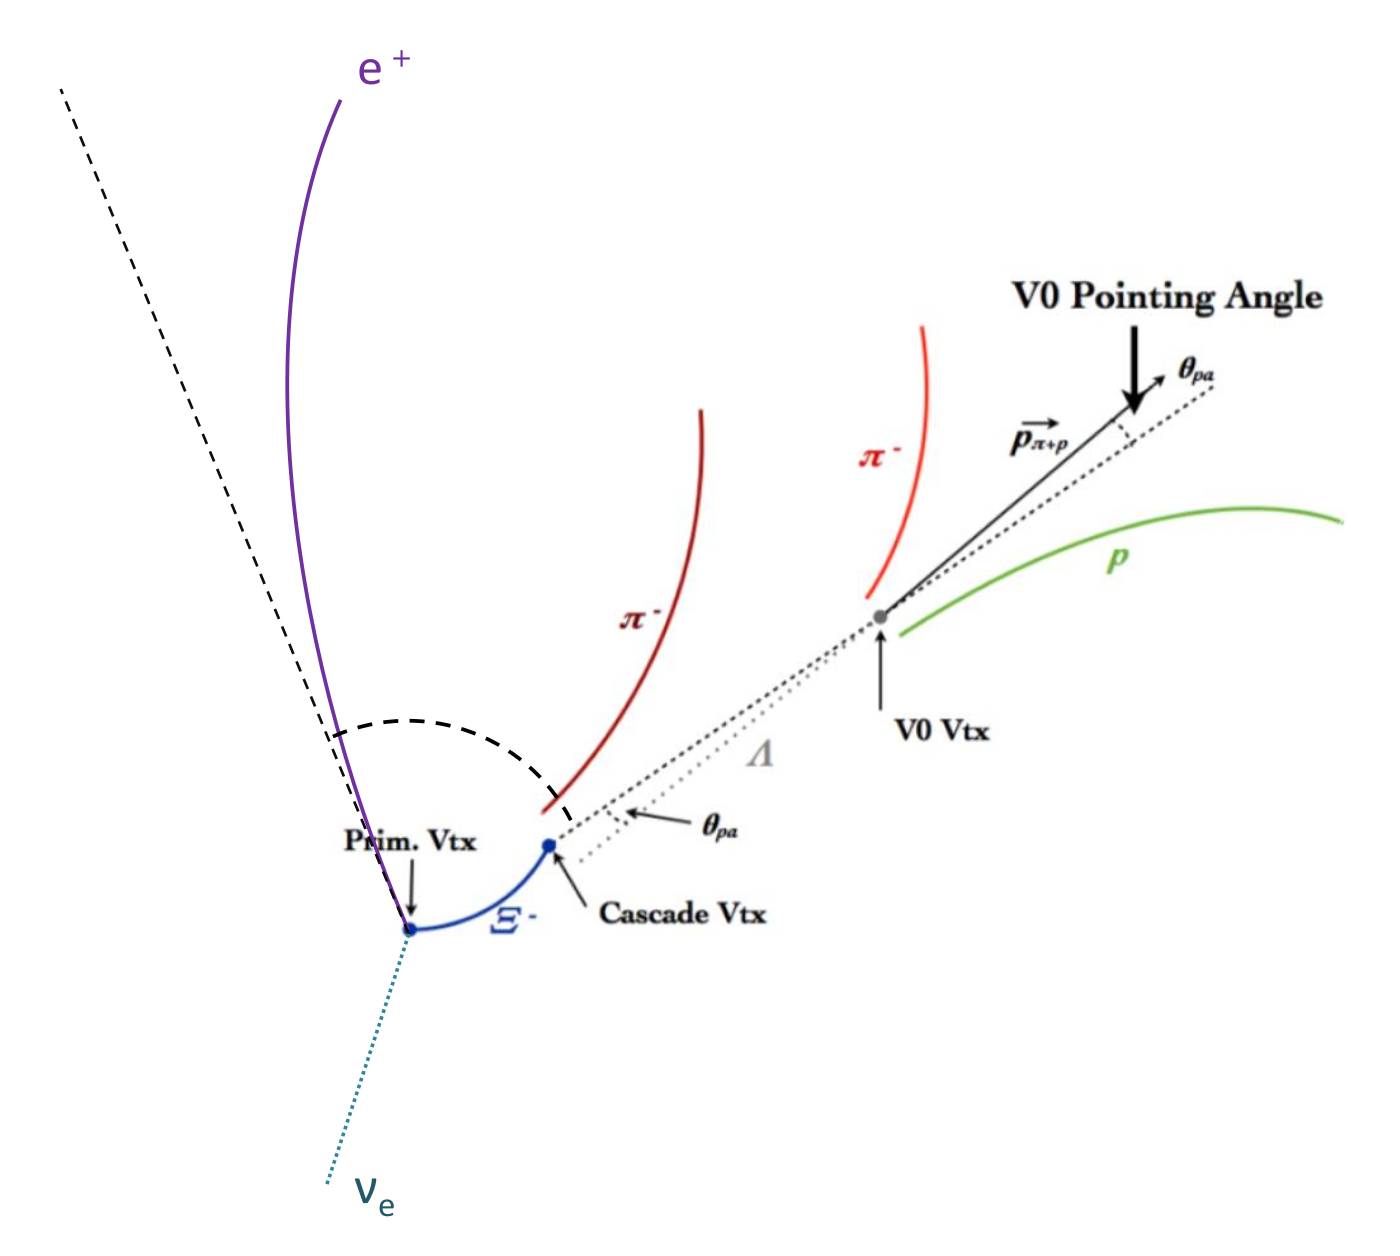
\includegraphics[width=0.50\textwidth]{plots/s2_strategy.png}
    \caption{Chain of \Xic $\rightarrow$ e\Xim decay}
    \label{fig:s2_decay}
\end{figure}

The strategy of measuring the \Xic can be summarized as follows.
%
\begin{itemize}
    \small
    \item[] \blue{Online event selection} \vspace{1pt}
    \item[-] Collect candidates of e-\Xim pair in loose conditions \vspace{\columnsep}
    \item[] \blue{Offline event selection} \vspace{1pt}
    \item[-] Apply eventwise cuts (e.g., sorting out by configuration)
    \item[-] Sort out candidates by quality (e.g., topology cut for \Xim) \vspace{\columnsep}
    \item[] \blue{Offline analysis} \vspace{1pt}
    \item[1.] Make e-\Xim pairs by charge sign: RS (right sign, sign is opposite to each other) or WS (wrong-sign), \\then obtain the signal distribution by RS - WS
    \item[2.] Correct efficiency for "prefilter" on electron candidates
    \item[3.] Correct the over-subtraction caused by \Xib
    \item[4.] Convert \pt of e-\Xim pair into \pt of \Xic by unfolding
    \item[5.] Correct efficiency for \Xic by using MC
    \item[6.] Correct for the prompt \Xic fraction
    \item[7.] Compute final observable
\end{itemize}
%
Further detailed information such as cut values can be found in the following section \ref{subsec:anaPrs}.





\clearpage
%--------------------------------------------------------

\subsection{Analysis process} \label{subsec:anaPrs}
\subsubsection{Online event selection} \label{subsubsec:onSel}
The conditions applied for the event selection via \textit{AliAnalysisTask} and ALICE \textit{Lego train} system are summarized in the following items. Note that the conditions are chosen very loosely, leaving fine filtering to the later offline event selection stage.

\begin{itemize}
    \small
    \item [] \blue{Eventwise cuts} \vspace{1pt}
    \item[-] 252000 $<$ run number
     \footnote{\textit{AliVEvent::GetRunNumber()}} $<$ 295000
     \item[-] Either MB or HMV0 trigger is fired
     \footnote{\textit{AliVEvent::kINT7, AliVEvent::kHighMultV0}}
     \item[-] Valid V0M multiplicity can be found
     \footnote{\textit{AliMultSelection::GetMultiplicityPercentile("V0M")}}
    \item[-] Primary vertex $|$z$|$ $<$ 10 (cm)
     \footnote{\textit{AliVVertex::GetZ()} $<$ 10.0}
    \item[-] Pileup rejection
     \footnote{\textit{AliRDHFCutsXictoeleXifromAODtracks::SetOptPileup(AliRDHFCuts::kRejectMVPileupEvent)}}
    %\item[-] Assign an \textit{AliNormalizationCounter} object for each configuration
\end{itemize}
%
\begin{itemize}
    \small
    \item[] \blue{Cuts for track (common)} \vspace{1pt}
    \item[-] AOD filter bit of 4 (standard cuts with very loose DCA)
    \footnote{\textit{AliAODTrack::TestFilterMask(AliAODTrack::kTrkGlobalNoDCA)}}
    % https://github.com/alisw/AliRoot/blob/master/STEER/AOD/AliAODTrack.h
    \item[-] \pt $>$ 0.5 (\GeVc) \footnote{\textit{AliAODTrack::Pt() $>$ 0.5)}}
    \item[-] $|\eta|$ $<$ 0.8 \footnote{\textit{AliAODTrack::Eta() $<$ 0.8}}
    \item[-] Number of TPC pID clusters $>$ 50
    \footnote{\textit{AliAODTrack::GetTPCsignalN() $>$ 50}}
    \item[-] Quality cuts
    \footnote{\textit{AliESDtrackCuts::SetClusterRequirementITS(AliESDtrackCuts::kSPD, AliESDtrackCuts::kBoth)}}
    \footnote{\textit{AliESDtrackCuts::SetDCAToVertex2D(true)}}
    \footnote{\textit{AliESDtrackCuts::SetMaxChi2PerClusterITS(36)}}
    \footnote{\textit{AliESDtrackCuts::SetMaxDCAToVertexXY(1.0)}}
    \footnote{\textit{AliESDtrackCuts::SetMaxDCAToVertexZ(2.0)}}
    \footnote{\textit{AliESDtrackCuts::SetMinNClustersITS(2)}}
    \footnote{\textit{AliESDtrackCuts::SetRequireTPCRefit(true)}}
    \footnote{\textit{AliESDtrackCuts::SetRequireITSRefit(true)}}
\end{itemize}
%
\begin{itemize}
    \small
    \item[] \blue{Cuts for cascade/V0 tracks} \vspace{1pt}
    \item[-] $|\sigma_{\rm TPC}| <$ 4
     \footnote{\textit{AliPIDResponse::NumberOfSigmasTPC() $<$ 4}}
    %\item[-] Reject charged $\Lambda$ %by mass tolerance of 0.008
    %\item[-] Valid decay lengths (both $\Xi$ and V0)
    \item[-] DCA of bachelor track to PV (primary vertex) $>$ 0.01 (cm)
     \footnote{\textit{AliAODcascade::DcaBachToPrimVertex()}}
    \item[-] DCA of V0 to PV $>$ 0.01 (cm)
     \footnote{\textit{AliAODcascade::DcaV0ToPrimVertex()}}
    \item[-] DCA of V0 daughters to PV $>$ 0.05 (cm)
     \footnote{\textit{AliAODcascade::Dca(Pos/Neg)ToPrimVertex()}}
    \item[-] (Both \Xim and V0) Daughters' DCA $<$ 1.68 (cm)
     \footnote{\textit{AliAODcascade::DcaXiDaughters(),
     AliAODcascade::DcaV0Daughters()}}
    \item[-] (Both \Xim and V0) Cosine of pointing angle $>$ 0.98
     \footnote{\textit{AliAODcascade::CosPointingAngle(),
     AliAODcascade::CosPointingAngleXi()}}
    \item[-] (Both \Xim and V0) Decay length $>$ 0.2 (cm)
     \footnote{Calculated from \textit{AliAODcascade::DecayVertex(Xi/V0)(X/Y/Z)}}
    \item[-] $\lambda$ mass tolerance: 0.008 (\GeVmass)
    \item[-] Reject \Omg baryon by mass
\end{itemize}
%
\clearpage
\begin{itemize}
    \small
    \item[] \blue{Cuts for electron track} \vspace{1pt}
    \item[-] Minimum \footnote{Minimum = {-4.3 + (1.17*\pt) - (0.094*\ensuremath{p_{\rm T^{2}}})},
    fix multiplied \pt to 5.0 if \pt $>$ 5.0} $< |\sigma_{\rm TPC}| <$ 3
    \item[-] $|\sigma_{\rm TOF}| <$ 3
     \footnote{\textit{AliPIDResponse::NumberOfSigmasTOF() $<$ 3}}
    \item[-] m$_{\,e^{+}e{-}}$ $<$ 0.05 (\GeVmass)
\end{itemize}
%

The total number of events processed during the online selection is summarized in table \ref{tab:nEvents}.
Note that the number of events was independently counted for each configuration by assigning an \textit{AliNormalizationCounter} object to each configuration. Also, the vertex finding efficiency was applied \footnote{\textit{AliNormalizarionCounter::GetNEventsForNorm()}} for the values.

\vspace{\columnsep}
\begin{table}[h]
    \centering
    \small
    \begin{tabular}{l|c|c|c}
    \hline\hline
    \multirow{2}{*}{Configuration} & \# of events ($B$) & \# of events ($B$) & Difference \\
    & (default) & (INEL$>$0) & ($|$default - INEL$>$0$|$ / default) \\\hline
    MB + [0, 100]   & 1.794 & 1.691 & 0.0574 \\\hline
    MB + [30, 100]  & 1.287 & 1.188 & 0.0769 \\\hline
    MB + [0.1, 30]  & 0.502 & 0.501 & 0.0020 \\\hline
    HMV0 + [0, 0.1] & 0.499 & 0.499 & 0.0000 \\
    \hline\hline
    \end{tabular}
    \caption{Total number of events processed for each configuration}
    \label{tab:nEvents}
\end{table}





\vspace{\columnsep}
%\clearpage
%--------------------------------------------------------
\subsubsection{Offline event selection} \label{subsubsec:offSel}
A ROOT file with Tree based structure is generated as a result of previous online event selection. The conditions applied to collect the e-\Xim pair candidates are summarized in the following item and tables \ref{tab:ePID} - \ref{tab:eXiPair}.
All selection conditions except the eventwise cuts are categorized in five levels by its tightness: vloose (very loose), loose, stand (standard), tight, and vtight, respectively. As the name indicates, stand is the default condition of the analysis.
Note that the offline selection performed independently by sample type and configuration (e.g., MB + [0, 100] for data). The weighting on generated \pt (section \ref{subsubsec:ptWeighting}) also performed at this stage.

\begin{itemize}
    \small
    \item [] \blue{Eventwise cuts (for each configuration)} \vspace{1pt}
    \item[-] Target trigger is fired (e.g., MB)
    \item[-] V0M multiplicity is within the range (e.g., 0.1 $<$ multiplicity percentile $<$ 30)
    \item[-] INEL$>$0
    \item[-] electron mass $>$ 0.05 (\GeVmass)
    \item[-] $\Xi$ mass tolerance: $\pm$ 0.008 (\GeVmass)
    %\item[-] $\Xi$ mass within tolerance: 1.32171 $\pm$ 0.008 (\GeVmass)
    \item[-] e-$\Xi$ pair mass $>$ 1.3 (\GeVmass)
    \footnote{\textit{AliPPVsMultUtils::IsINELgtZERO(AliVEvent)}}
    %\footnote{MC: \textit{AliAODMCParticle::IsPhysicalPrimary() \&\& Charge() != 0 \&\& $|\eta|$ $<$ 1.0}}
\end{itemize}

\vspace{\columnsep}
\begin{table}[hb]
    \centering
    \small
    \begin{tabular}{r|c|c|c}
    \hline\hline
    %ut (level\textbackslash item) & $\sigma_{\rm TPC}$ min ($\geq$) & $\sigma_{\rm TPC}$ max ($\leq$) & $|\sigma_{\rm TOF}|$ ($\leq$) \\\hline
    \multirow{2}{*}{Cut (level\textbackslash item)} & $\sigma_{\rm TPC}$ min ($\geq$) & 
    \multirow{2}{*}{$\sigma_{\rm TPC}$ max ($\leq$)} & 
    \multirow{2}{*}{$|\sigma_{\rm TOF}|$ ($\leq$)} \\
    & * Variable \pt is fixed to 5.0 if \pt $>$ 5.0 & & \\\hline
    vloose & {-4.3 + (1.17*\pt) - (0.094*\ensuremath{p_{\rm T^{2}}})} & \multirow{5}{*}{3} & \multirow{5}{*}{3} \\\cline{1-2}
    loose  & {-4.1 + (1.17*\pt) - (0.094*\ensuremath{p_{\rm T^{2}}})} & & \\\cline{1-2}
    stand  & {-3.9 + (1.17*\pt) - (0.094*\ensuremath{p_{\rm T^{2}}})} & & \\\cline{1-2}
    tight  & {-3.7 + (1.17*\pt) - (0.094*\ensuremath{p_{\rm T^{2}}})} & & \\\cline{1-2}
    vtight & {-3.5 + (1.17*\pt) - (0.090*\ensuremath{p_{\rm T^{2}}})} & & \\
    \hline\hline
    \end{tabular}
    \caption{Table of cuts for electron pID in offline selection%. The variable \pt being multiplied in the column $\sigma_{\rm TPC}$ min is fixed to 5.0 if the \pt $>$ 5.0
    }
    \label{tab:ePID}
\end{table}
%
\begin{table}[ht]
    \centering
    \small
    \begin{tabular}{l|c|c|c|c|c}
    \hline\hline
    Cut (item\textbackslash level) & vloose & loose & stand & tight & vtight \\\hline
    \# of crossed rows ($>$)                        & 65 & 65 & 70 & 75 & 85 \\\hline
    \# of TPC pID clusters ($>$)                    & 40 & 45 & 50 & 55 & 60 \\\hline
    \# of crossed rows/\# of TPC pID clusters ($>$) & 0.70 & 0.75 & 0.80 & 0.85 & 0.90 \\\hline 
    \# of ITS clusters ($\geq$)                     & \multicolumn{5}{c}{3} \\
    \hline\hline
    \end{tabular}
    \caption{Table of cuts for electron reconstruction in offline selection}
    \label{tab:eReco}
\end{table}
%
\begin{table}
    \centering
    \small
    \begin{tabular}{l|c|c|c|c|c}
    \hline\hline
    Cut (item\textbackslash level) & vloose & loose & stand & tight & vtight \\\hline
    Decay length of \Xim (cm) ($>$)         & 0.5 & 0.5 & 0.5 & 0.6 & 0.7 \\\hline
    Decay length of V0 (cm) ($>$)           & 1.10 & 1.55 & 2.67 & 3.60 & 4.39 \\\hline
    DCA of bachelor track to PV (cm) ($>$)  & 0.05 & 0.05 & 0.07 & 0.09 & 0.11 \\\hline
    DCA of V0 to PV (cm) ($>$)              & 0.05 & 0.07 & 0.09 & 0.10 & 0.12 \\\hline
    DCA of V0 daughters to PV (cm) ($>$)    & 0.05 & 0.07 & 0.095 & 0.11 & 0.13 \\\hline
    Cosine of pointing angle (both \Xim and V0) ($>$) & 0.98 & 0.981 & 0.983 & 0.9839 & 0.985 \\
    \hline\hline
    \end{tabular}
    \caption{Table of cuts for \Xim pID by topology in offline selection}
    \label{tab:XiPID}
\end{table}
%
\begin{table}
    \centering
    \small
    \begin{tabular}{l|c|c|c|c|c}
    \hline\hline
    Cut (item\textbackslash level) & vloose & loose & stand & tight & vtight \\\hline
    \# of crossed rows (V0 proton) ($>$) & \multirow{3}{*}{66} & \multirow{3}{*}{66} &
    \multirow{3}{*}{70} & \multirow{3}{*}{70} & \multirow{3}{*}{74} \\
    \# of crossed rows (V0 \ensuremath{\pi}\xspace) ($>$) & & & & & \\
    \# of crossed rows (cascade \ensuremath{\pi}\xspace) ($>$) & & & & & \\\hline
    \# of crossed rows/findable (V0 proton) ($>$) & \multirow{3}{*}{0.74} & \multirow{3}{*}{0.77} & \multirow{3}{*}{0.77} & \multirow{3}{*}{0.79} & \multirow{3}{*}{0.79} \\
    \# of crossed rows/findable (V0 \ensuremath{\pi}\xspace) ($>$) & & & & & \\
    \# of crossed rows/findable (cascade \ensuremath{\pi}\xspace) ($>$) & & & & & \\
    \hline\hline
    \end{tabular}
    \caption{Table of cuts for \Xim reconstruction in offline selection}
    \label{tab:XiReco}
\end{table}
%
\begin{table}[hb]
    \centering
    \small
    \begin{tabular}{l|c|c|c|c|c}
    \hline\hline
    Cut (item\textbackslash level) & vloose & loose & stand & tight & vtight \\\hline
    Mass (\GeVmass) ($<$) & N/A & 2.7 & 2.5 & 2.3 & N/A \\\hline
    Opening angle (\degree) ($>$) & N/A & N/A & 90 & 70 & N/A \\
    \hline\hline
    \end{tabular}
    \caption{Table of cuts for e-\Xim pair in offline selection}
    \label{tab:eXiPair}
\end{table}





\clearpage
%--------------------------------------------------------
\subsubsection{Offline analysis} \label{subsubsec:offAna}
This section shows a series of analysis routines to reach the desired observable. Although the final physics observable of the analysis is the baryon-to-meson ratio by \Xic/\Dzero, the desired observable of this section is the corrected invariant cross-section of the \Xic, as we rely on existing result for \Dzero.

Note that only the plots for configuration MB + [0, 100] will be presented as an example: check appendix \ref{sec:appB} for other configurations.

\vspace{\columnsep}
\paragraph{\blue{Signal extraction by RS-WS}}\mbox{}\\[1pt]
The mass of \Xic is 2470.91 $\pm$ 0.25 (\MeVmass) \cite{PDG}, however, due to the presence of neutrino in this decay mode (\Xic $\rightarrow$ e$\Xi \nu_{e}$) one cannot expect to observe a distinct mass peak, 
thus the conventional signal yields extraction by using the peak cannot be used. As an alternative, we depend on the sign of e\Xim pair, by subtracting the WS (Wrong Sign, charge sign of e = \Xim) distribution from the RS (Right Sign, e $\neq$ \Xim).

Fig. \ref{fig:s2_RSWS} shows the distribution of RS/WS pairs by \pt bin and the resulting signal distribution by RS-WS. As the distributions show, the statistics are in general poor for \pt $>$ 8, and very scarce for \pt $>$ 12.

\vspace{\columnsep}
\begin{figure}[h!]
    \centering
    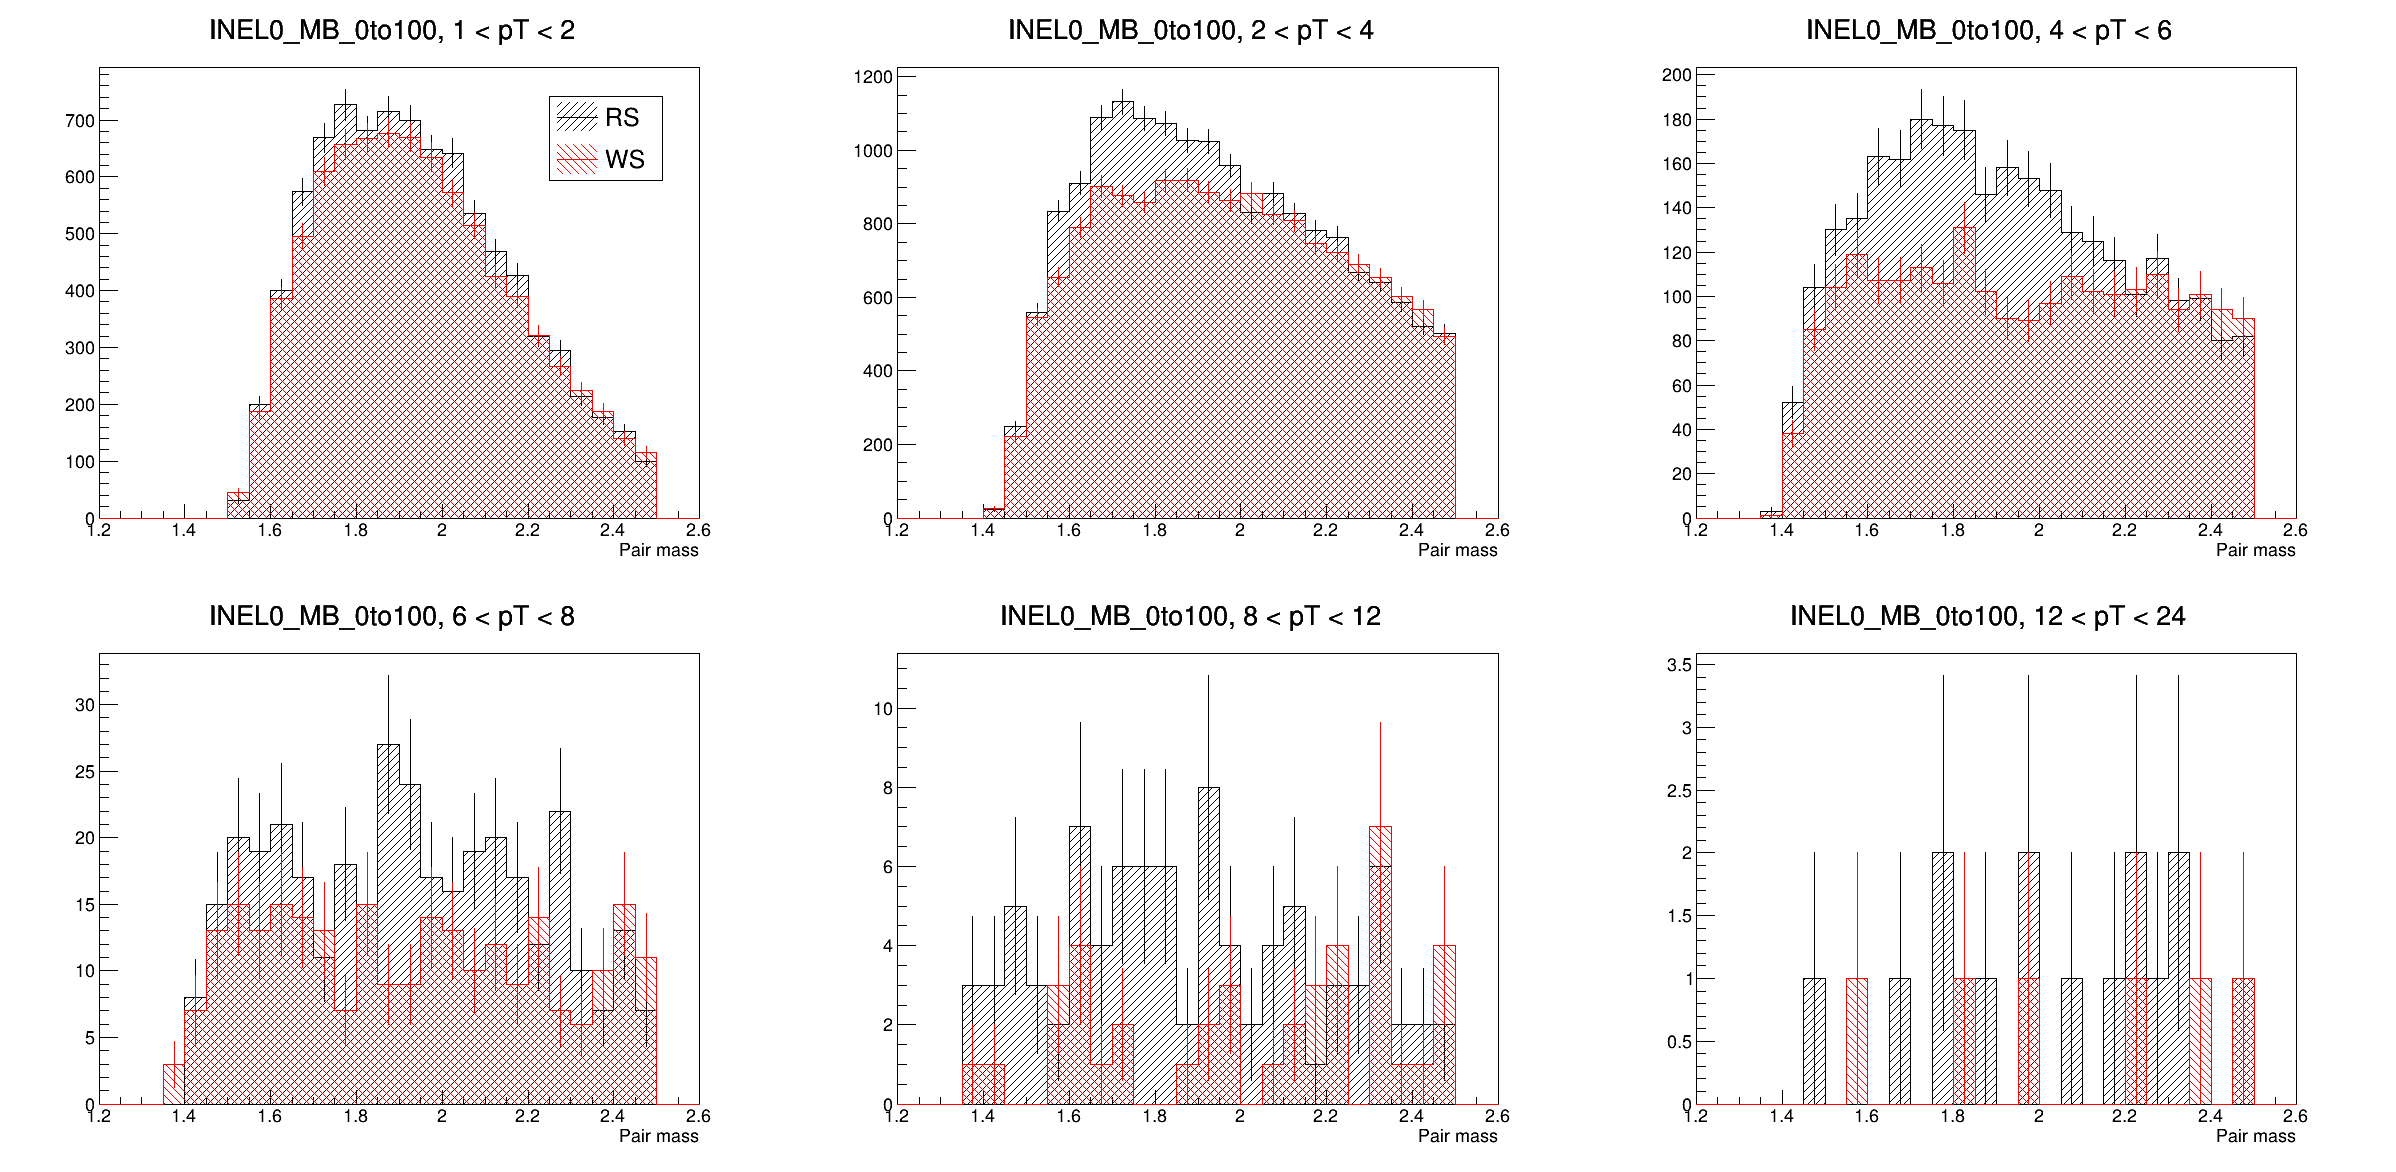
\includegraphics[width=0.90\textwidth]{plots/s2_RSmWS_INEL0_MB_0to100.png} \\\vspace{2pt}
    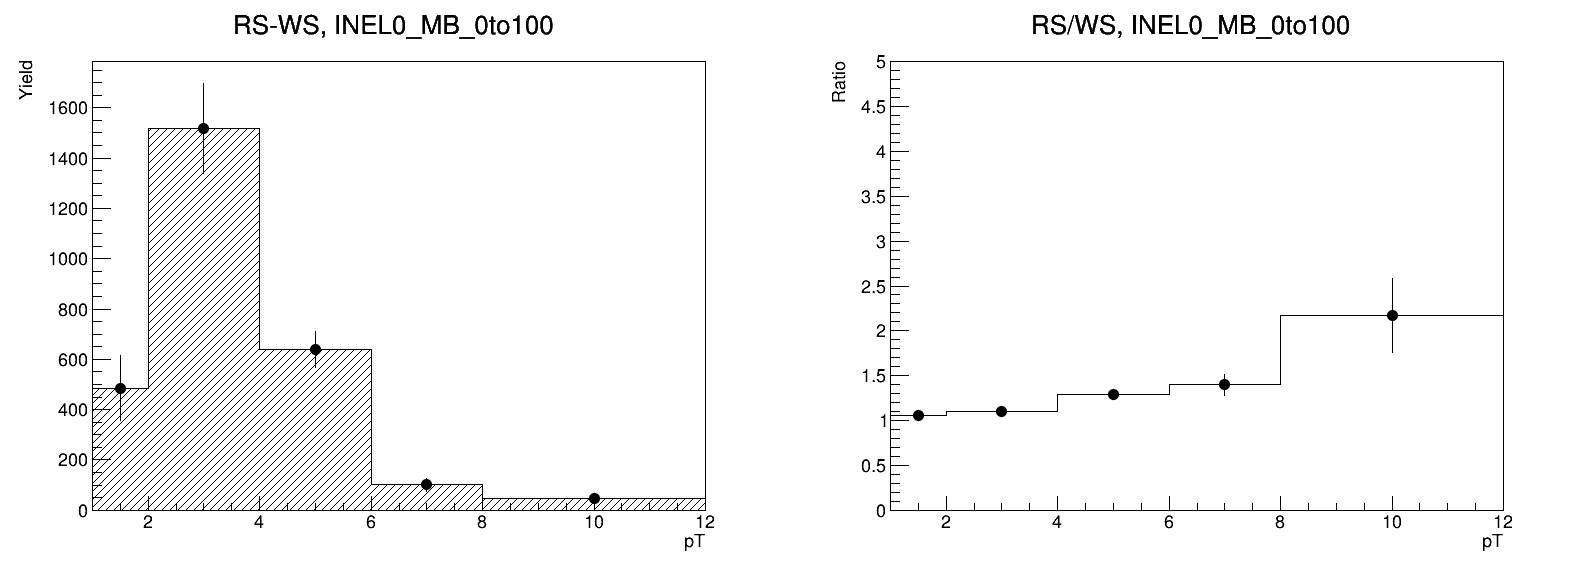
\includegraphics[width=0.95\textwidth]{plots/s2_RSdWS_INEL0_MB_0to100.png}
    \caption{\pt distributions of e\Xim pairs by sign (RS or WS) (top 6), extracted signal by RS-WS (bottom left), and ratio of RS/WS (bottom right). Only the configuration MB + [0, 100] is shown.}
    \label{fig:s2_RSWS}
\end{figure}

\clearpage
%++++++++++++++++++++++++++++++++++++++++++++

\vspace{\columnsep}
\paragraph{\blue{Prefilter efficiency correction}}\mbox{}\\[1pt]
A portion of signal electrons can be accidentally rejected by the applied electron track selection cuts (prefilter) during the online event selection. The definition of prefilter efficiency for the correction is as follows.

\begin{equation}
    \epsilon_{\,\text{\rm prefilter}} =
    \frac{N_{e\Xim} \text{\rm \,(prefilter on, same-sign pairs)}}{N_{e\Xim} \text{\rm \,(prefilter off})}
\end{equation}

The numerator indicates the number of e\Xim pairs collected with prefilter applied while the denominator is not. Also, for the numerator, the backgrounds yields (e-\Xim pairs with the same sign) were utilized to prevent large fluctuation from the poor statistics of signals (e-\Xim pairs with different signs).

Fig. \ref{fig:s2_preFEff} shows the estimated prefilter efficiency and the signal yields before and after the correction.

\vspace{\columnsep}
\begin{figure}[h]
    \centering
    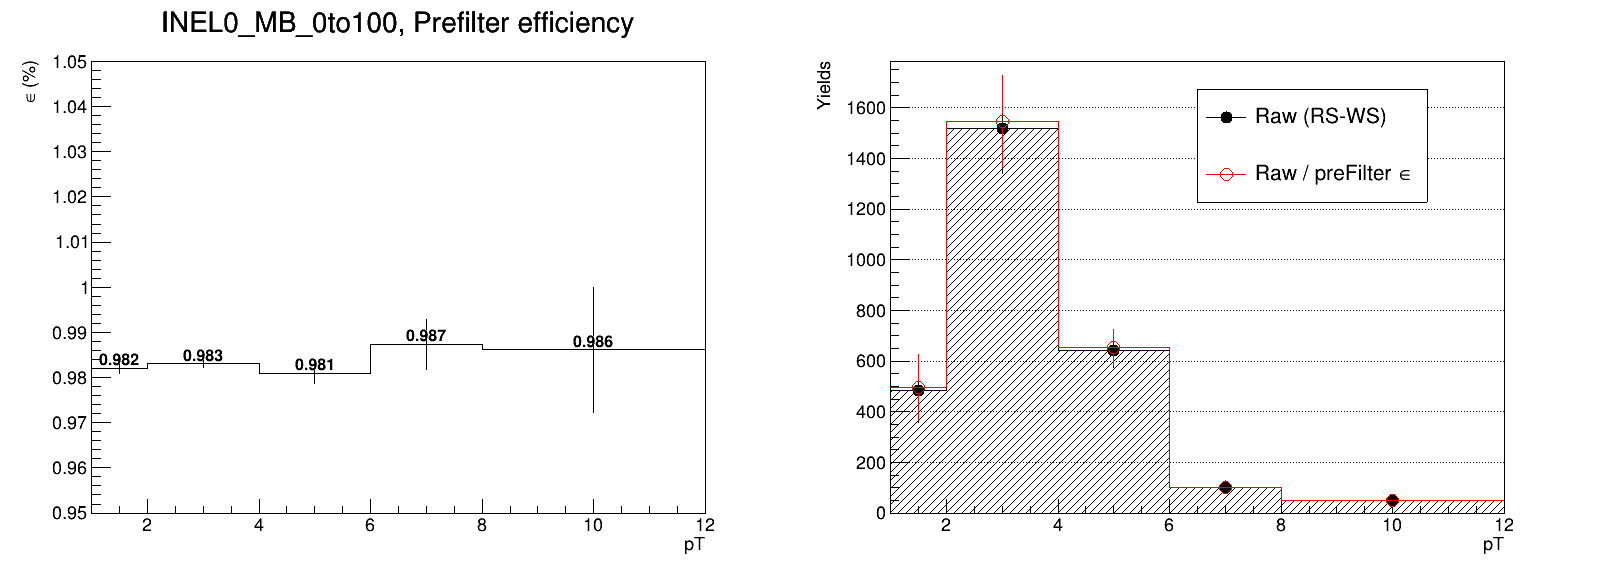
\includegraphics[width=0.95\textwidth]{plots/s2_preFCorr_INEL0_MB_0to100.png}
    \caption{Prefilter efficiency (left) and (RS-WS) yields before and after the correction (right)}
    \label{fig:s2_preFEff}
\end{figure}

%++++++++++++++++++++++++++++++++++++++++++++

\clearpage
\paragraph{\blue{\Xib over-subtraction correction}}\mbox{}\\[1pt]
\red{TBU}

\iffalse
- Uses 7 TeV CMS Lb \\
- Scale it up (7 $\rightarrow$ 13 TeV) by using FONLL\_B \\
- Normalize by using \# of events (normalization factor) and "V0 detector cross-section" \\
  (* V0 xSec is estimated for inclusive MB: would the xSec valid for HMV0 or specific mult. percentile?) \\
- Estimate efficiency of Xib (Xib generated vs. Xib reco) by using MC \\
  (* problem 1: Xib\_gen is prepared in train level) \\
  (* problem 2: Xib\_reco affected by the applied MC scaling factor (MB+[0, 100] != HMV0+[0,0.1]))
- Syst. err: cut tightness (std vs. vtight : applies to the Xib\ reco) \\
\fi
%
\begin{figure}[h]
    \centering
    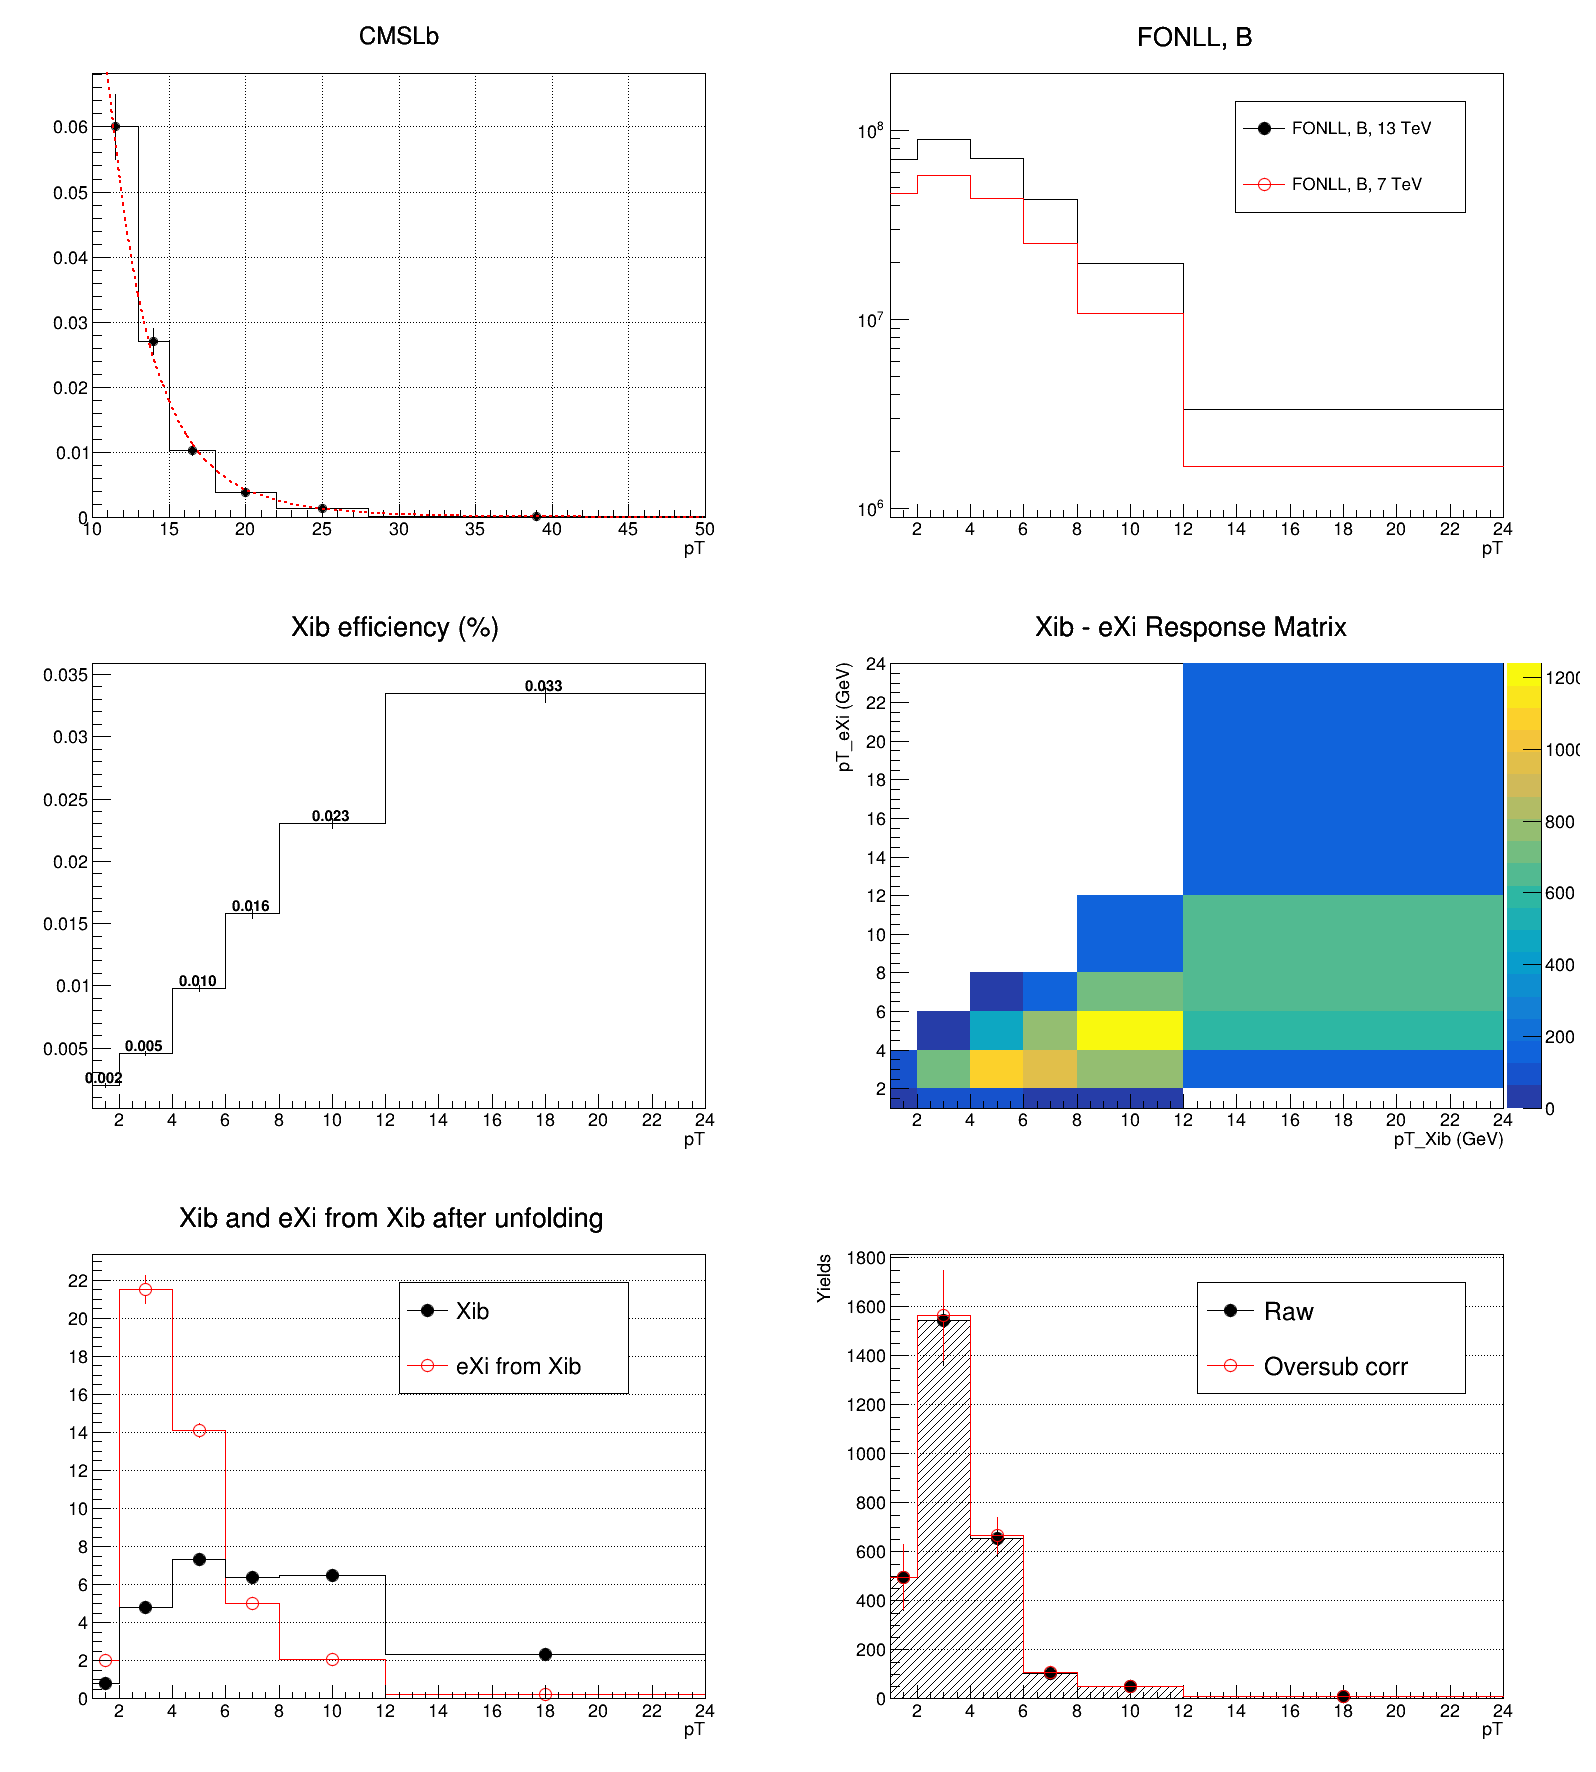
\includegraphics[width=0.95\textwidth]{plots/s2_c1b_Bayes_stand3_INEL0_MB_0to100_bCorr.png}
    \caption{\red{TBU}}
    \label{fig:s2_bCorr}
\end{figure}

\clearpage
%++++++++++++++++++++++++++++++++++++++++++++

\vspace{\columnsep}
\paragraph{\blue{Unfolding}}\mbox{}\\[1pt]
The unfolding can be explained as 'rewinding the distortion on the signal' by using truth information based on MC. By using the well-defined MC sample (PYTHIA8) and the same reconstruction process between the data and MC, the following relationship can be established between the measured quantity \textit{M} and the true quantity \textit{T}.

\vspace{\columnsep}
\centerline{\textit{M} = \textit{R} * \textit{T}}

The quantity \textit{R} is the Response Matrix of the detector which reflects the discrepancy between \textit{M} and \text{T} for given conditions (e.g., detector acceptance, etc). Note that the default method of the unfolding is Bayesian combined with an iterative procedure.

The subject variable of the unfolding is the \pt of the \Xic. Since the decay mode (\Xic $\rightarrow$ $e\Xi\nu_{e}$) includes a neutrino which cannot be measured with ALICE detectors, the unfolding is inevitably required to convert the measured e-\Xim pair's \pt to the one of \Xic.

Fig. \ref{fig:s2_unfolding} shows the applied Response Matrix and the yields before and after the unfolding.

\vspace{\columnsep}
\begin{figure}[h]
    \centering
    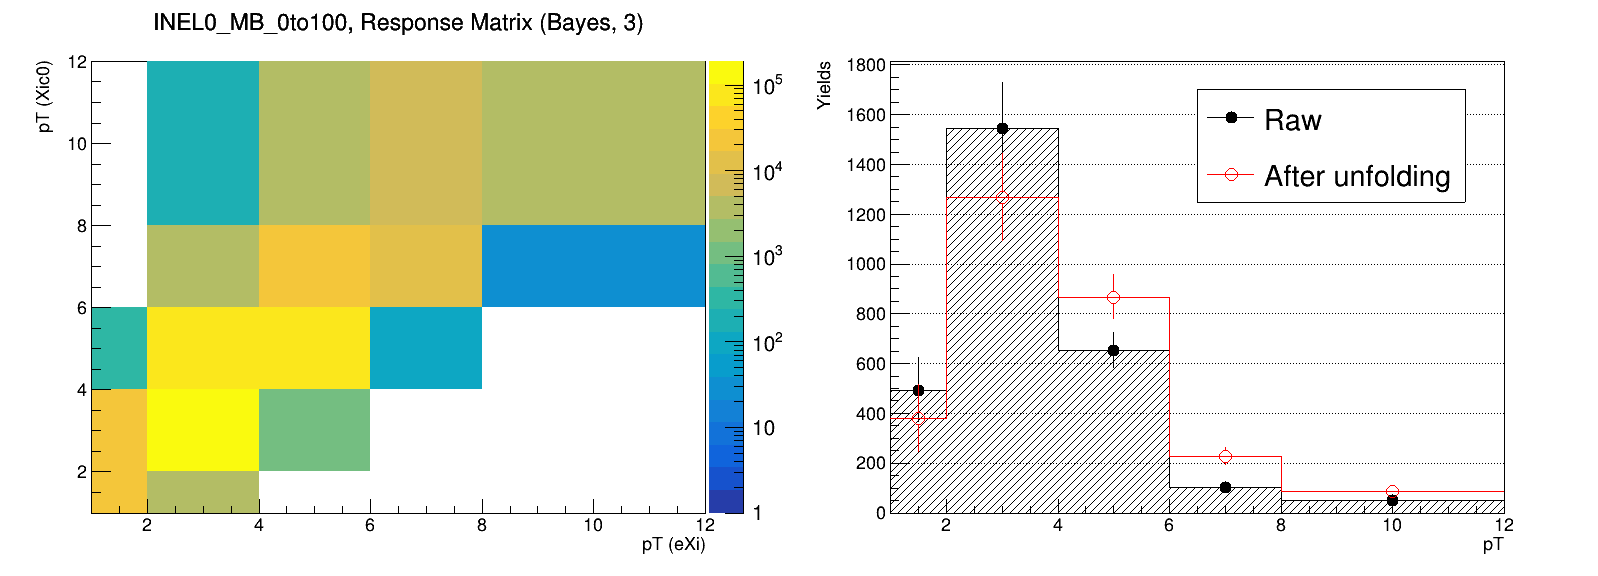
\includegraphics[width=0.95\textwidth]{plots/s2_unfold_INEL0_MB_0to100.png}
    \caption{\Xic - e\Xim response matrix by MC (left) and yields before and after the unfolding (right)}
    \label{fig:s2_unfolding}
\end{figure}

\clearpage
%++++++++++++++++++++++++++++++++++++++++++++

\vspace{\columnsep}
\paragraph{\blue{\Xic efficiency correction}}\mbox{}\\[1pt]
\red{TBU} \\

\begin{figure}[h]
    \centering
    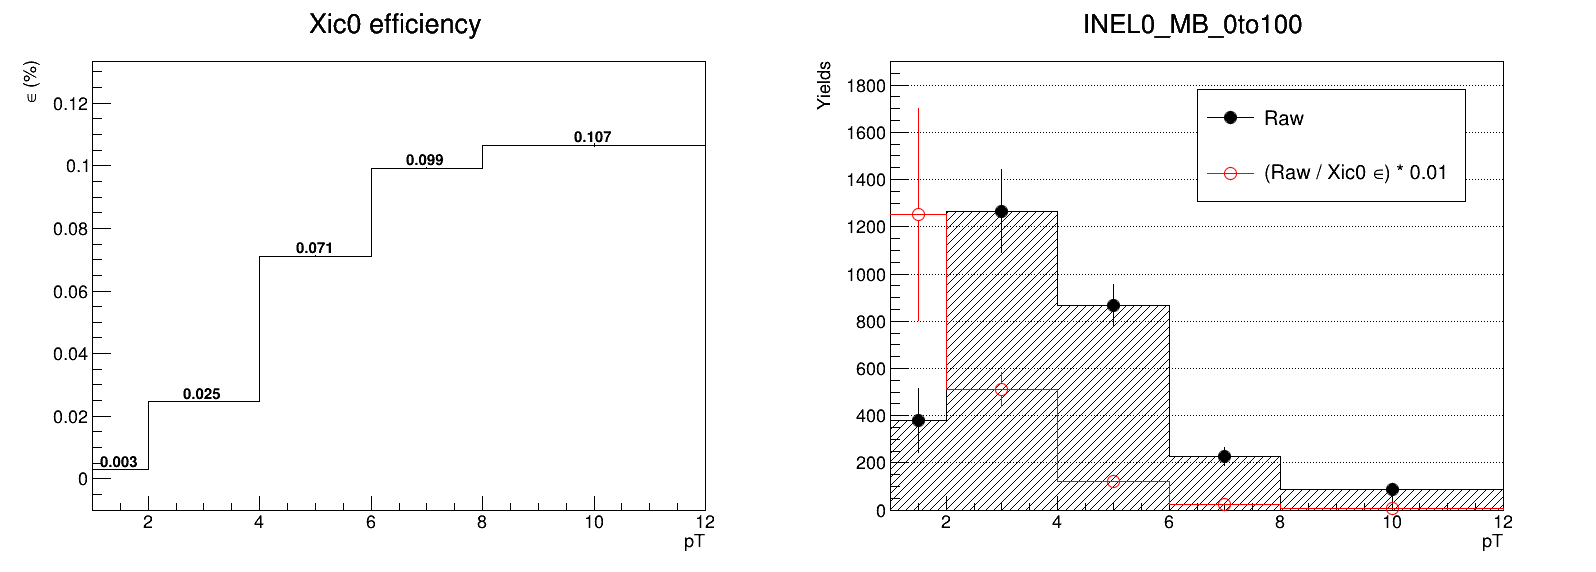
\includegraphics[width=0.95\textwidth]{plots/s2_Xic0Eff_INEL0_MB_0to100.png}
    \caption{$Acc \times \epsilon$ of \Xic (left) and Yields before and after correction (right)}
    \label{fig:s2_Xic0Eff}
\end{figure}

%\clearpage
%++++++++++++++++++++++++++++++++++++++++++++

\paragraph{\blue{Feed-down subtraction}}\mbox{}\\[1pt]
\red{TBU}

%\clearpage
%++++++++++++++++++++++++++++++++++++++++++++

\paragraph{\blue{Compute the yields}}\mbox{}\\[1pt]
\red{TBU}

\clearpage
%--------------------------------------------------------

\subsubsection{Crosscheck with previous analysis results} \label{subsubsec:xCheck}
%
As mentioned earlier in section \ref{sec:recap}, this analysis follows almost same analysis strategy by the previous \Xic $\rightarrow$ e\Xim analysis for \pp 13 \TeV. To ensure the validity of this study in addition to crosscheck the previous result, the overall analysis processes were cross-checked step by step, and then directly compared by using \Xic cross-section.
%
\begin{itemize}
    \small
    \item [] \blue{Crosscheck conditions} \vspace{1pt}
    \item[-] Target: MB inclusive (no multiplicity selection) \Xic cross-section
    \item[-] Online event selection: shared same Lego train output (section \ref{subsec:dataset}) \vspace{1pt}
    \item[-] Offline event selection: \\
     1. Uses each analyzer's codes \\
     2. Same cuts and factors (e.g., weighting factor for \pt spectra of MC) \vspace{1pt}
    \item[-] Offline analysis: \\
     1. Uses each analyzer's codes \\
     2. Same cuts and factors (e.g., Xic $\rightarrow$ e\Xim branching ratio) \\
     3. Same analysis steps (section \ref{subsubsec:onSel} - \ref{subsubsec:offAna}) are applied
\end{itemize}
%
The results of crosscheck are shown in Fig. \ref{fig:s2_xCheck}. The maximum deviation is smaller than 0.5 \%. Note that some factors applied are not necessarily the final one (e.g., Weighting factor for \pt spectra of MC) and among the analysis routines Feed-down subtraction was not applied.

\vspace{\columnsep}
\begin{figure}[h]
    \centering
    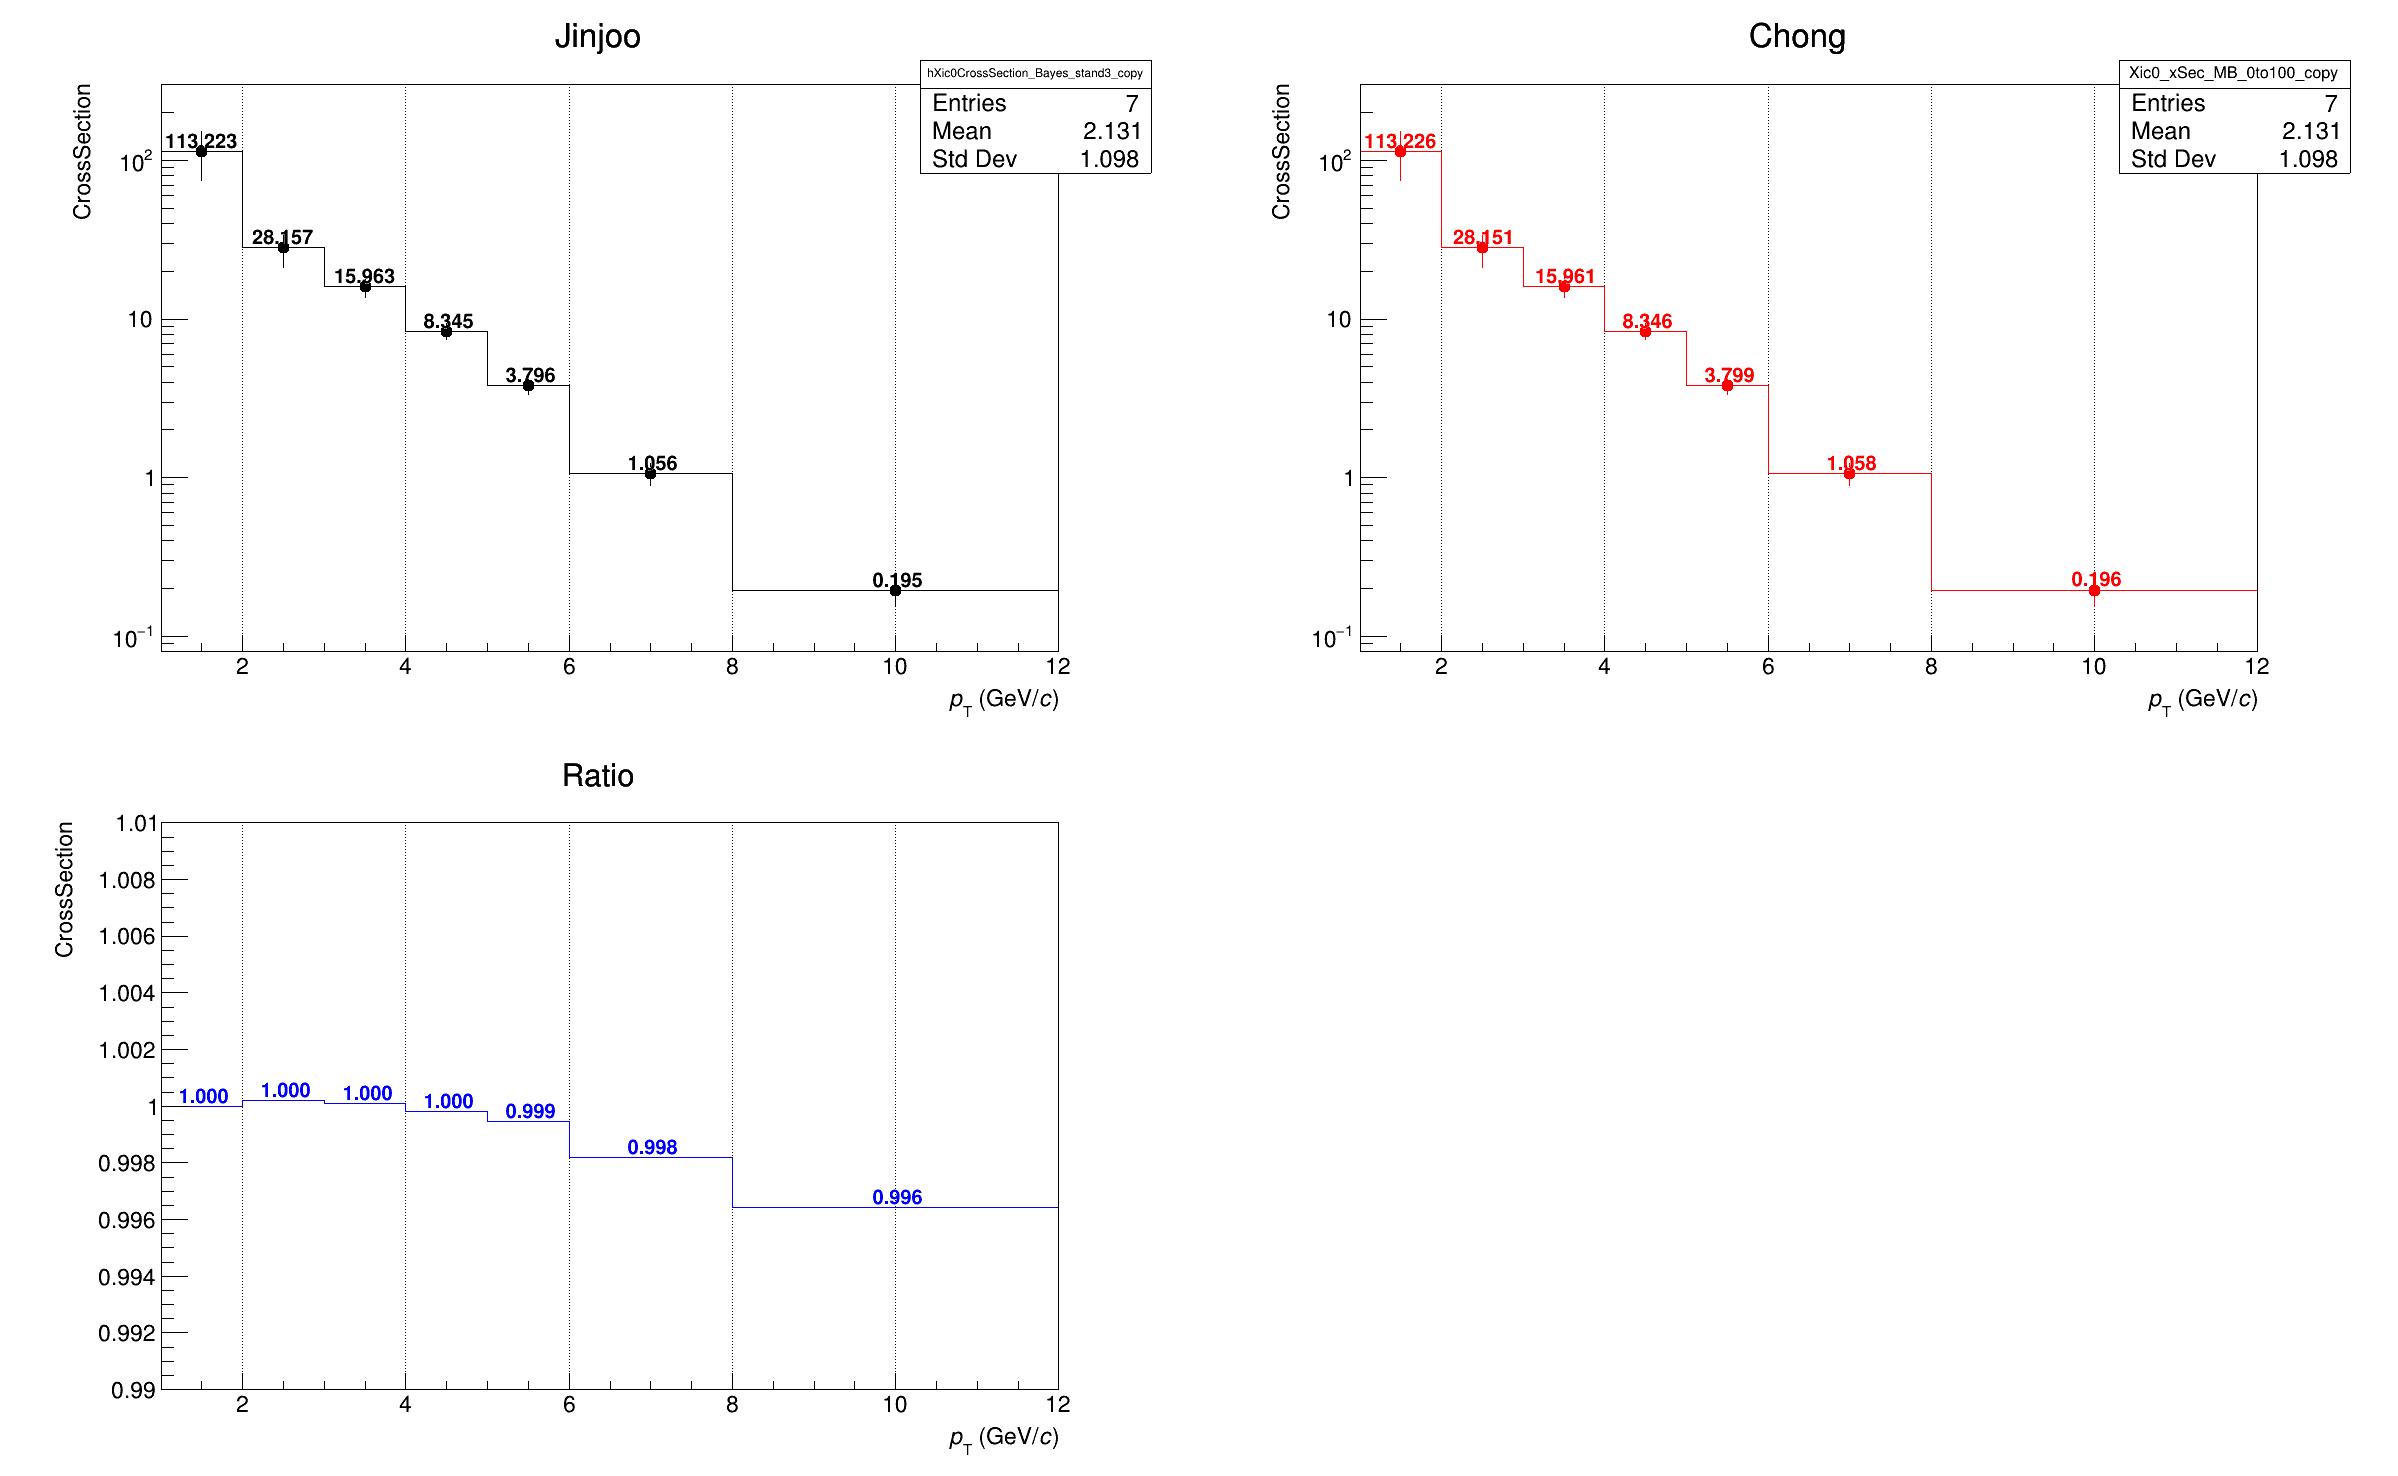
\includegraphics[width=0.95\textwidth]{plots/s2_xCheck.png}
    \caption{The crosscheck results: top left plot shows the \Xic cross-section by previous analysis, top right plot shows the same observable by this analysis, and bottom left shows the ratio between the them.}
    \label{fig:s2_xCheck}
\end{figure} \clearpage
\clearpage
\subsection{Studies and Updates} \label{subsec:update}

%-----------------------------------------------
\subsubsection{Weighting on generated \pt shape} \label{subsubsec:ptWeighting}
\red{TBU}

\begin{figure}[t]
    \centering
    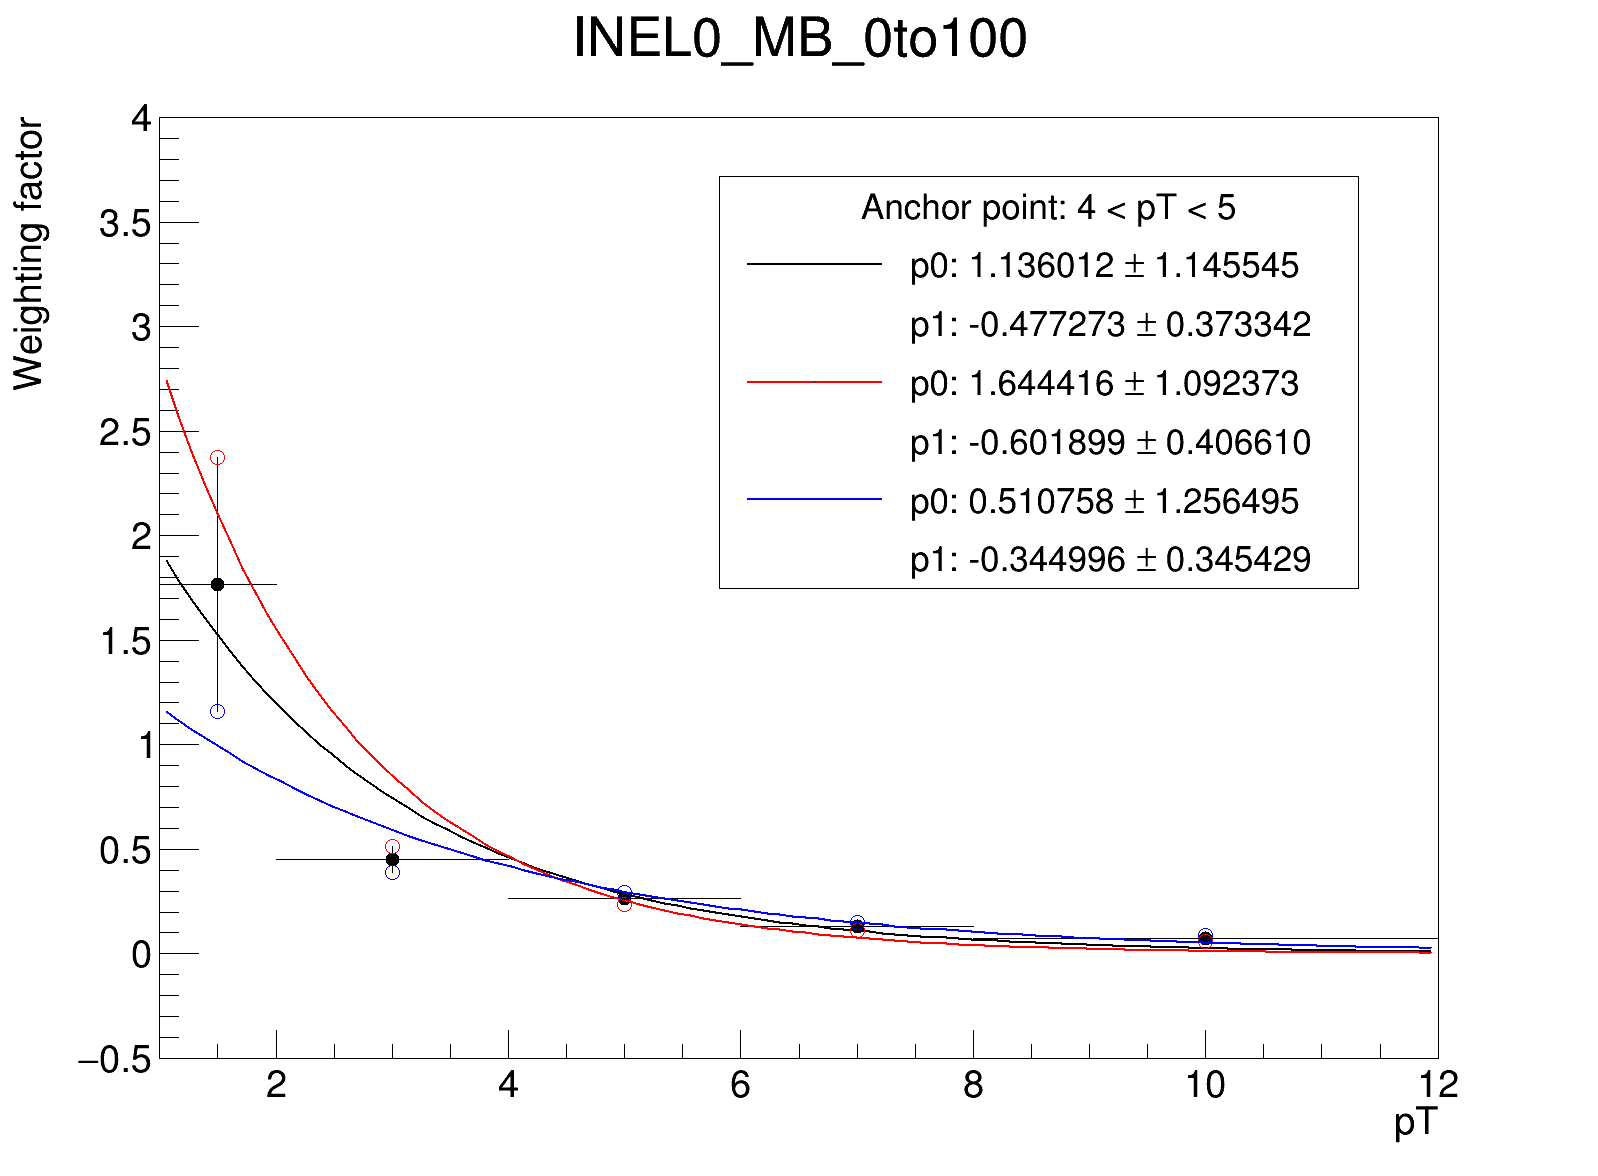
\includegraphics[width=0.45\textwidth]{plots/s2_pTW1to12_INEL0_MB_0to100.png}
    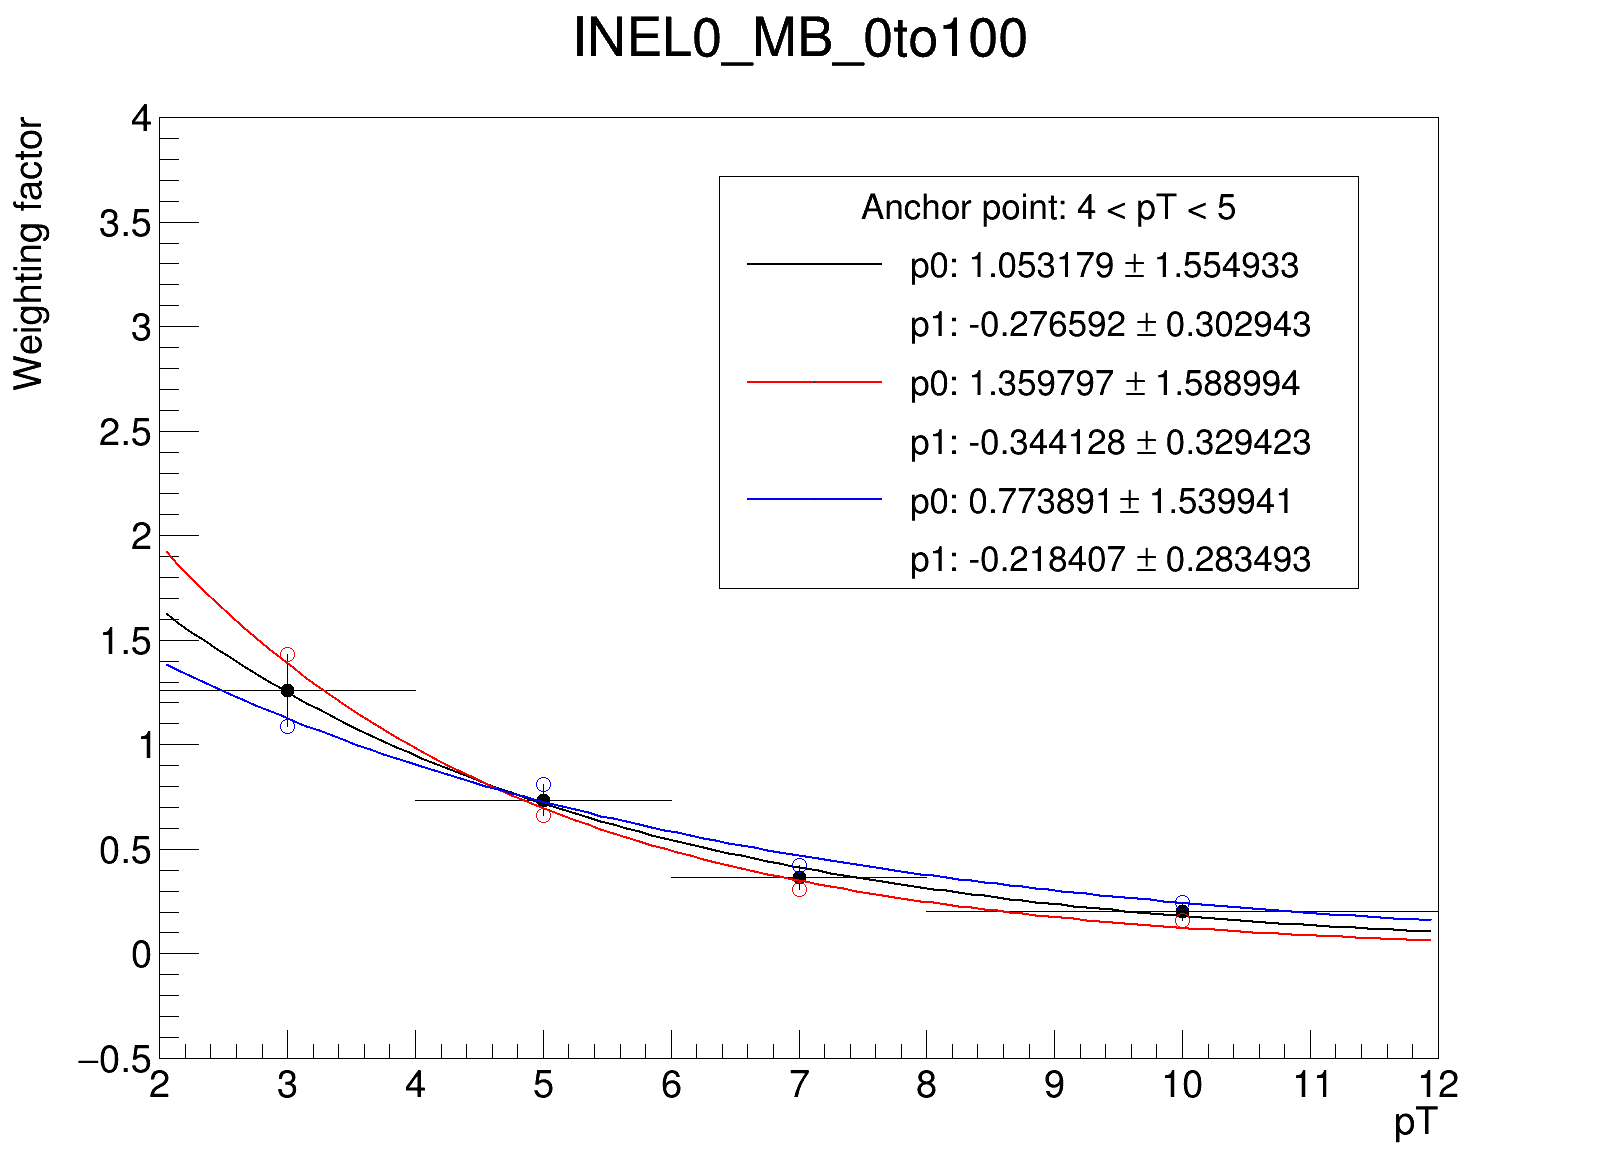
\includegraphics[width=0.45\textwidth]{plots/s2_pTW2to12_INEL0_MB_0to100.png}
    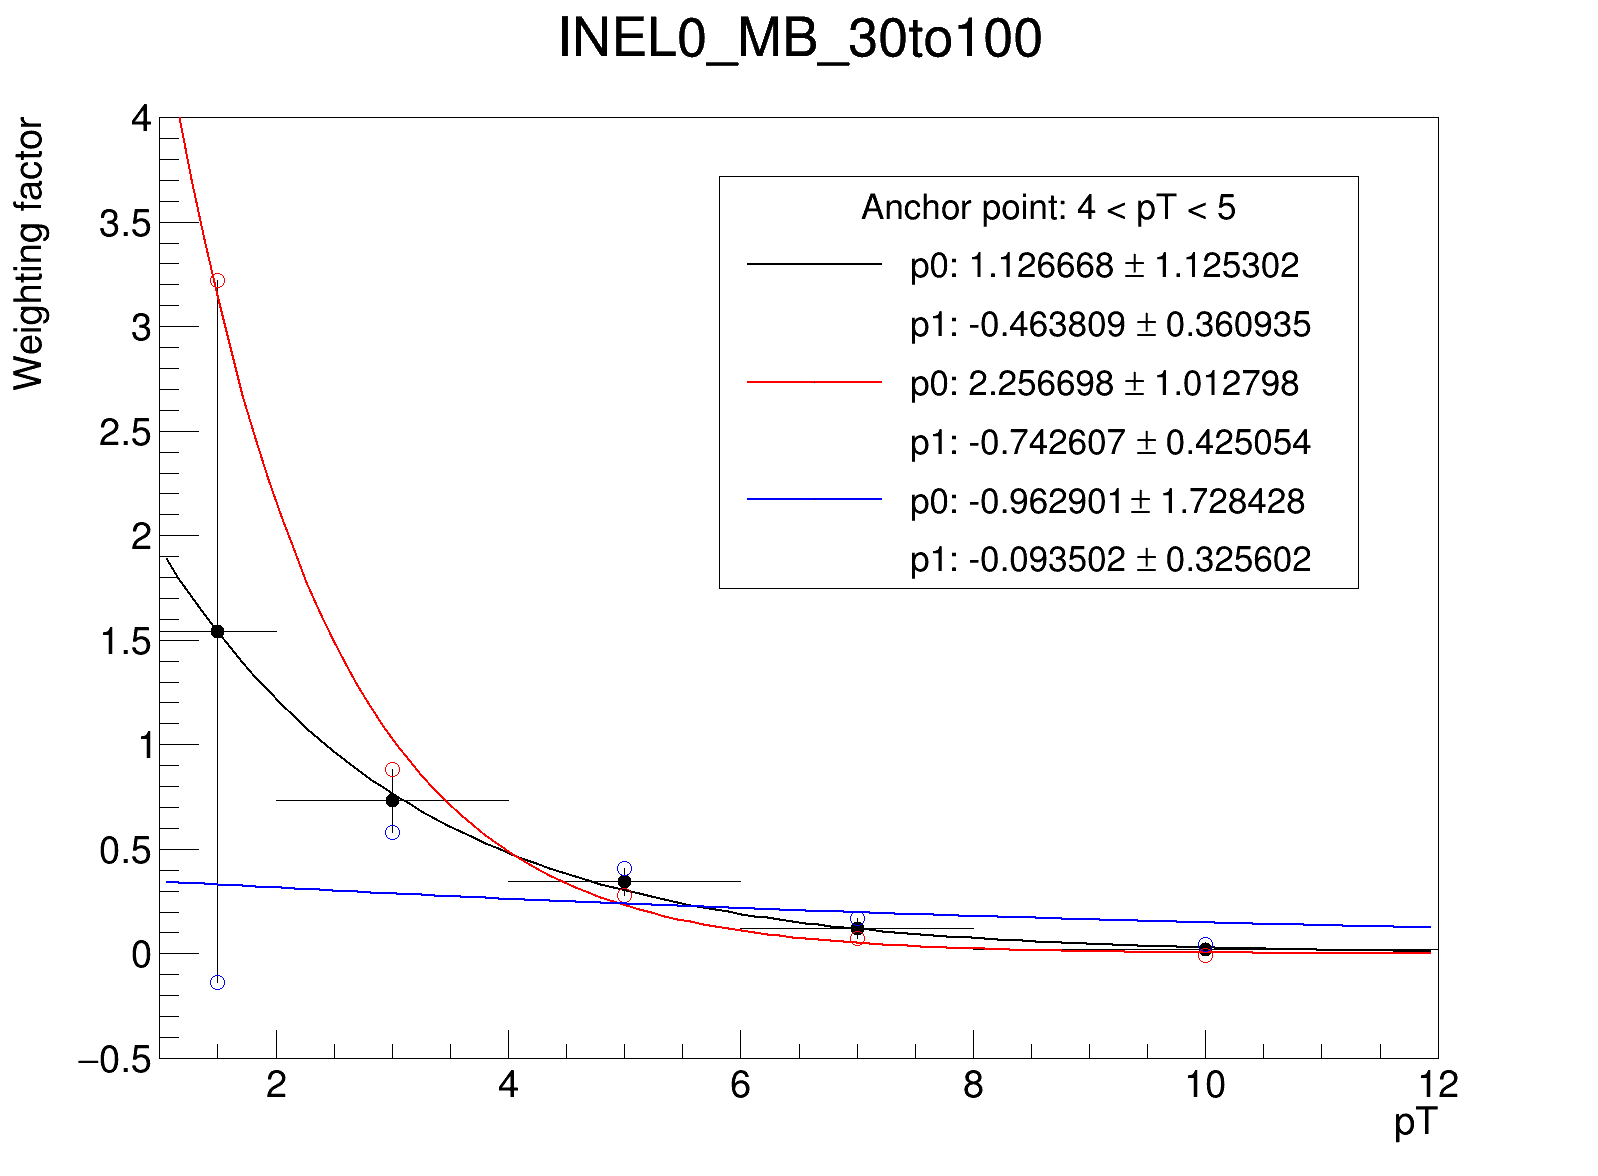
\includegraphics[width=0.45\textwidth]{plots/s2_pTW1to12_INEL0_MB_30to100.png}
    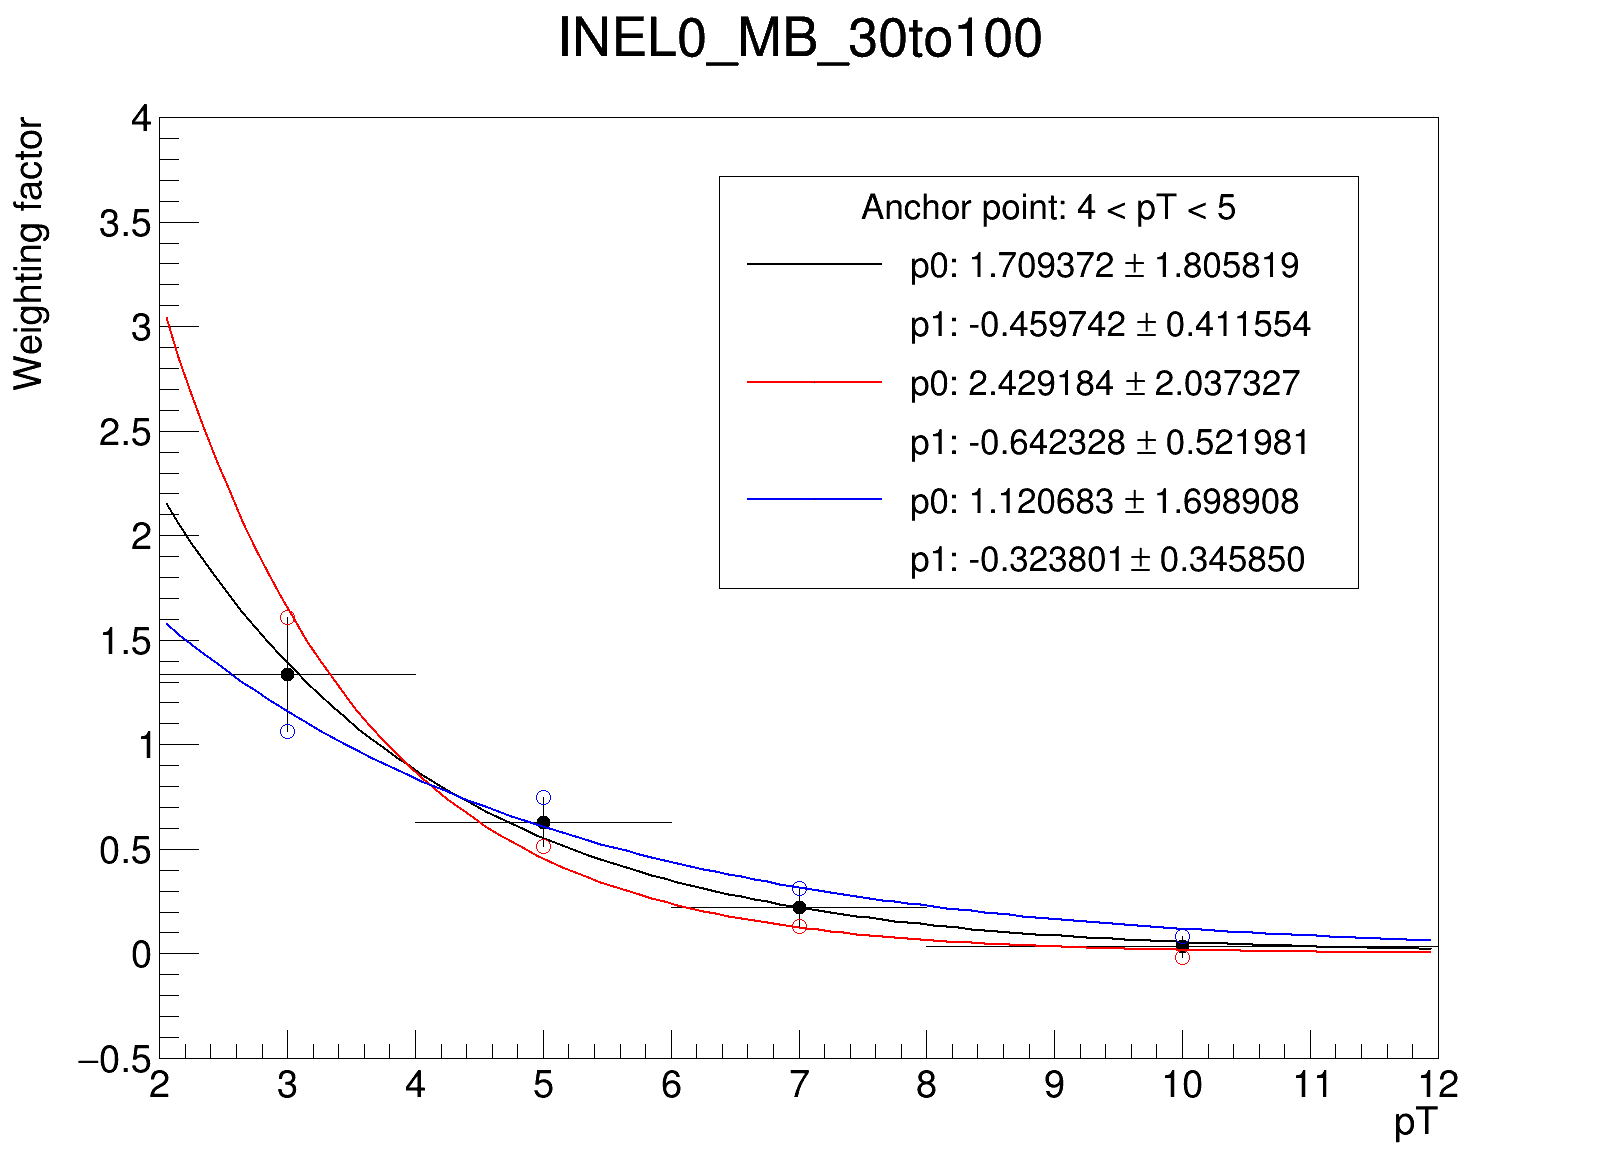
\includegraphics[width=0.45\textwidth]{plots/s2_pTW2to12_INEL0_MB_30to100.png}
    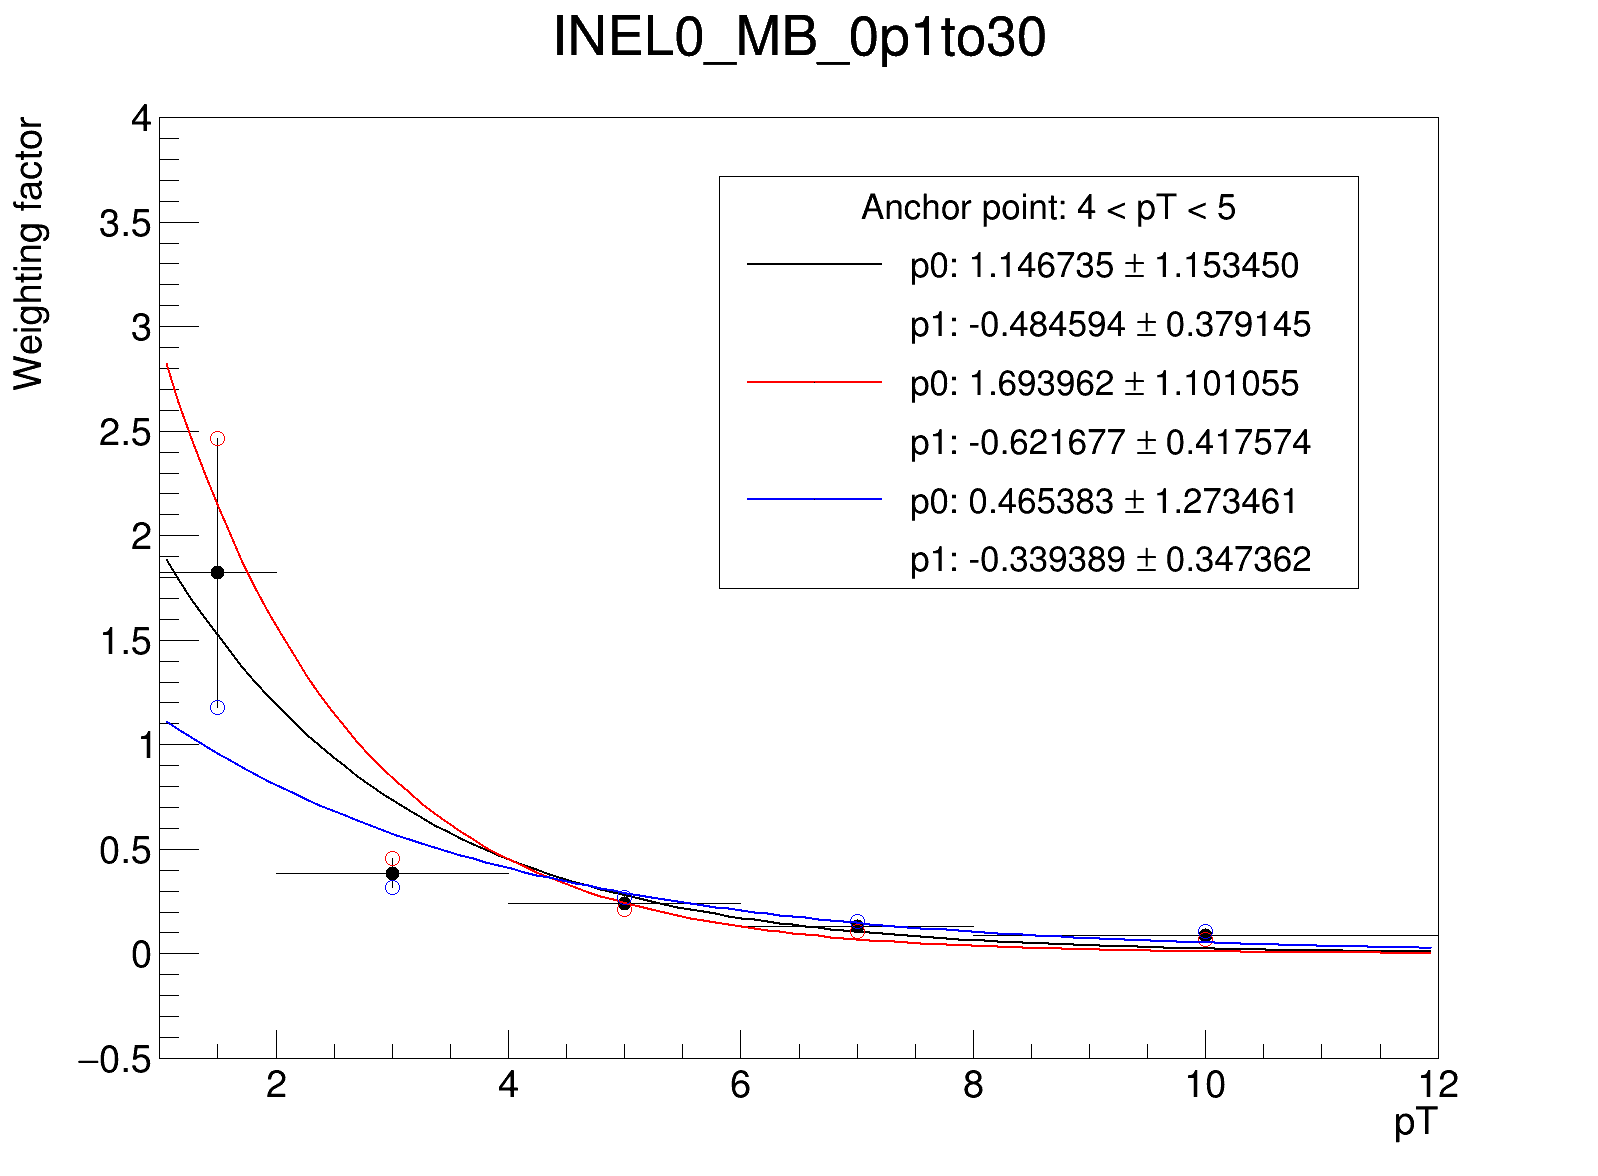
\includegraphics[width=0.45\textwidth]{plots/s2_pTW1to12_INEL0_MB_0p1to30.png}
    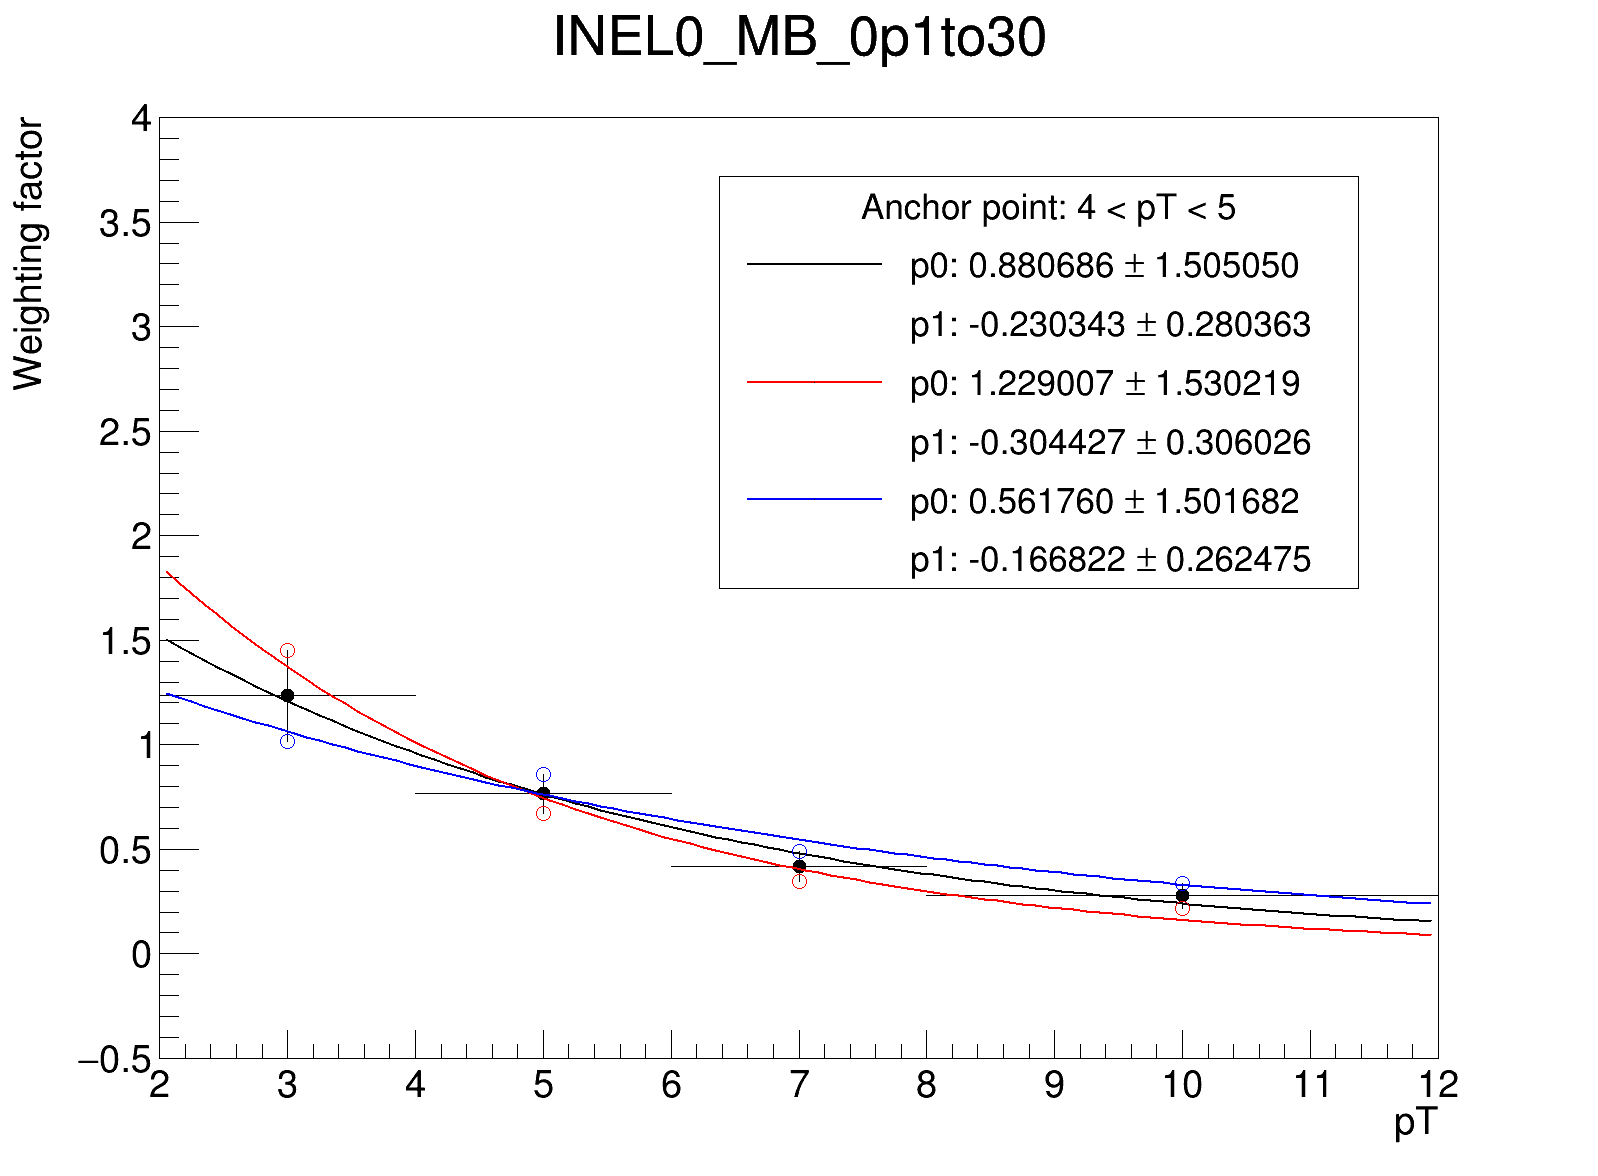
\includegraphics[width=0.45\textwidth]{plots/s2_pTW2to12_INEL0_MB_0p1to30.png}
    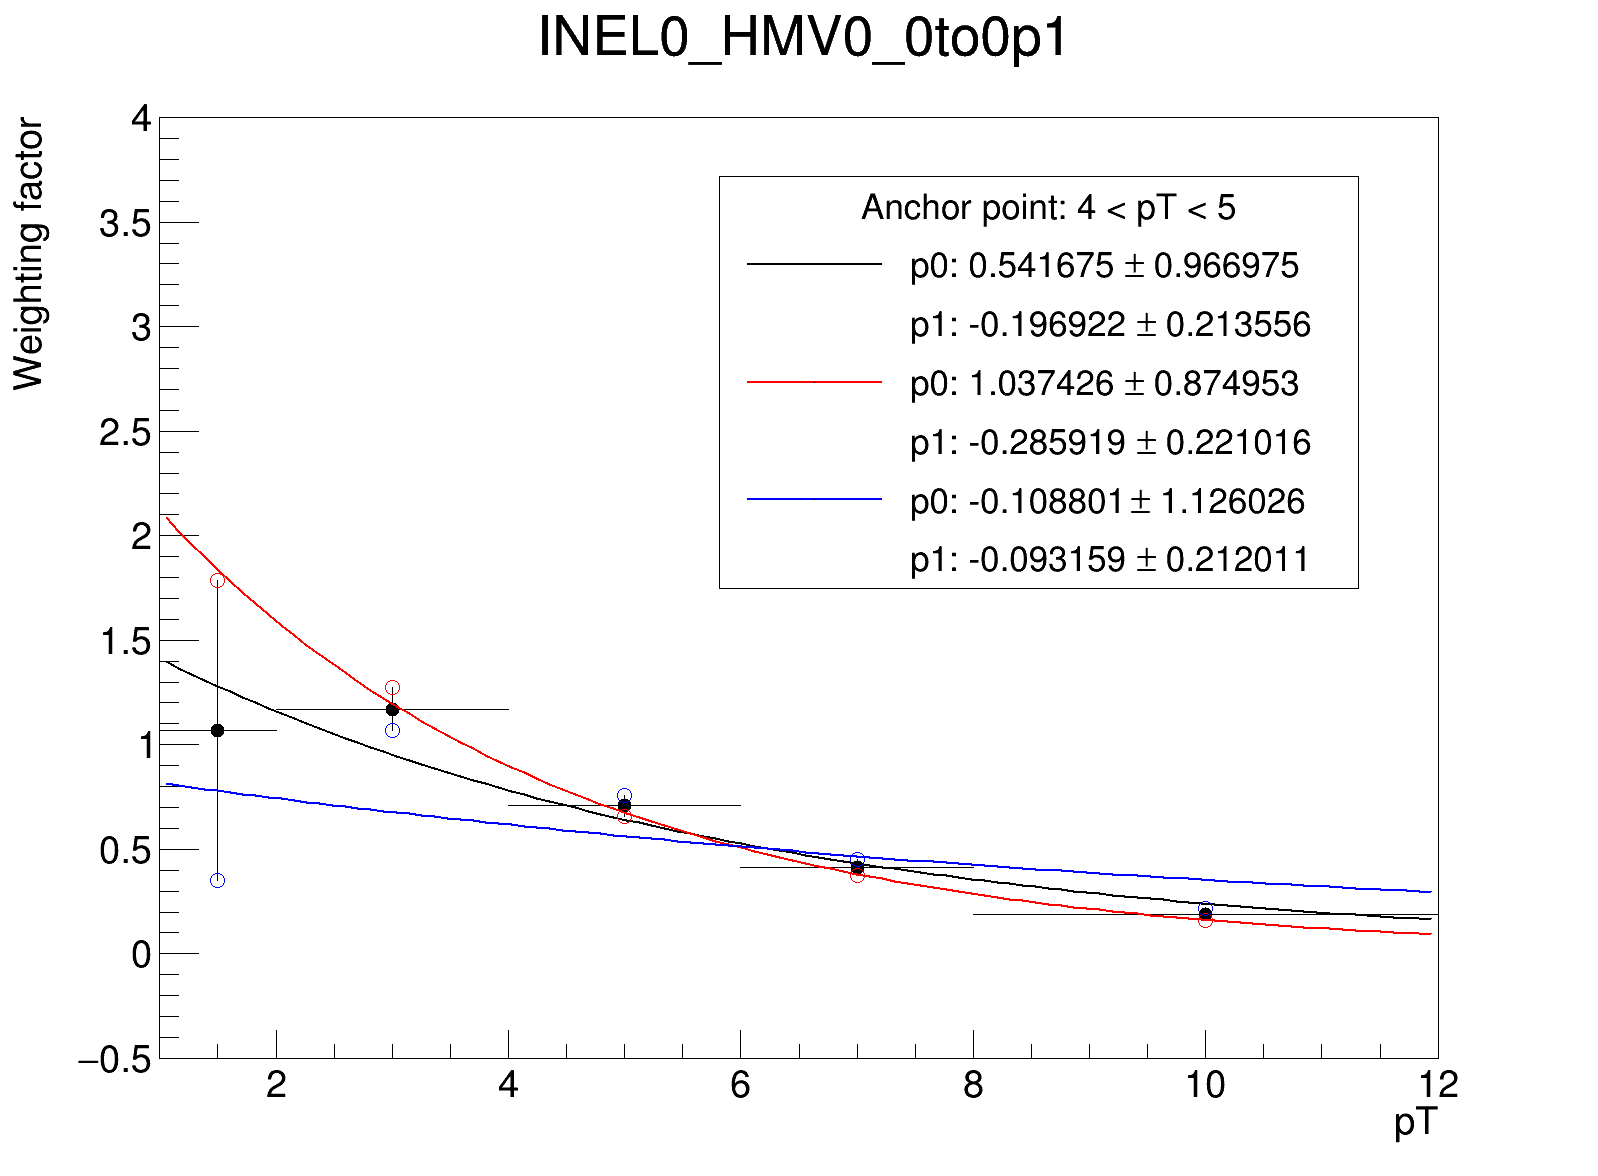
\includegraphics[width=0.45\textwidth]{plots/s2_pTW1to12_INEL0_HMV0_0to0p1.png}
    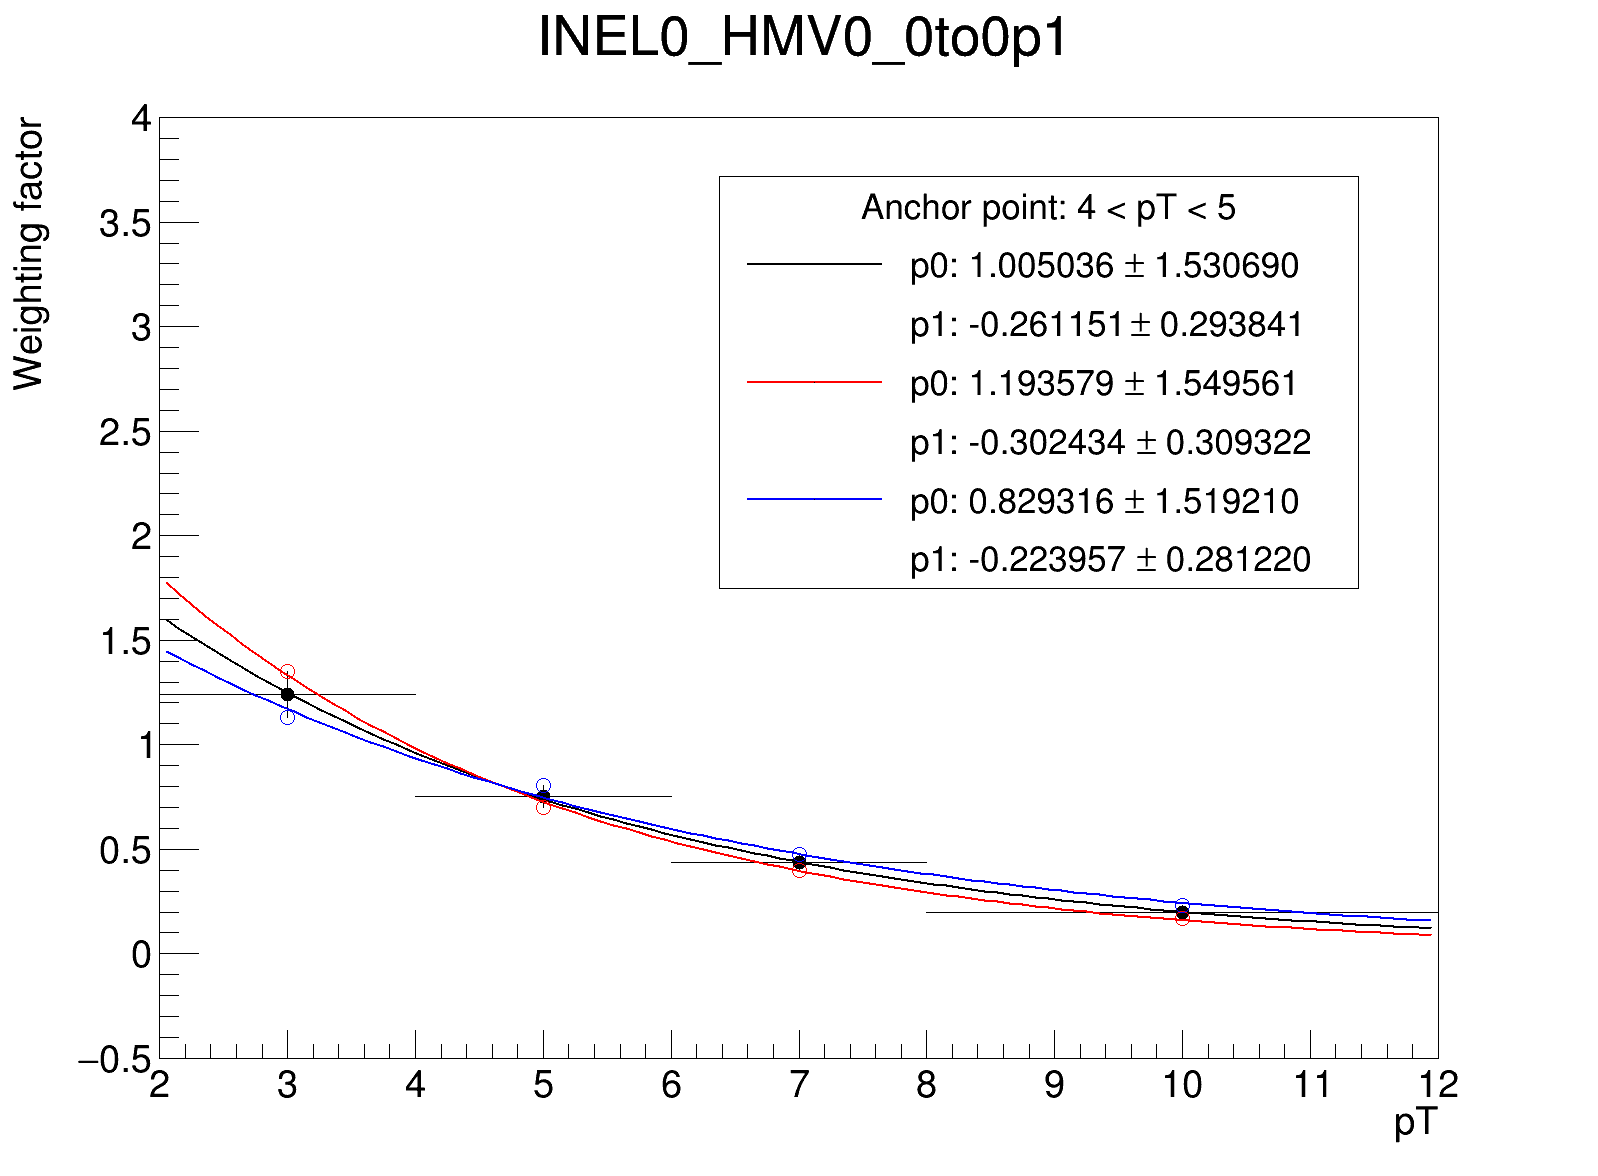
\includegraphics[width=0.45\textwidth]{plots/s2_pTW2to12_INEL0_HMV0_0to0p1.png}
    \caption{Study on weighting factor for each configuration: the points on each pad indicate data/MC ratio of normalized invariant cross-section (no weighting factors applied on MC at this stage) and the colored lines indicate weighting factors by fit (black: central, red/blue: variations with respect to the anchor point 4 $<$ \pt $<$ 5). Left column shows the factor obtained by including \pt range of 1 $<$ \pt $<$ 2 whie Right columne is not.}
    \label{fig:s2_pTW}
\end{figure}

\clearpage
%-----------------------------------------------
\subsubsection{Pair mass cut dependence on low \pt region}
\red{TBU}

\subsubsection{Multiplicity dependence of \Xib over-subtraction}
\red{TBU} \clearpage
\section{Result}\label{sec:result}

%--------------------------------------------------------

\subsection{Systematic errors}
\red{TBU} Error: $|\text{condition\_vary - default}|$ / default * 100 (convert to \%)

\vspace{\columnsep}
\begin{table}[h]
    \centering
    \small
    \begin{tabular}{l|l|l}
    \hline\hline
    Item & Default & Tested \\\hline
    %
    \multicolumn{3}{l}{Online event selection} \\\hline
    ITS-TPC matching & \red{Quote \cite{ana990_Xic0}} & \red{TBU} \\
    Electron track selection & stand (table \ref{tab:eReco}) & vloose, loose, tight, and vtight \\
    \Xis daughter track selection & stand (table \ref{tab:XiReco}) & vloose, loose, tight, and vtight \\
    Rapidity ($|$\textit{y}$|$) interval sensitivity & 0.5 & 0.8 \\\hline
    %
    \multicolumn{3}{l}{Offline event selection} \\\hline
    Electron pID & stand (table \ref{tab:ePID}) & vloose, loose, tight, and vtight \\
    \Xis pID by topology & stand (table \ref{tab:XiPID}) & vloose, loose, tight, and vtight \\
    e-\Xim pair selection: mass & 2.5 (table \ref{tab:eXiPair}) & 2.3 and 2.7 \\
    e-\Xim pair selection: opening angle & 90 (table \ref{tab:eXiPair}) & 70 \\\hline
    %
    \multicolumn{3}{l}{Offline analysis} \\\hline
    Unfolding: method & Bayesian & SVD \\
    Unfolding: \# of iterations & 3 & 2, 4, 5, 6, and 7 \\
    Unfolding: \pt range & [1, 2, 4, 6, 8, 12, 14] & [1, 2, 4, 6, 8, 12] and \\
    && [0, 1, 2, 4, 6, 8, 12, 24] \\
    \Xib over-subtraction correction & \red{Disabled} & \red{TBU} \\
    Feed-down subtraction            & \red{Disabled} & \red{TBU} \\
    Generated \pt shape & & \\
    %
    \hline\hline
    \end{tabular}
    \caption{Table of items for systematic error and conditions tested}
    \label{tab:systItems}
\end{table}

\begin{figure}
    \centering
    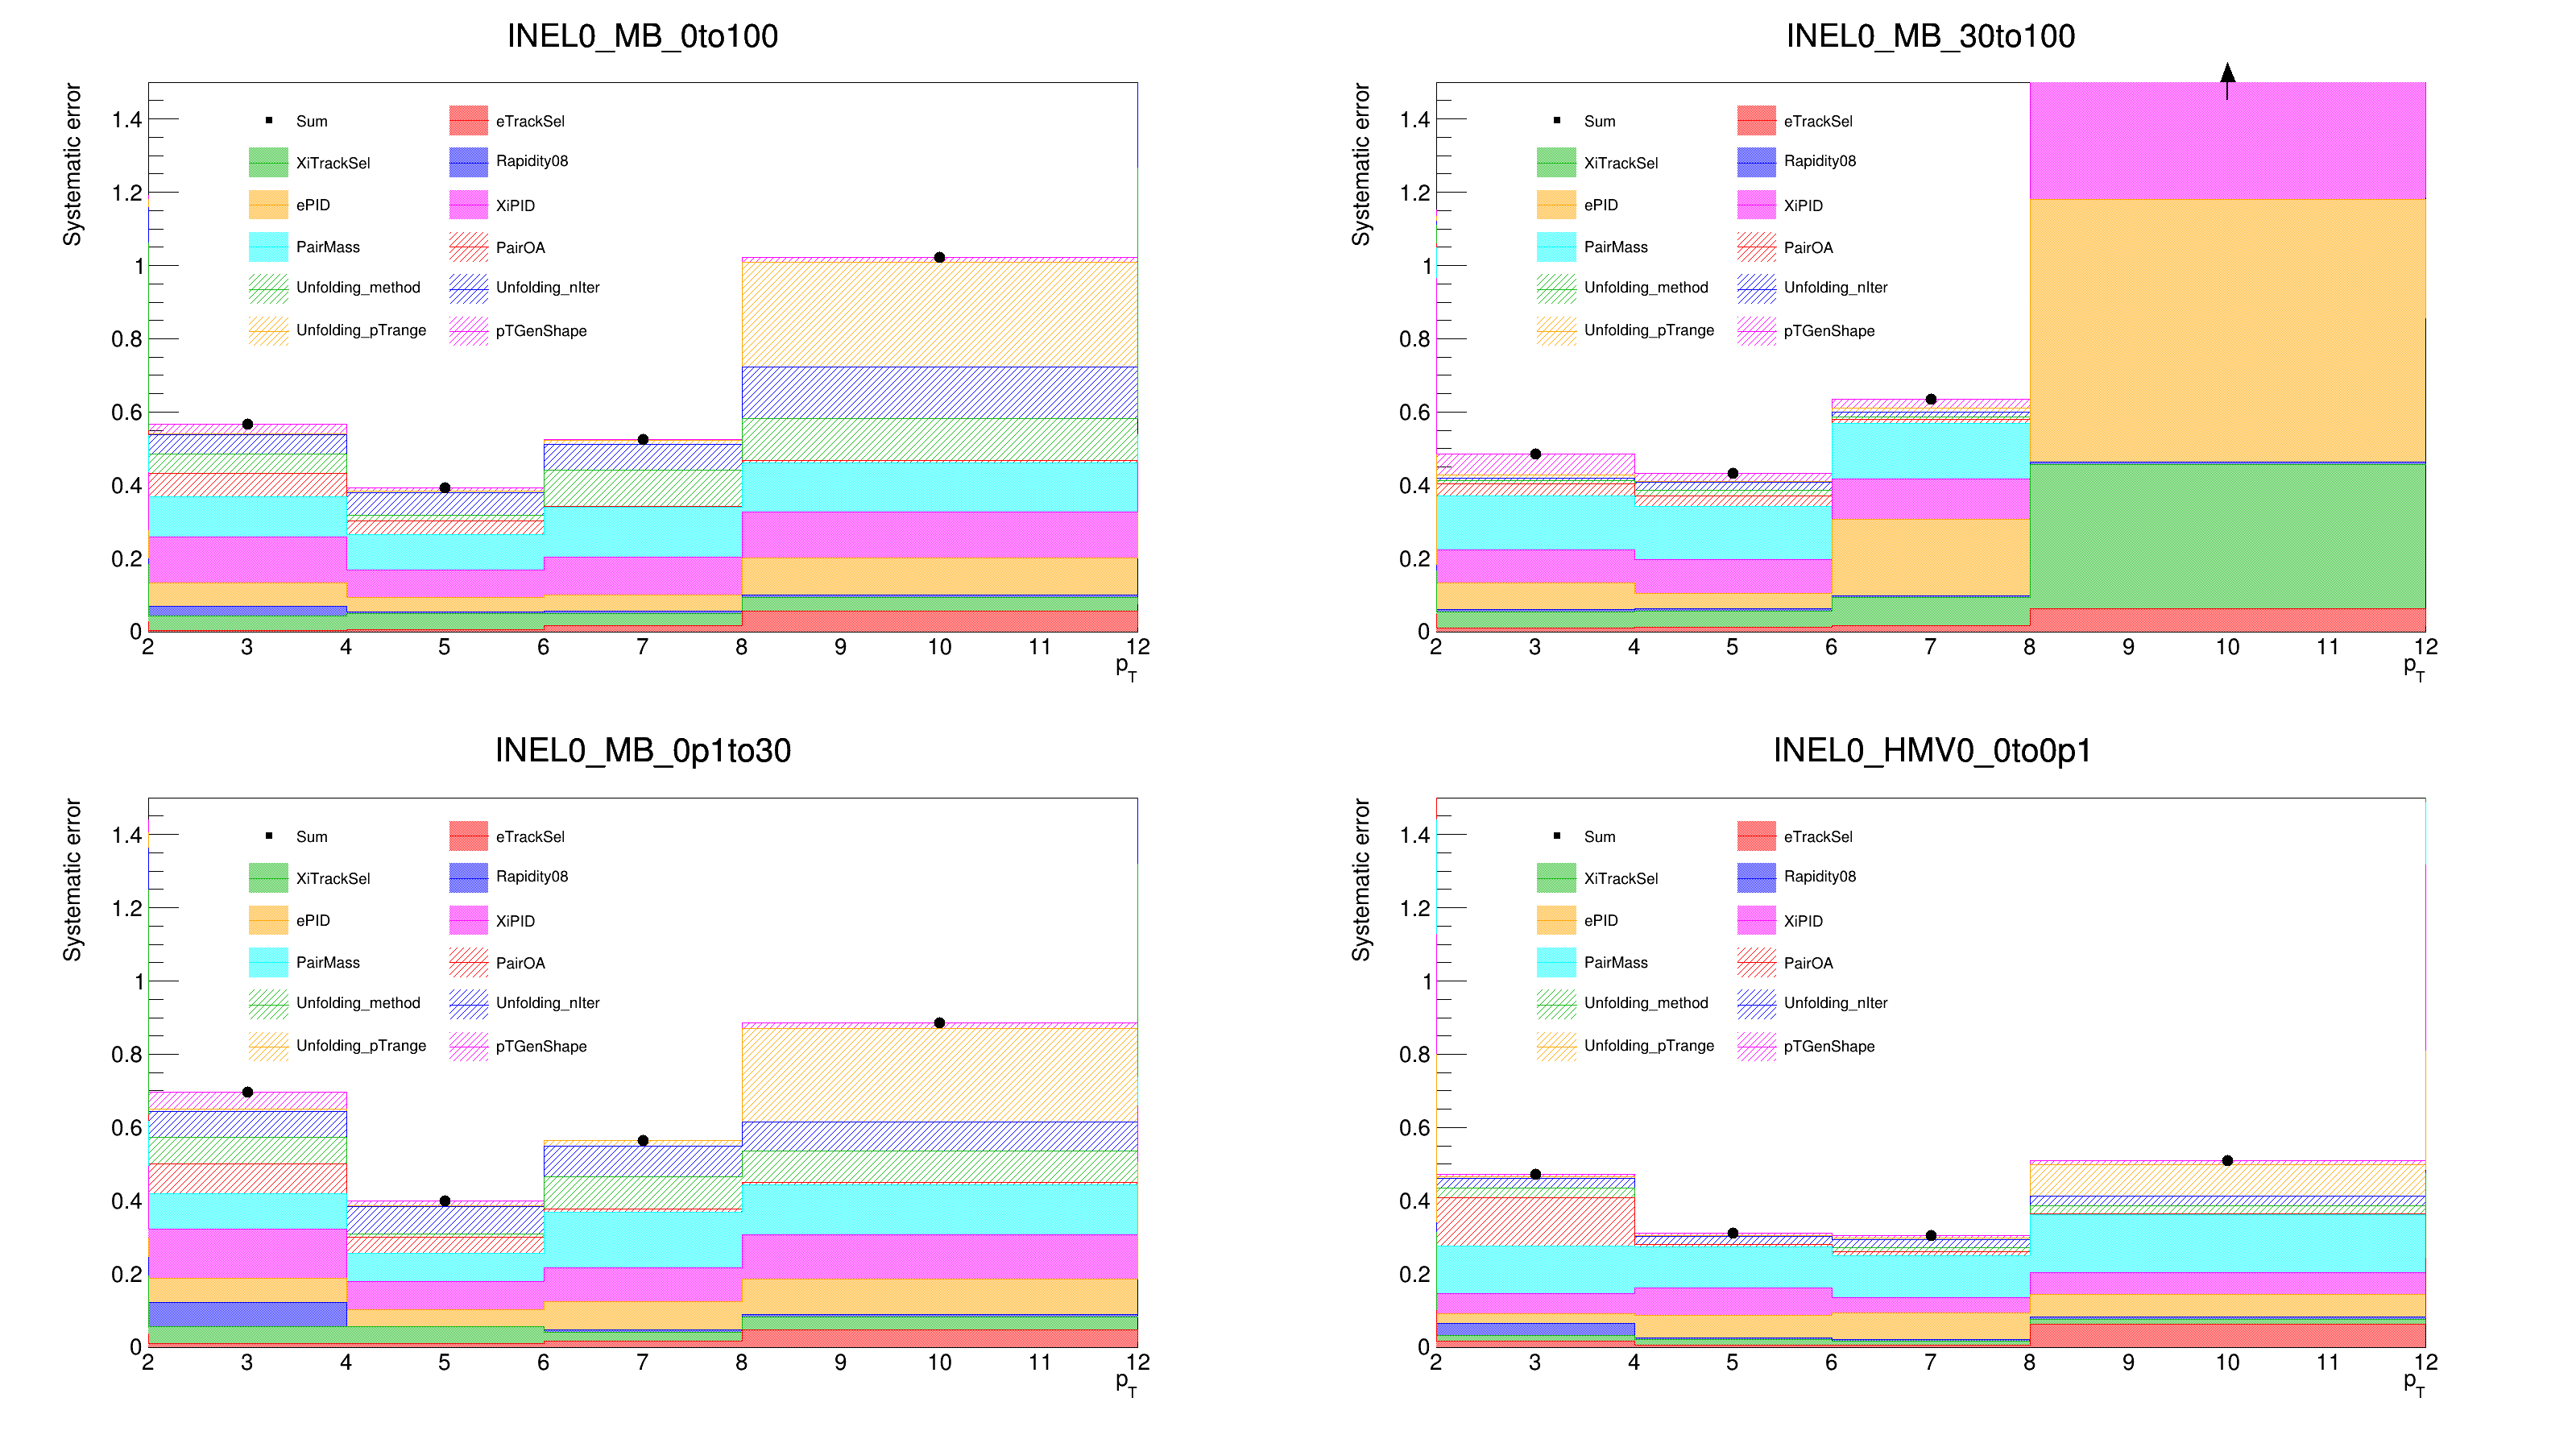
\includegraphics[width=0.95\textwidth]{plots/s3_SystErr_2to12.png}
    \caption{A}
    \label{fig:s3_systErr}
\end{figure}

\clearpage
\begin{table}[t]
    \centering
    \small
    \begin{tabular}{l|rrrr}
    \hline\hline
    \multicolumn{5}{c}{\normalsize \blue{MB + [0, 100]}} \\\hline
    \multirow{2}{*}{Item \red{(* error unit: \%)}} & \multicolumn{4}{c}{\pt (\GeVc)} \\\cline{2-5}
    & 2-4 & 4-6 & 6-8 & 8-12 \\\hline
    %
    \multicolumn{5}{l}{Online event selection} \\\hline
    ITS-TPC matching & \red{2.5} & \red{2.5} & \red{2.5} & \red{2.5} \\
    Electron track selection                   &  0.4 &  0.7 &  1.7 &  5.6 \\
    \Xis daughter track selection              &  3.9 &  4.4 &  3.3 &  3.8 \\
    Rapidity (\textit{y}) interval sensitivity &  2.7 &  0.5 &  0.6 &  0.7 \\
    \hline
    %
    \multicolumn{5}{l}{Offline event selection} \\\hline
    Electron pID                         &  6.4 &  3.8 &  4.5 & 10.0 \\
    \Xis pID by topology                 & 12.6 &  7.6 & 10.3 & 12.6 \\
    e-\Xim pair selection: mass          & 10.8 &  9.6 & 13.6 & 13.3 \\
    e-\Xim pair selection: opening angle &  6.4 &  3.7 &  0.3 &  0.7 \\
    \hline
    %
    \multicolumn{5}{l}{Offline analysis} \\\hline
    Unfolding: method                &  5.3 &  1.6 &  9.9 & 11.4 \\
    Unfolding: \# of iterations      &  5.4 &  6.3 &  7.1 & 14.0 \\
    Unfolding: \pt range             &  0.1 &  0.3 &  1.1 & 28.8 \\
    \Xib over-subtraction correction & \multicolumn{4}{c}{\red{TBU}} \\
    Feed-down subtraction            & \multicolumn{4}{c}{\red{TBU}} \\
    Generated \pt shape              &  2.7 &  0.9 &  0.1 &  1.2 \\
    \hline
    %
    Total & 21.2 & 15.7 & 21.9 & 40.6 \\
    \hline\hline
    \end{tabular}
    \caption{Table of systematic errors for configuration MB + [0, 100]}
    \label{tab:systMB_0to100}
\end{table}

\begin{table}[b]
    \centering
    \small
    \begin{tabular}{l|rrrr}
    \hline\hline
    \multicolumn{5}{c}{\normalsize \blue{MB + [30, 100]}} \\\hline
    \multirow{2}{*}{Item \red{(* error unit: \%)}} & \multicolumn{4}{c}{\pt (\GeVc)} \\\cline{2-5}
    & 2-4 & 4-6 & 6-8 & 8-12 \\\hline
    %
    \multicolumn{5}{l}{Online event selection} \\\hline
    ITS-TPC matching & \red{2.5} & \red{2.5} & \red{2.5} & \red{2.5} \\
    Electron track selection                   &  1.1 &  1.3 &  1.7 &  6.4 \\
    \Xis daughter track selection              &  4.2 &  4.4 &  7.6 & 39.3 \\
    Rapidity (\textit{y}) interval sensitivity &  0.7 &  0.8 &  0.5 &  0.7 \\
    \hline
    %
    \multicolumn{5}{l}{Offline event selection} \\\hline
    Electron pID                         &  7.3 &  4.0 & 21.0 & 71.7 \\
    \Xis pID by topology                 &  9.2 &  9.4 & 10.9 & 79.1 \\
    e-\Xim pair selection: mass          & 14.5 & 14.3 & 15.1 & 22.7 \\
    e-\Xim pair selection: opening angle &  3.3 &  3.0 &  1.1 &  0.9 \\
    \hline
    %
    \multicolumn{5}{l}{Offline analysis} \\\hline
    Unfolding: method                &  0.9 &  1.4 &  0.8 & 89.3 \\
    Unfolding: \# of iterations      &  0.8 &  2.3 &  1.2 & 60.2 \\
    Unfolding: \pt range             &  0.8 &  0.2 &  1.1 & 32.5 \\
    \Xib over-subtraction correction & \multicolumn{4}{c}{\red{TBU}} \\
    Feed-down subtraction            & \multicolumn{4}{c}{\red{TBU}} \\
    Generated \pt shape              &  5.7 &  2.1 &  2.3 &  0.8 \\
    \hline
    %
    Total & 20.5 & 18.9 & 29.4 & 161.8 \\
    \hline\hline
    \end{tabular}
    \caption{Table of systematic errors for configuration MB + [30, 100]}
    \label{tab:systMB_30to100}
\end{table}

\clearpage
\begin{table}[t]
    \centering
    \small
    \begin{tabular}{l|rrrrr}
    \hline\hline
    \multicolumn{5}{c}{\normalsize \blue{MB + [0.1, 30]}} \\\hline
    \multirow{2}{*}{Item \red{(* error unit: \%)}} & \multicolumn{4}{c}{\pt (\GeVc)} \\\cline{2-5}
    & 2-4 & 4-6 & 6-8 & 8-12 \\\hline
    %
    \multicolumn{5}{l}{Online event selection} \\\hline
    ITS-TPC matching & \red{2.5} & \red{2.5} & \red{2.5} & \red{2.5} \\
    Electron track selection                   &  1.1 &  1.0 &  1.8 &  4.7 \\
    \Xis daughter track selection              &  4.5 &  4.6 &  2.4 &  3.5 \\
    Rapidity (\textit{y}) interval sensitivity &  6.6 &  0.0 &  0.6 &  0.7 \\
    \hline
    %
    \multicolumn{5}{l}{Offline event selection} \\\hline
    Electron pID                         &  6.6 &  4.5 &  7.6 &  9.8 \\
    \Xis pID by topology                 & 13.6 &  7.7 &  9.3 & 12.1 \\
    e-\Xim pair selection: mass          &  9.5 &  7.9 & 15.2 & 13.5 \\
    e-\Xim pair selection: opening angle &  8.3 &  4.3 &  0.8 &  0.8 \\
    \hline
    %
    \multicolumn{5}{l}{Offline analysis} \\\hline
    Unfolding: method                &  7.3 &  0.8 &  8.9 &  8.6 \\
    Unfolding: \# of iterations      &  7.1 &  7.5 &  8.3 &  7.9 \\
    Unfolding: \pt range             &  0.5 &  0.3 &  1.4 & 25.3 \\
    \Xib over-subtraction correction & \multicolumn{4}{c}{\red{TBU}} \\
    Feed-down subtraction            & \multicolumn{4}{c}{\red{TBU}} \\
    Generated \pt shape              &  4.8 &  1.1 &  0.1 &  1.6 \\
    \hline
    %
    Total & 24.1 & 15.7 & 23.3 & 35.3 \\
    \hline\hline
    \end{tabular}
    \caption{Table of systematic errors for configuration MB + [0.1, 30]}
    \label{tab:systMB_0p1to30}
\end{table}

\begin{table}[b]
    \centering
    \small
    \begin{tabular}{l|rrrrr}
    \hline\hline
    \multicolumn{5}{c}{\normalsize \blue{HMV0 + [0, 0.1]}} \\\hline
    \multirow{2}{*}{Item \red{(* error unit: \%)}} & \multicolumn{4}{c}{\pt (\GeVc)} \\\cline{2-5}
    & 2-4 & 4-6 & 6-8 & 8-12 \\\hline
    %
    \multicolumn{5}{l}{Online event selection} \\\hline
    ITS-TPC matching & \red{2.5} & \red{2.5} & \red{2.5} & \red{2.5} \\
    Electron track selection                   &  1.7 &  0.6 &  0.6 &  6.4 \\
    \Xis daughter track selection              &  1.5 &  1.6 &  1.1 &  1.3 \\
    Rapidity (\textit{y}) interval sensitivity &  3.4 &  0.3 &  0.5 &  0.7 \\
    \hline
    %
    \multicolumn{5}{l}{Offline event selection} \\\hline
    Electron pID                         &  2.6 &  6.2 &  7.2 &  6.1 \\
    \Xis pID by topology                 &  5.5 &  7.4 &  4.1 &  5.9 \\
    e-\Xim pair selection: mass          & 12.9 & 11.3 & 11.6 & 15.8 \\
    e-\Xim pair selection: opening angle & 13.3 &  0.6 &  0.9 &  0.3 \\
    \hline
    %
    \multicolumn{5}{l}{Offline analysis} \\\hline
    Unfolding: method                &  2.5 &  0.0 &  1.1 &  2.2 \\
    Unfolding: \# of iterations      &  2.7 &  2.3 &  2.2 &  2.7 \\
    Unfolding: \pt range             &  0.4 &  0.1 &  0.6 &  8.5 \\
    \Xib over-subtraction correction & \multicolumn{4}{c}{\red{TBU}} \\
    Feed-down subtraction            & \multicolumn{4}{c}{\red{TBU}} \\
    Generated \pt shape              &  0.8 &  0.6 &  0.5 &  1.1 \\
    \hline
    %
    Total & 20.4 & 15.4 & 14.8 & 21.4 \\
    \hline\hline
    \end{tabular}
    \caption{Table of systematic errors for configuration HMV0 + [0, 0.1]}
    \label{tab:systHMV0_0to0p1}
\end{table}

\iffalse
\begin{table}[h]
    \centering
    \small
    \begin{tabular}{l|r|r|r|r|r|r}
    \hline\hline
    \multicolumn{7}{c}{\normalsize \blue{CONF}} \\\hline
    \multirow{2}{*}{Item} & \multicolumn{6}{c}{\pt (\GeVc)} \\\cline{2-7}
    & 1-2 & 2-4 & 4-6 & 6-8 & 8-12 & 12-24 \\\hline
    %
    \multicolumn{7}{l}{Online event selection} \\\hline
    ITS-TPC matching                           & & & \red{2.5} & & & \\
    Electron track selection                   & & & & & & \\
    \Xis daughter track selection              & & & & & & \\
    Rapidity (\textit{y}) interval sensitivity & & & & & & \\
    \hline
    %
    \multicolumn{7}{l}{Offline event selection} \\\hline
    Electron pID                         & & & & & & \\
    \Xis pID by topology                 & & & & & & \\
    e-\Xim pair selection: mass          & & & & & & \\
    e-\Xim pair selection: opening angle & & & & & & \\\hline
    %
    \multicolumn{7}{l}{Offline analysis} \\\hline
    Unfolding: method                & & & & & & \\
    Unfolding: \# of iterations      & & & & & & \\
    Unfolding: \pt range and binning & & & & & & \\
    \Xib over-subtraction correction & & & & & & \\
    Feed-down subtraction            & & & & & & \\
    Generated \pt shape              & & & & & & \\\hline
    %
    Total & & & & & & \\
    %
    \hline\hline
    \end{tabular}
    \caption{Table of systematic errors]}
    \label{tab:syst}
\end{table}
\fi

\clearpage
%--------------------------------------------------------

\subsection{\Xic yields and \Xic/\Dzero ratio}
\red{TBU}

\begin{figure}[h]
    \centering
    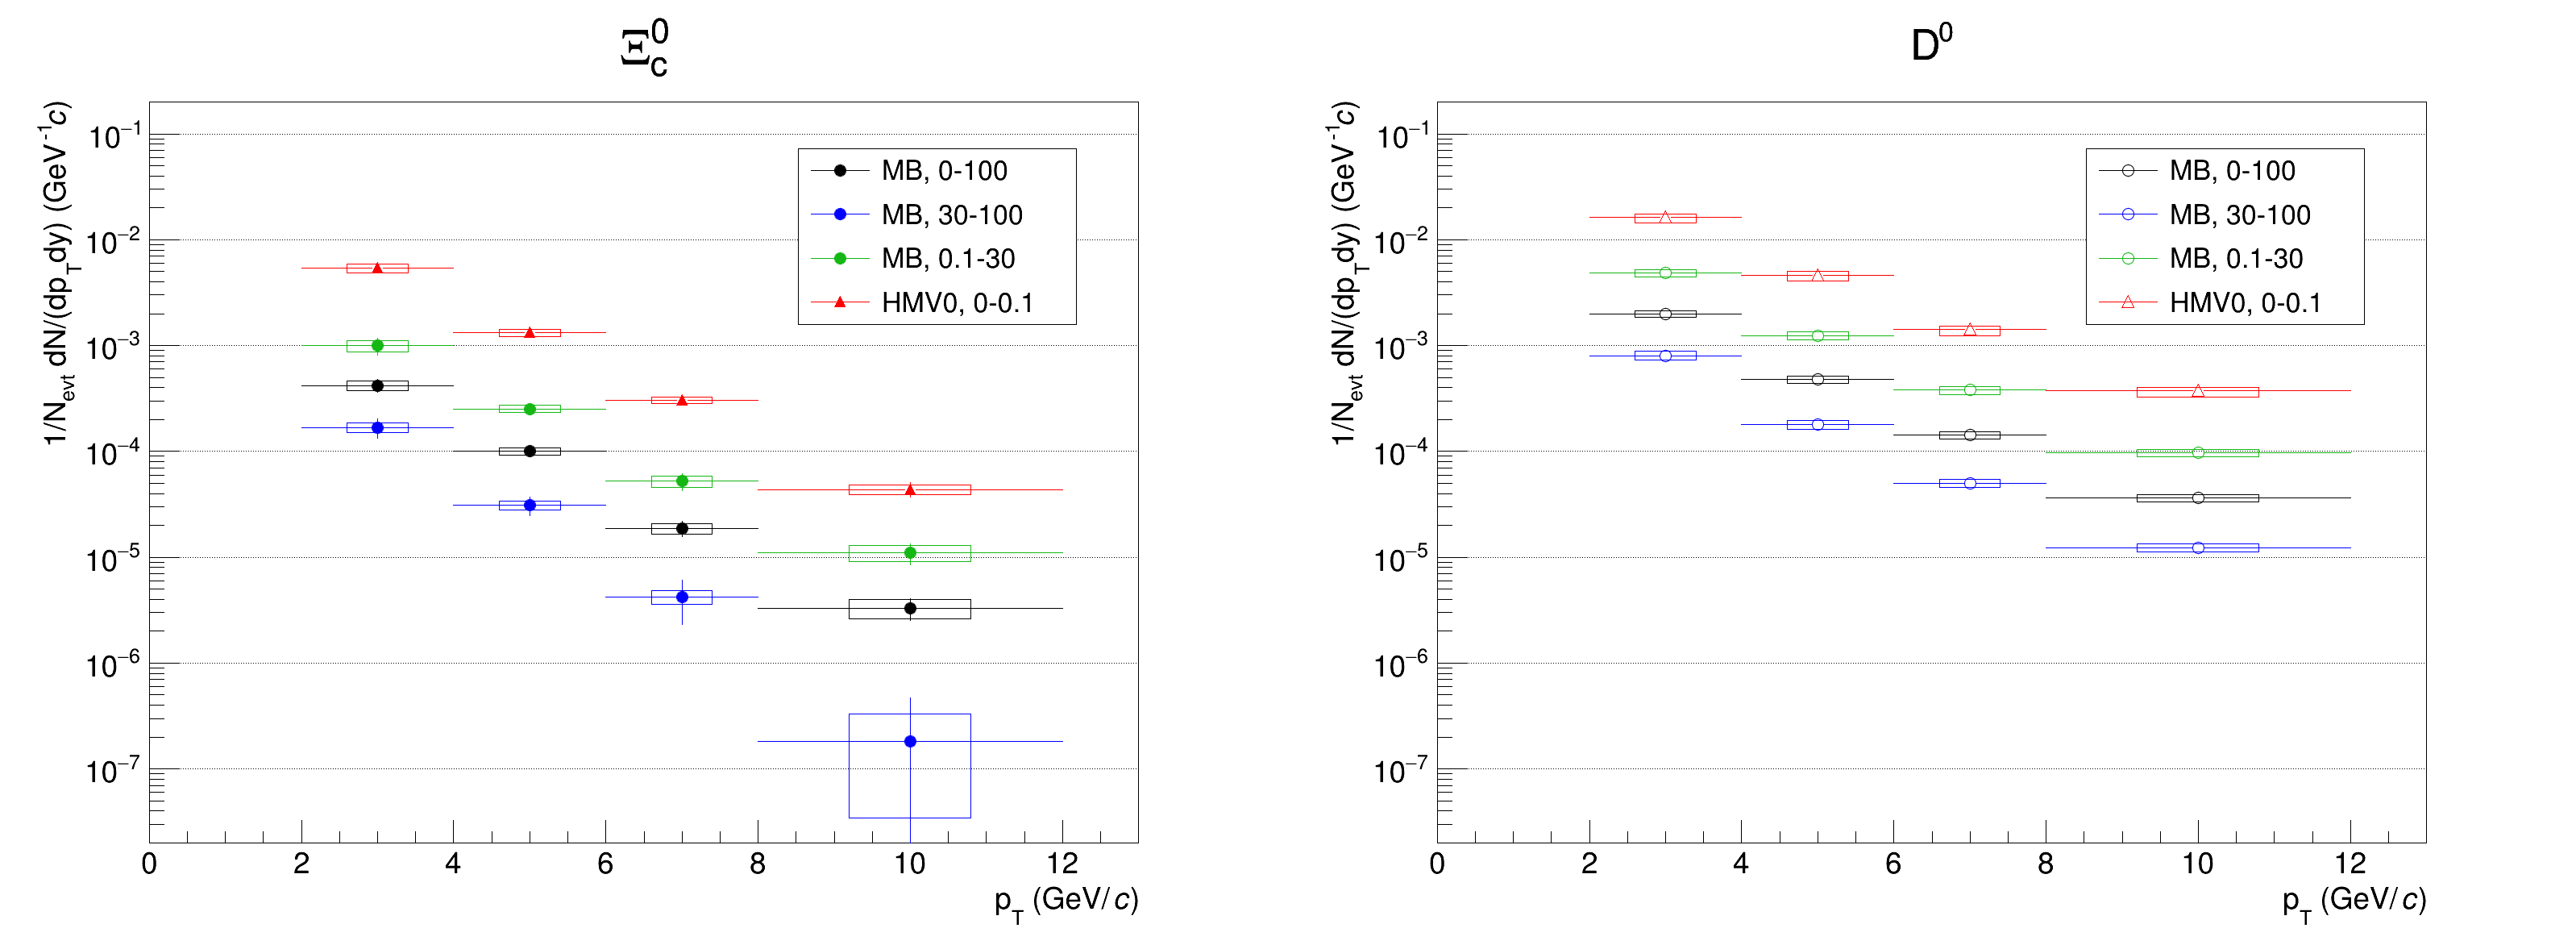
\includegraphics[width=0.95\textwidth]{plots/s3_Yield_INEL0.png}
    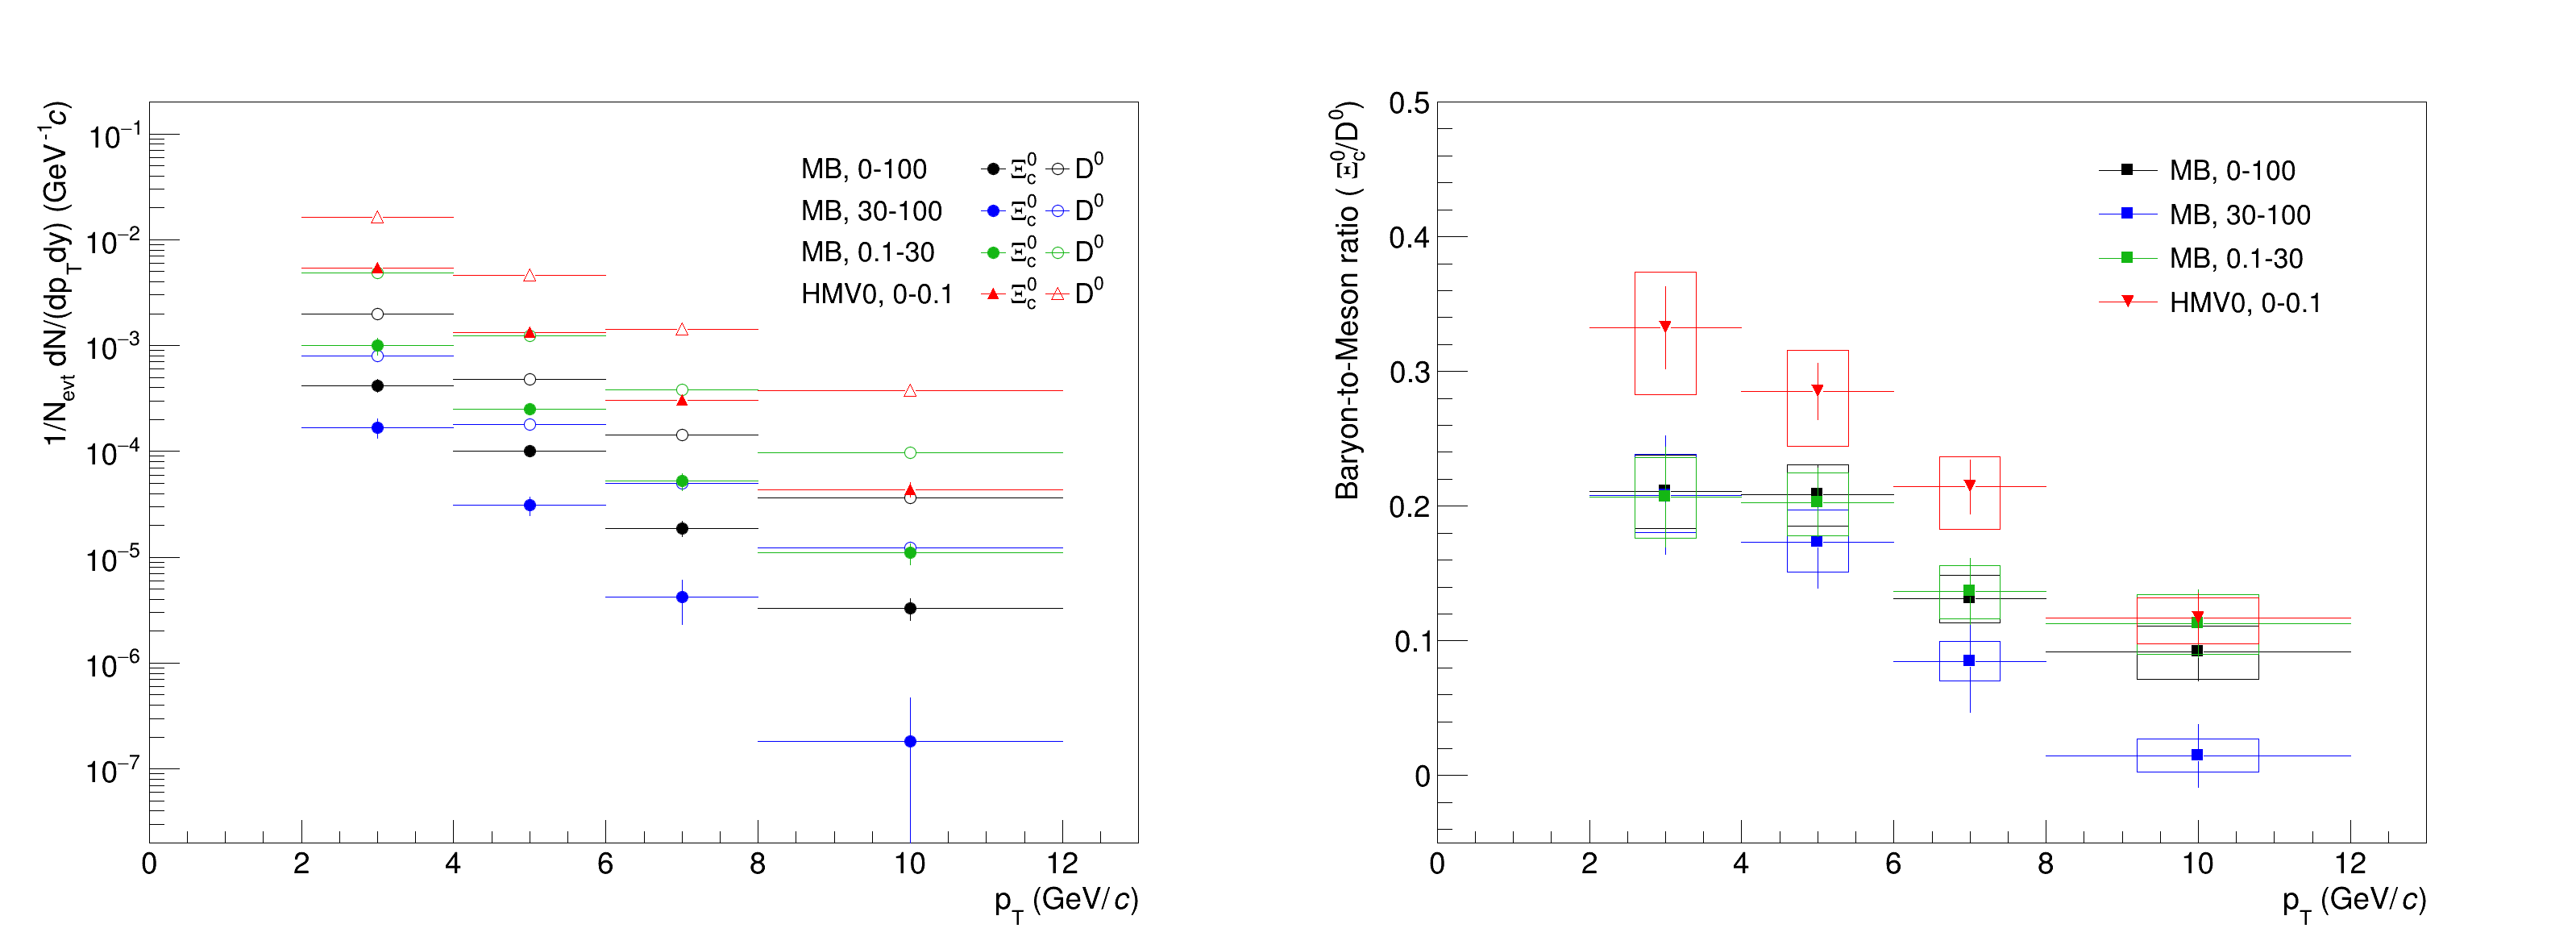
\includegraphics[width=0.95\textwidth]{plots/s3_Ratio_INEL0.png}
    \caption{Normalized invariant cross-section of \Xic (top left) and \Dzero (top right) \cite{ana993_D0}.
    The bottom left shows the cross-sections together and The bottom right shows the baryon-to-meson ratio calculated by \Xic/\Dzero.}
    \label{fig:s3_results}
\end{figure}

 \clearpage
\begin{appendix}

%--------------------------------------------

\section{Full list of runs}\label{sec:appA}
\red{TBU}

\vspace{\columnsep}
\begin{itemize}
    \small
    \item[] \blue{LHC16: d, e, g, h, j, o, p, k, and l}
    \footnotesize
    \item[-] LHC16d\_pass2:\\[1pt]
     252375, 252374, 252371, 252370, 252368, 252336, 252332, 252330, 252326, 252325,\\
     252322, 252319, 252317, 252310, 252271, 252248, 252235
    \item[-] LHC16e\_pass2:\\[1pt]
     253591, 253589, 253563, 253530, 253529, 253517, 253488, 253482, 253481, 253478,\\
     253437, 252867, 252858
    \item[-] LHC16g\_pass2:\\[1pt]
     254332, 254331, 254330, 254304, 254303, 254302, 254293, 254205, 254204, 254199,\\
     254193, 254178, 254175, 254174, 254149, 254147, 254128
    \item[-] LHC16h\_pass2\_positiveMagField:\\[1pt]
     255469, 255467, 255466, 255465, 255463, 255447, 255442, 255440, 255421, 255420,\\
     255419, 255418, 255415, 255407, 255402, 255398, 255352, 255351, 255350, 255283,\\
     255280, 255276, 255275, 255256, 255255, 255253, 255252, 255251, 255249, 255248,\\
     255247, 255242, 255240, 255182, 255181, 255180, 255177, 255176, 255174, 255173,\\
     255171, 255167, 255162, 255159, 255154, 255111, 255091, 255086, 255085, 255082,\\
     255079, 254984, 254983, 254654, 254653, 254652, 254651, 254649, 254648, 254646,\\
     254644, 254640, 254632, 254630, 254629, 254621, 254606, 254604
    \item[-] LHC16j\_pass2:\\[1pt]
     256418, 256417, 256415, 256373, 256372, 256371, 256368, 256366, 256365, 256364,\\
     256363, 256362, 256361, 256356, 256311, 256309, 256307, 256302, 256299, 256297,\\
     256295, 256292, 256290, 256289, 256287, 256284, 256283, 256282, 256281, 256231,\\
     256228, 256227, 256225, 256223, 256219
    \item[-] LHC16o\_pass2\_hadronPID:\\[1pt]
     264035, 264033, 263985, 263984, 263981, 263978, 263977, 263923, 263920, 263917,\\
     263916, 263905, 263866, 263863, 263810, 263803, 263793, 263792, 263790, 263787,\\
     263786, 263785, 263784, 263744, 263743, 263741, 263739, 263738, 263737, 263691,\\
     263690, 263682, 263663, 263662, 263657, 263654, 263652, 263647, 263529, 263497,\\
     263496, 263490, 263487, 263332, 263331, 262858, 262855, 262853, 262849, 262847,\\
     262844, 262842, 262841, 262778, 262777, 262776, 262768, 262760, 262727, 262725,\\
     262723, 262719, 262717, 262713, 262708, 262706, 262705, 262428, 262426, 262425,\\
     262424
    \item[-] LHC16o\_pass2\_incompleteTPC:\\[1pt]
     263979, 262635, 262632, 262628, 262624, 262594, 262593, 262583, 262578, 262574,\\
     262572, 262571, 262570, 262569, 262568, 262567, 262563, 262537, 262533, 262532,\\
     262528, 262492, 262490, 262489, 262487, 262451, 262450, 262430, 263861
    \item[-] LHC16p\_pass2:\\[1pt]
     264347, 264346, 264345, 264341, 264336, 264312, 264306, 264305, 264281, 264279,\\
     264277, 264273, 264267, 264266, 264265, 264264, 264262, 264261, 264260, 264259,\\
     264238, 264235, 264233, 264232, 264198, 264197, 264194, 264190, 264188, 264168,\\
     264164, 264139, 264138, 264137, 264129, 264110, 264109, 264086, 264085, 264082,\\
     264078, 264076
    \item[-] LHC16k\_pass2\_hadronPID:\\[1pt]
     258537, 258499, 258477, 258456, 258454, 258452, 258426, 258393, 258391, 258387,\\
     258359, 258336, 258332, 258307, 258306, 258303, 258302, 258301, 258299, 258278,\\
     258274, 258273, 258271, 258270, 258258, 258257, 258256, 258204, 258203, 258202,\\
     258198, 258197, 258178, 258117, 258114, 258113, 258109, 258108, 258107, 258063,\\
     258062, 258060, 258059, 258053, 258049, 258045, 258042, 258041, 258039, 258019,\\
     258017, 258014, 258012, 258008, 258003, 257992, 257989, 257986, 257979, 257963,\\
     257960, 257957, 257939, 257937, 257936, 257855, 257853, 257851, 257850, 257804,\\
     257803, 257800, 257799, 257798, 257797, 257773, 257765, 257757, 257754, 257737,\\
     257735, 257734, 257733, 257727, 257725, 257724, 257697, 257694, 257692, 257691,\\
     257689, 257688, 257687, 257685, 257684, 257682, 257644, 257642, 257636, 257635,\\
     257632, 257630, 257606, 257605, 257604, 257601, 257595, 257594, 257592, 257590,\\
     257588, 257587, 257566, 257562, 257561, 257560, 257541, 257540, 257539, 257537,\\
     257531, 257530, 257492, 257491, 257490, 257488, 257487, 257474, 257468, 257457,\\
     257433, 257364, 257358, 257330, 257322, 257320, 257318, 257260, 257224, 257209,\\
     257206, 257204, 257144, 257141, 257139, 257138, 257137, 257136, 257100, 257095,\\
     257092, 257086, 257084, 257082, 257080, 257077, 257012, 257011, 256944, 256942,\\
     256941
    \item[-] LHC16k\_pass2\_incompleteTPC:\\[1pt]
     258498, 258388, 258280, 257932, 257912, 257901, 257071
    \item[-] LHC16l\_pass2\_hadronPID:\\[1pt]
     259888, 259868, 259867, 259866, 259860, 259842, 259841, 259822, 259789, 259788,\\
     259781, 259756, 259752, 259751, 259750, 259748, 259747, 259477, 259473, 259396,\\
     259395, 259394, 259389, 259388, 259382, 259378, 259342, 259341, 259340, 259339,\\
     259336, 259334, 259307, 259305, 259303, 259302, 259274, 259273, 259272, 259271,\\
     259270, 259269, 259264, 259263, 259261, 259257, 259204, 259164, 259162, 259118,\\
     259117, 259099, 259096, 259091, 259090, 259088, 258964, 258962
    \item[-] LHC16l\_pass2\_incompleteTPC:\\[1pt]
     259381, 259086 
\end{itemize}

\vspace{\columnsep}
\begin{itemize}
    \small
    \item[] \blue{LHC17: c, e, f, h, i, j, k, l, m, o, and r}
    \footnotesize
    \item[-] LHC17e\_pass1\_hadronPID:\\[1pt]
     270830, 270828, 270827, 270824, 270822
    \item[-] LHC17f\_pass1\_hadronPID:\\[1pt]
     270865, 270861, 270856, 270855, 270854
    \item[-] LHC17h\_pass1\_hadronPID:\\[1pt]
     273103, 273100, 273099, 273077, 273010, 273009, 272985, 272983, 272976, 272949,\\
     272947, 272939, 272935, 272934, 272933, 272932, 272905, 272903, 272880, 272873,\\
     272871, 272870, 272836, 272834, 272833, 272829, 272828, 272784, 272783, 272782,\\
     272764, 272763, 272760, 272749, 272747, 272712, 272691, 272690, 272620, 272610,\\
     272608, 272607, 272585, 272577, 272575, 272574, 272521, 272468, 272466, 272463,\\
     272462, 272461, 272413, 272411, 272400, 272399, 272395, 272394, 272389, 272388,\\
     272360, 272359, 272340, 272335, 272194, 272156, 272155, 272154, 272153, 272152,\\
     272151, 272123, 272101, 272100, 272076, 272042, 272040, 272039, 272038, 272036,\\
     272020, 272018, 271886, 271880, 271874, 271873, 271871, 271870
    \item[-] LHC17h\_pass1\_incompleteTPC:\\[1pt]
     273101, 272762, 272469, 272417, 272414, 272075 
    \item[-] LHC17i\_pass\_hadronPID:\\[1pt]
     274442, 274390, 274389, 274388, 274387, 274386, 274385, 274364, 274363, 274360,\\
     274352, 274329, 274283, 274281, 274280, 274278, 274276, 274271, 274270, 274269,\\
     274268, 274266, 274264, 274263, 274259, 274258, 274232, 274212, 274174, 274148,\\
     274147, 274125, 274094, 274092, 274058, 273986, 273985, 273946, 273943, 273942,\\
     273918, 273889, 273887, 273886, 273885, 273825, 273824, 273654, 273653, 273593,\\
     273592, 273591
    \item[-] LHC17i\_pass\_incompleteTPC:\\[1pt]
     274357, 274355, 274063 
    \item[-] LHC17j\_pass1\_hadronPID:\\[1pt]
     274671, 274669, 274667, 274657, 274653, 274601, 274596, 274595, 274594, 274593 
    \item[-] LHC17k\_pass1\_hadronPID:\\[1pt]
     276508, 276507, 276506, 276462, 276439, 276438, 276437, 276435, 276351, 276348,\\
     276302, 276297, 276294, 276292, 276290, 276259, 276257, 276230, 276205, 276178,\\
     276177, 276170, 276169, 276166, 276145, 276140, 276135, 276104, 276102, 276099,\\
     276098, 276097, 275847, 275664, 275661, 275650, 275648, 275647, 275624, 275623,\\
     275622, 275621, 275617, 275612, 275559, 275558, 275515, 275472, 275471, 275467,\\
     275459, 275457, 275456, 275453, 275452, 275448, 275443, 275406, 275404, 275401,\\
     275372, 275369, 275361, 275360, 275333, 275332, 275328, 275326, 275324, 275322,\\
     275314, 275283, 275247, 275246, 275245, 275239, 275188, 275184, 275180, 275177,\\
     275174, 275173, 275151, 275150, 275149, 275076, 275075, 275073, 275068, 275067,\\
     274979, 274978, 274886, 274882, 274878, 274877, 274822, 274821, 274815, 274806,\\
     274803, 274802, 274801, 274708, 274690
    \item[-] LHC17k\_pass1\_incompleteTPC:\\[1pt]
     274736, 274883, 274884, 274889, 276105, 276108, 276141
    \item[-] LHC17l\_pass1\_hadronPID:\\[1pt]
     278216, 278215, 278191, 278189, 278167, 278166, 278165, 278164, 278158, 278127,\\
     278126, 278123, 278122, 278121, 277996, 277991, 277989, 277987, 277952, 277930,\\
     277907, 277904, 277903, 277900, 277899, 277898, 277897, 277876, 277870, 277848,\\
     277847, 277845, 277842, 277841, 277836, 277834, 277805, 277802, 277801, 277800,\\
     277799, 277795, 277794, 277749, 277747, 277746, 277745, 277725, 277723, 277722,\\
     277721, 277577, 277576, 277575, 277574, 277537, 277536, 277534, 277531, 277530,\\
     277479, 277478, 277477, 277476, 277473, 277472, 277418, 277417, 277416, 277389,\\
     277386, 277385, 277384, 277383, 277360, 277314, 277312, 277310, 277293, 277262,\\
     277257, 277256, 277197, 277196, 277194, 277193, 277189, 277188, 277184, 277183,\\
     277182, 277181, 277180, 277155, 277121, 277117, 277091, 277087, 277082, 277079,\\
     277076, 277073, 277037, 277017, 277016, 277015, 276972, 276971, 276970, 276969,\\
     276967, 276920, 276917, 276916, 276762, 276675, 276674, 276672, 276671, 276670,\\
     276644, 276608, 276557, 276556, 276553, 276552, 276551
    \item[-] LHC17l\_pass1\_incompleteTPC:\\[1pt]
     278130, 277988, 277470, 276669 
    \item[-] LHC17m\_pass1\_hadronPID:\\[1pt]
     280140, 280135, 280134, 280131, 280126, 280118, 280114, 280111, 280108, 280107,\\
     280066, 280052, 280051, 279879, 279855, 279854, 279853, 279830, 279827, 279826,\\
     279773, 279749, 279747, 279719, 279718, 279715, 279689, 279688, 279687, 279684,\\
     279683, 279682, 279679, 279677, 279676, 279642, 279641, 279632, 279630, 279559,\\
     279550, 279491, 279488, 279487, 279483, 279441, 279439, 279435, 279410, 279391,\\
     279355, 279354, 279349, 279348, 279344, 279342, 279312, 279310, 279309, 279274,\\
     279273, 279270, 279268, 279267, 279265, 279264, 279242, 279238, 279235, 279234,\\
     279232, 279208, 279207, 279201, 279199, 279157, 279155, 279130, 279123, 279122,\\
     279118, 279117, 279107, 279106, 279075, 279074, 279073, 279069, 279068, 279044,\\
     279043, 279041, 279036, 279035, 279008, 279007, 279005, 279000, 278999, 278964,\\
     278963, 278960, 278959, 278941, 278939, 278936, 278915, 278914
    \item[-] LHC17r\_pass1\_hadronPID:\\[1pt] 
     282704, 282703, 282702, 282700, 282677, 282676, 282673, 282671, 282670, 282667,\\
     282666, 282651, 282629, 282622, 282620, 282618, 282609, 282608, 282607, 282606,\\
     282580, 282579, 282575, 282573, 282546, 282545, 282544, 282528
    \item[-] LHC17o\_pass1\_hadronPID:\\[1pt]
     280283, 280284, 280285, 280286, 280290, 280310, 280312, 280348, 280349, 280350,\\
     280351, 280374, 280375, 280403, 280405, 280406, 281961, 281956, 281953, 281940,\\
     281939, 281932, 281931, 281928, 281920, 281918, 281916, 281915, 281895, 281894,\\
     281893, 281892, 281633, 281592, 281583, 281574, 281569, 281568, 281563, 281562,\\
     281557, 281511, 281509, 281477, 281475, 281450, 281449, 281446, 281444, 281443,\\
     281441, 281415, 281321, 281301, 281277, 281275, 281273, 281271, 281244, 281243,\\
     281242, 281241, 281240, 281213, 281212, 281191, 281190, 281189, 281181, 281180,\\
     281179, 281081, 281080, 281062, 281061, 281060, 281036, 281035, 281033, 281032,\\
     280999, 280998, 280997, 280996, 280994, 280990, 280947, 280943, 280940, 280936,\\
     280897, 280880, 280856, 280854, 280849, 280848, 280847, 280844, 280842, 280793,\\
     280792, 280787, 280786, 280768, 280767, 280766, 280765, 280764, 280763, 280762,\\
     280761, 280757, 280756, 280755, 280754, 280753, 280729, 280706, 280705, 280681,\\
     280679, 280671, 280647, 280645, 280639, 280637, 280636, 280634, 280613, 280583,\\
     280581, 280574, 280551, 280550, 280547, 280546, 280519, 280518, 280499, 280490,\\
     280448, 280447, 280446, 280445, 280443, 280419, 280415, 280412
    \item[-] LHC17o\_pass1\_incompleteTPC:\\[1pt]
     281756, 281755, 281754, 281753, 281751, 281750, 281741, 281713, 281709, 281707,\\
     281706, 281705, 281581, 281580, 280676, 280673, 280650, 280648, 280352
\end{itemize}

\vspace{\columnsep}
\begin{itemize}
    \small
    \item[] \blue{LHC18: b, d, e, f, g, h, i, j, k, l, m, n, o, and p}
    \footnotesize
    \item[-] LHC18d\_hadronPID:\\[1pt]
     286350, 286349, 286348, 286345, 286341, 286340, 286337, 286336, 286314, 286313,\\
     286312, 286311, 286310, 286309, 286308, 286289, 286288, 286287, 286284, 286282,\\
     286263, 286261, 286258, 286257, 286254, 286231, 286230, 286229, 286203, 286202,\\
     286201, 286199, 286198, 286159, 286130, 286129, 286127, 286124, 286064, 286025,\\
     286027, 286014, 285980, 285979, 285978
    \item[-] LHC18d\_incompletePID:\\[1pt]
     286028, 286030
    \item[-] LHC18e\_hadronPID:\\[1pt]
     286937, 286936, 286933, 286932, 286931, 286930, 286911, 286910, 286907, 286877,\\
     286876, 286874, 286852, 286850, 286846, 286809, 286805, 286801, 286799, 286731,\\
     286695, 286661, 286653, 286633, 286592, 286591, 286569, 286568, 286567, 286566,\\
     286511, 286509, 286508, 286502, 286482, 286455, 286454, 286428, 286427, 286426,\\
     286380
    \item[-] LHC18f\_hadronPID:\\[1pt]
     287658, 287657, 287656, 287654, 287578, 287575, 287524, 287521, 287518, 287517,\\
     287516, 287513, 287486, 287484, 287481, 287480, 287451, 287413, 287389, 287388,\\
     287387, 287385, 287381, 287380, 287360, 287356, 287355, 287353, 287349, 287347,\\
     287346, 287344, 287343, 287325, 287324, 287323, 287283, 287254, 287251, 287250,\\
     287249, 287248, 287209, 287208, 287204, 287203, 287202, 287201, 287185, 287155,\\
     287137, 287077, 287072, 287071, 287066, 287064, 287063, 287021, 287000
    \item[-] LHC18f\_incompleteTPC:\\[1pt]
     287977, 287975, 287941, 287923, 287915, 287913, 287912, 287911, 287885, 287884,\\
     287877, 287876, 287784, 287783
    \item[-] LHC18g\_hadronPID:\\[1pt]
     288619, 288640, 288642, 288644, 288650, 288687, 288689, 288690, 288743, 288748,\\
     288750
    \item[-] LHC18h\_hadronPID:\\[1pt]
     288804, 288806
    \item[-] LHC18i\_hadronPID:\\[1pt]
     288861, 288862, 288863, 288864, 288868, 288902, 288903, 288908, 288909
    \item[-] LHC18i\_incompleteTPC:\\[1pt]
     288897 
    \item[-] LHC18j\_hadronPID:\\[1pt]
     288943
    \item[-] LHC18k\_hadronPID:\\[1pt]
     289165, 289166, 289167, 289169, 289172, 289175, 289176, 289177, 289198, 289199,\\
     289200, 289201 
    \item[-] LHC18l\_hadronPID:\\[1pt]
     289971, 289966, 289965, 289943, 289941, 289940, 289935, 289931, 289928, 289884,\\
     289880, 289879, 289857, 289856, 289855, 289854, 289852, 289849, 289830, 289818,\\
     289817, 289816, 289815, 289814, 289811, 289808, 289775, 289757, 289732, 289731,\\
     289729, 289724, 289723, 289721, 289666, 289664, 289660, 289659, 289658, 289657,\\
     289634, 289632, 289625, 289582, 289577, 289576, 289574, 289547, 289521, 289494,\\
     289493, 289468, 289466, 289465, 289463, 289462, 289444, 289426, 289374, 289373,\\
     289370, 289369, 289368, 289367, 289366, 289365, 289356, 289355, 289354, 289353,\\
     289309, 289308, 289306, 289303, 289300, 289281, 289280, 289278, 289277, 289276,\\
     289275, 289254, 289253, 289249, 289247, 289243, 289242, 289241, 289240
    \item[-] LHC18l\_incompleteTPC:\\[1pt]
     289666, 289664, 289660, 289659, 289658, 289657, 289634, 289632, 289625, 289582,\\
     289577, 289576, 289574
    \item[-] LHC18m\_hadronPID:\\[1pt]
     292839, 292836, 292834, 292832, 292831, 292811, 292810, 292809, 292804, 292803,\\
     292752, 292750, 292748, 292747, 292744, 292739, 292737, 292704, 292701, 292698,\\
     292696, 292695, 292693, 292586, 292584, 292563, 292560, 292559, 292557, 292554,\\
     292553, 292526, 292524, 292523, 292521, 292500, 292497, 292496, 292495, 292461,\\
     292460, 292457, 292456, 292434, 292432, 292430, 292429, 292428, 292406, 292405,\\
     292398, 292397, 292298, 292273, 292265, 292242, 292241, 292240, 292218, 292192,\\
     292168, 292167, 292166, 292164, 292163, 292162, 292161, 292160, 292140, 292115,\\
     292114, 292109, 292108, 292107, 292106, 292081, 292080, 292077, 292075, 292067,\\
     292062, 292061, 292060, 292040, 292012, 291982, 291977, 291976, 291953, 291948,\\
     291946, 291945, 291944, 291943, 291942, 291803, 291796, 291795, 291769, 291768,\\
     291766, 291762, 291760, 291756, 291755, 291729, 291706, 291698, 291697, 291690,\\
     291665, 291661, 291657, 291626, 291624, 291622, 291618, 291615, 291614, 291590,\\
     291485, 291484, 291482, 291481, 291457, 291456, 291453, 291451, 291447, 291424,\\
     291420, 291417, 291416, 291402, 291400, 291399, 291397, 291377, 291375, 291373,\\
     291363, 291362, 291361, 291360, 291286, 291285, 291284, 291282, 291266, 291265,\\
     291263, 291262, 291257, 291240, 291209, 291188, 291143, 291116, 291111, 291110,\\
     291101, 291100, 291093, 291069, 291066, 291065, 291041, 291037, 291035, 291006,\\
     291005, 291004, 291003, 291002, 290980, 290979, 290976, 290975, 290974, 290948,\\
     290944, 290943, 290941, 290935, 290932, 290895, 290894, 290888, 290887, 290886,\\
     290862, 290860, 290853, 290848, 290846, 290843, 290841, 290790, 290787, 290766,\\
     290689, 290687, 290665, 290660, 290645, 290632, 290627, 290615, 290614, 290613,\\
     290612, 290590, 290588, 290553, 290550, 290549, 290544, 290540, 290539, 290538,\\
     290501, 290500, 290499, 290469, 290467, 290459, 290458, 290456, 290427, 290426,\\
     290425, 290423, 290412, 290411, 290404, 290401, 290399, 290376, 290375, 290374,\\
     290350, 290327, 290323
    \item[-] LHC18m\_incompleteTPC:\\[1pt]
     291373 
    \item[-] LHC18n\_hadronPID:\\[1pt]
     293357, 293359
    \item[-] LHC18o\_hadronPID:\\[1pt]
     293898, 293896, 293893, 293891, 293886, 293856, 293831, 293830, 293829, 293809,\\
     293807, 293806, 293805, 293802, 293776, 293774, 293773, 293770, 293741, 293740,\\
     293698, 293696, 293695, 293692, 293691, 293588, 293587, 293583, 293582, 293579,\\
     293578, 293573, 293571, 293570, 293475
    \item[-] LHC18o\_incompleteTPC:\\[1pt]
     293496, 293494, 293474, 293424, 293413, 293392, 293386, 293368 
    \item[-] LHC18p:\\[1pt]
     294925, 294916, 294884, 294883, 294880, 294875, 294852, 294818, 294817, 294816,\\
     294815, 294813, 294809, 294805, 294775, 294774, 294772, 294769, 294749, 294747,\\
     294746, 294745, 294744, 294742, 294741, 294722, 294718, 294715, 294710, 294703,\\
     294653, 294636, 294633, 294632, 294593, 294591, 294590, 294587, 294586, 294563,\\
     294562, 294558, 294556, 294553, 294531, 294530, 294529, 294527, 294526, 294525,\\
     294524, 294310, 294308, 294307, 294305, 294242, 294241, 294212, 294210, 294208,\\
     294205, 294201, 294200, 294199, 294156, 294155, 294154, 294152, 294131, 294013,\\
     294012, 294011, 294010, 294009
    \item[-] LHC18b\_hadronPID:\\[1pt]
     285396, 285365, 285364, 285347, 285328, 285327, 285224, 285222, 285203, 285202,\\
     285200, 285165, 285127, 285125, 285108, 285106, 285066, 285065, 285064, 285015,\\
     285014, 285013, 285012, 285011, 285009
\end{itemize}

\vspace{\columnsep}
\begin{itemize}
    \small
    \item[] \blue{LHC20j7c\_XicSemilept\_P8\_2016}:\\[5pt]
    \footnotesize
     252375, 252374, 252371, 252370, 252368, 252336, 252332, 252330, 252326, 252325,\\
     252322, 252319, 252317, 252310, 252271, 252248, 252235, 253591, 253589, 253563,\\
     253530, 253529, 253517, 253488, 253482, 253481, 253478, 253437, 252867, 252858,\\
     254332, 254331, 254330, 254304, 254303, 254302, 254293, 254205, 254204, 254199,\\
     254193, 254178, 254175, 254174, 254149, 254147, 254128, 254332, 254331, 254330,\\
     254304, 254303, 254302, 254293, 254205, 254204, 254199, 254193, 254178, 254175,\\
     254174, 254149, 254147, 254128, 255469, 255467, 255466, 255465, 255463, 255447,\\
     255442, 255440, 255421, 255420, 255419, 255418, 255415, 255407, 255402, 255398,\\
     255352, 255351, 255350, 255283, 255280, 255276, 255275, 255256, 255255, 255253,\\
     255252, 255251, 255249, 255248, 255247, 255242, 255240, 255182, 255181, 255180,\\
     255177, 255176, 255174, 255173, 255171, 255167, 255162, 255159, 255154, 255111,\\
     255091, 255086, 255085, 255082, 255079, 254984, 254983, 254654, 254653, 254652,\\
     254651, 254649, 254648, 254646, 254644, 254640, 254632, 254630, 254629, 254621,\\
     254606, 254604, 256418, 256417, 256415, 256373, 256372, 256371, 256368, 256366,\\
     256365, 256364, 256363, 256362, 256361, 256356, 256311, 256309, 256307, 256302,\\
     256299, 256297, 256295, 256292, 256290, 256289, 256287, 256284, 256283, 256282,\\
     256281, 256231, 256228, 256227, 256225, 256223, 256219, 258537, 258499, 258498,\\
     258477, 258456, 258454, 258452, 258426, 258393, 258391, 258388, 258387, 258359,\\
     258336, 258332, 258307, 258306, 258303, 258302, 258301, 258299, 258280, 258278,\\
     258274, 258273, 258271, 258270, 258258, 258257, 258256, 258204, 258203, 258202,\\
     258198, 258197, 258178, 258117, 258114, 258113, 258109, 258108, 258107, 258063,\\
     258062, 258060, 258059, 258053, 258049, 258045, 258042, 258041, 258039, 258019,\\
     258017, 258014, 258012, 258008, 258003, 257992, 257989, 257986, 257979, 257963,\\
     257960, 257957, 257939, 257937, 257936, 257932, 257912, 257901, 257855, 257853,\\
     257851, 257850, 257804, 257803, 257800, 257799, 257798, 257797, 257773, 257765,\\
     257757, 257754, 257737, 257735, 257734, 257733, 257727, 257725, 257724, 257697,\\
     257694, 257692, 257691, 257689, 257688, 257687, 257685, 257684, 257682, 257644,\\
     257642, 257636, 257635, 257632, 257630, 257606, 257605, 257604, 257601, 257595,\\
     257594, 257592, 257590, 257588, 257587, 257566, 257562, 257561, 257560, 257541,\\
     257540, 257539, 257537, 257531, 257530, 257492, 257491, 257490, 257488, 257487,\\
     257474, 257468, 257457, 257433, 257364, 257358, 257330, 257322, 257320, 257318,\\
     257260, 257224, 257209, 257206, 257204, 257144, 257141, 257139, 257138, 257137,\\
     257136, 257100, 257095, 257092, 257086, 257084, 257082, 257080, 257077, 257071,\\
     257012, 257011, 256944, 256942, 256941, 259888, 259868, 259867, 259866, 259860,\\
     259842, 259841, 259822, 259789, 259788, 259781, 259756, 259752, 259751, 259750,\\
     259748, 259747, 259477, 259473, 259396, 259395, 259394, 259389, 259388, 259382,\\
     259381, 259378, 259342, 259341, 259340, 259339, 259336, 259334, 259307, 259305,\\
     259303, 259302, 259274, 259273, 259272, 259271, 259270, 259269, 259264, 259263,\\
     259261, 259257, 259204, 259164, 259162, 259118, 259117, 259099, 259096, 259091,\\
     259090, 259088, 259086, 258964, 258962, 264035, 264033, 263985, 263984, 263981,\\
     263979, 263978, 263977, 263923, 263920, 263917, 263916, 263905, 263866, 263863,\\
     263810, 263803, 263793, 263792, 263790, 263787, 263786, 263785, 263784, 263744,\\
     263743, 263741, 263739, 263738, 263737, 263691, 263690, 263682, 263663, 263662,\\
     263657, 263654, 263652, 263647, 263529, 263497, 263496, 263490, 263487, 263332,\\
     263331, 262858, 262855, 262853, 262849, 262847, 262844, 262842, 262841, 262778,\\
     262777, 262776, 262768, 262760, 262727, 262725, 262723, 262719, 262717, 262713,\\
     262708, 262706, 262705, 262635, 262632, 262628, 262624, 262594, 262593, 262583,\\
     262578, 262574, 262572, 262571, 262570, 262569, 262568, 262567, 262563, 262537,\\
     262533, 262532, 262528, 262492, 262490, 262489, 262487, 262451, 262450, 262430,\\
     262428, 262426, 262425, 262424, 264347, 264346, 264345, 264341, 264336, 264312,\\
     264306, 264305, 264281, 264279, 264277, 264273, 264267, 264266, 264265, 264264,\\
     264262, 264261, 264260, 264259, 264238, 264235, 264233, 264232, 264198, 264197,\\
     264194, 264190, 264188, 264168, 264164, 264139, 264138, 264137, 264129, 264110,\\
     264109, 264086, 264085, 264082, 264078, 264076 
\end{itemize}

\vspace{\columnsep}
\begin{itemize}
    \small
    \item[] \blue{LHC20j7b\_XicSemilept\_P8\_2017}:\\[5pt]
    \footnotesize
     270830, 270828, 270827, 270824, 270822, 270865, 270861, 270856, 270855, 270854,\\
     273103, 273101, 273100, 273099, 273077, 273010, 273009, 272985, 272983, 272976,\\
     272949, 272947, 272939, 272935, 272934, 272933, 272932, 272905, 272903, 272880,\\
     272873, 272871, 272870, 272836, 272834, 272833, 272829, 272828, 272784, 272783,\\
     272782, 272764, 272763, 272762, 272760, 272749, 272747, 272712, 272691, 272690,\\
     272620, 272610, 272608, 272607, 272585, 272577, 272575, 272574, 272521, 272469,\\
     272468, 272466, 272463, 272462, 272461, 272417, 272414, 272413, 272411, 272400,\\
     272399, 272395, 272394, 272389, 272388, 272360, 272359, 272340, 272335, 272194,\\
     272156, 272155, 272154, 272153, 272152, 272151, 272123, 272101, 272100, 272076,\\
     272075, 272042, 272040, 272039, 272038, 272036, 272020, 272018, 271886, 271880,\\
     271874, 271873, 271871, 271870, 274442, 274390, 274389, 274388, 274387, 274386,\\
     274385, 274364, 274363, 274360, 274357, 274355, 274352, 274329, 274283, 274281,\\
     274280, 274278, 274276, 274271, 274270, 274269, 274268, 274266, 274264, 274263,\\
     274259, 274258, 274232, 274212, 274174, 274148, 274147, 274125, 274094, 274092,\\
     274063, 274058, 273986, 273985, 273946, 273943, 273942, 273918, 273889, 273887,\\
     273886, 273885, 273825, 273824, 273654, 273653, 273593, 273592, 273591, 274442,\\
     274390, 274389, 274388, 274387, 274386, 274385, 274364, 274363, 274360, 274357,\\
     274355, 274352, 274329, 274283, 274281, 274280, 274278, 274276, 274271, 274270,\\
     274269, 274268, 274266, 274264, 274263, 274259, 274258, 274232, 274212, 274174,\\
     274148, 274147, 274125, 274094, 274092, 274063, 274058, 273986, 273985, 273946,\\
     273943, 273942, 273918, 273889, 273887, 273886, 273885, 273825, 273824, 273654,\\
     273653, 273593, 273592, 273591, 274671, 274669, 274667, 274657, 274653, 274601,\\
     274596, 274595, 274594, 274593, 276508, 276507, 276506, 276462, 276439, 276438,\\
     276437, 276435, 276351, 276348, 276302, 276297, 276294, 276292, 276290, 276259,\\
     276257, 276230, 276205, 276178, 276177, 276170, 276169, 276166, 276145, 276141,\\
     276140, 276135, 276108, 276105, 276104, 276102, 276099, 276098, 276097, 275847,\\
     275664, 275661, 275650, 275648, 275647, 275624, 275623, 275622, 275621, 275617,\\
     275612, 275559, 275558, 275515, 275472, 275471, 275467, 275459, 275457, 275456,\\
     275453, 275452, 275448, 275443, 275406, 275404, 275401, 275372, 275369, 275361,\\
     275360, 275333, 275332, 275328, 275326, 275324, 275322, 275314, 275283, 275247,\\
     275246, 275245, 275239, 275188, 275184, 275180, 275177, 275174, 275173, 275151,\\
     275150, 275149, 275076, 275075, 275073, 275068, 275067, 274979, 274978, 274889,\\
     274886, 274884, 274883, 274882, 274878, 274877, 274822, 274821, 274815, 274806,\\
     274803, 274802, 274801, 274736, 274708, 274690, 278216, 278215, 278191, 278189,\\
     278167, 278166, 278165, 278164, 278158, 278127, 278126, 278123, 278122, 278121,\\
     277996, 277991, 277989, 277987, 277952, 277930, 277907, 277904, 277903, 277900,\\
     277899, 277898, 277897, 277876, 277870, 277848, 277847, 277845, 277842, 277841,\\
     277836, 277834, 277805, 277802, 277801, 277800, 277799, 277795, 277794, 277749,\\
     277747, 277746, 277745, 277725, 277723, 277722, 277721, 277577, 277576, 277575,\\
     277574, 277537, 277536, 277534, 277531, 277530, 277479, 277478, 277477, 277476,\\
     277473, 277472, 277418, 277417, 277416, 277389, 277386, 277385, 277384, 277383,\\
     277360, 277314, 277312, 277310, 277293, 277262, 277257, 277256, 277197, 277196,\\
     277194, 277193, 277189, 277188, 277184, 277183, 277182, 277181, 277180, 277155,\\
     277121, 277117, 277091, 277087, 277082, 277079, 277076, 277073, 277037, 277017,\\
     277016, 277015, 276972, 276971, 276970, 276969, 276967, 276920, 276917, 276916,\\
     276762, 276675, 276674, 276672, 276671, 276670, 276644, 276608, 276557, 276556,\\
     276553, 276552, 276551, 278130, 277988, 277470, 276669, 278216, 278215, 278191,\\
     278189, 278167, 278166, 278165, 278164, 278158, 278127, 278126, 278123, 278122,\\
     278121, 277996, 277991, 277989, 277987, 277952, 277930, 277907, 277904, 277903,\\
     277900, 277899, 277898, 277897, 277876, 277870, 277848, 277847, 277845, 277842,\\
     277841, 277836, 277834, 277805, 277802, 277801, 277800, 277799, 277795, 277794,\\
     277749, 277747, 277746, 277745, 277725, 277723, 277722, 277721, 277577, 277576,\\
     277575, 277574, 277537, 277536, 277534, 277531, 277530, 277479, 277478, 277477,\\
     277476, 277473, 277472, 277418, 277417, 277416, 277389, 277386, 277385, 277384,\\
     277383, 277360, 277314, 277312, 277310, 277293, 277262, 277257, 277256, 277197,\\
     277196, 277194, 277193, 277189, 277188, 277184, 277183, 277182, 277181, 277180,\\
     277155, 277121, 277117, 277091, 277087, 277082, 277079, 277076, 277073, 277037,\\
     277017, 277016, 277015, 276972, 276971, 276970, 276969, 276967, 276920, 276917,\\
     276916, 276762, 276675, 276674, 276672, 276671, 276670, 276644, 276608, 276557,\\
     276556, 276553, 276552, 276551, 278130, 277988, 277470, 276669, 280140, 280135,\\
     280134, 280131, 280126, 280118, 280114, 280111, 280108, 280107, 280066, 280052,\\
     280051, 279879, 279855, 279854, 279853, 279830, 279827, 279826, 279773, 279749,\\
     279747, 279719, 279718, 279715, 279689, 279688, 279687, 279684, 279683, 279682,\\
     279679, 279677, 279676, 279642, 279641, 279632, 279630, 279559, 279550, 279491,\\
     279488, 279487, 279483, 279441, 279439, 279435, 279410, 279391, 279355, 279354,\\
     279349, 279348, 279344, 279342, 279312, 279310, 279309, 279274, 279273, 279270,\\
     279268, 279267, 279265, 279264, 279242, 279238, 279235, 279234, 279232, 279208,\\
     279207, 279201, 279199, 279157, 279155, 279130, 279123, 279122, 279118, 279117,\\
     279107, 279106, 279075, 279074, 279073, 279069, 279068, 279044, 279043, 279041,\\
     279036, 279035, 279008, 279007, 279005, 279000, 278999, 278964, 278963, 278960,\\
     278959, 278941, 278939, 278936, 278915, 278914, 281961, 281956, 281953, 281940,\\
     281939, 281932, 281931, 281928, 281920, 281918, 281916, 281915, 281895, 281894,\\
     281893, 281892, 281633, 281592, 281583, 281574, 281569, 281568, 281563, 281562,\\
     281557, 281511, 281509, 281477, 281475, 281450, 281449, 281446, 281444, 281443,\\
     281441, 281415, 281321, 281301, 281277, 281275, 281273, 281271, 281244, 281243,\\
     281242, 281241, 281240, 281213, 281212, 281191, 281190, 281189, 281181, 281180,\\
     281179, 281081, 281080, 281062, 281061, 281060, 281036, 281035, 281033, 281032,\\
     280999, 280998, 280997, 280996, 280994, 280990, 280947, 280943, 280940, 280936,\\
     280897, 280880, 280856, 280854, 280849, 280848, 280847, 280844, 280842, 280793,\\
     280792, 280787, 280786, 280768, 280767, 280766, 280765, 280764, 280763, 280762,\\
     280761, 280757, 280756, 280755, 280754, 280753, 280729, 280706, 280705, 280681,\\
     280679, 280671, 280647, 280645, 280639, 280637, 280636, 280634, 280613, 280583,\\
     280581, 280574, 280551, 280550, 280547, 280546, 280519, 280518, 280499, 280490,\\
     280448, 280447, 280446, 280445, 280443, 280419, 280415, 280412, 280406, 280405,\\
     280403, 280375, 280374, 280351, 280350, 280349, 280348, 280312, 280310, 280290,\\
     280286, 280285, 280284, 280282, 281756, 281755, 281754, 281753, 281751, 281750,\\
     281741, 281713, 281709, 281707, 281706, 281705, 281581, 281580, 280676, 280673,\\
     280650, 280648, 280352, 282704, 282703, 282702, 282700, 282677, 282676, 282673,\\
     282671, 282670, 282667, 282666, 282651, 282629, 282622, 282620, 282618, 282609,\\
     282608, 282607, 282606, 282580, 282579, 282575, 282573, 282546, 282545, 282544,\\
     282528
\end{itemize}

\vspace{\columnsep}
\begin{itemize}
    \small
    \item[] \blue{LHC20j7a\_XicSemilept\_P8\_2018}:\\[5pt]
    \footnotesize
     286350, 286349, 286348, 286345, 286341, 286340, 286337, 286336, 286314, 286313,\\
     286312, 286311, 286310, 286309, 286308, 286289, 286288, 286287, 286284, 286282,\\
     286263, 286261, 286258, 286257, 286254, 286231, 286230, 286229, 286203, 286202,\\
     286201, 286199, 286198, 286159, 286130, 286129, 286127, 286124, 286064, 286025,\\
     286014, 285980, 285979, 285978, 286028, 286028, 286030, 286937, 286936, 286933,\\
     286932, 286931, 286930, 286911, 286910, 286907, 286877, 286876, 286874, 286852,\\
     286850, 286846, 286809, 286805, 286801, 286799, 286731, 286695, 286661, 286653,\\
     286633, 286592, 286591, 286569, 286568, 286567, 286566, 286511, 286509, 286508,\\
     286502, 286482, 286455, 286454, 286428, 286427, 286426, 286380, 287658, 287657,\\
     287656, 287654, 287578, 287575, 287524, 287521, 287518, 287517, 287516, 287513,\\
     287486, 287484, 287481, 287480, 287451, 287413, 287389, 287388, 287387, 287385,\\
     287381, 287380, 287360, 287356, 287355, 287353, 287349, 287347, 287346, 287344,\\
     287343, 287325, 287324, 287323, 287283, 287254, 287251, 287250, 287249, 287248,\\
     287209, 287208, 287204, 287203, 287202, 287201, 287185, 287155, 287137, 287077,\\
     287072, 287071, 287066, 287064, 287063, 287021, 287000, 287977, 287975, 287941,\\
     287923, 287915, 287913, 287912, 287911, 287885, 287884, 287877, 287876, 287784,\\
     287783, 288619, 288640, 288642, 288644, 288650, 288687, 288689, 288690, 288743,\\
     288748, 288750, 288804, 288806, 288861, 288862, 288863, 288864, 288868, 288902,\\
     288903, 288908, 288909, 288897, 289165, 289166, 289167, 289169, 289172, 289175,\\
     289176, 289177, 289198, 289199, 289200, 289201, 289971, 289966, 289965, 289943,\\
     289941, 289940, 289935, 289931, 289928, 289884, 289880, 289879, 289857, 289856,\\
     289855, 289854, 289852, 289849, 289830, 289818, 289817, 289816, 289815, 289814,\\
     289811, 289808, 289775, 289757, 289732, 289731, 289729, 289724, 289723, 289721,\\
     289547, 289521, 289494, 289493, 289468, 289466, 289465, 289463, 289462, 289444,\\
     289426, 289374, 289373, 289370, 289369, 289368, 289367, 289366, 289365, 289356,\\
     289355, 289354, 289353, 289309, 289308, 289306, 289303, 289300, 289281, 289280,\\
     289278, 289277, 289276, 289275, 289254, 289253, 289249, 289247, 289243, 289242,\\
     289241, 289240, 289666, 289664, 289660, 289659, 289658, 289657, 289634, 289632,\\
     289625, 289582, 289577, 289576, 289574, 292839, 292836, 292834, 292832, 292831,\\
     292811, 292810, 292809, 292804, 292803, 292752, 292750, 292748, 292747, 292744,\\
     292739, 292737, 292704, 292701, 292698, 292696, 292695, 292693, 292586, 292584,\\
     292563, 292560, 292559, 292557, 292554, 292553, 292526, 292524, 292523, 292521,\\
     292500, 292497, 292496, 292495, 292461, 292460, 292457, 292456, 292434, 292432,\\
     292430, 292429, 292428, 292406, 292405, 292398, 292397, 292298, 292273, 292265,\\
     292242, 292241, 292240, 292218, 292192, 292168, 292167, 292166, 292164, 292163,\\
     292162, 292161, 292160, 292140, 292115, 292114, 292109, 292108, 292107, 292106,\\
     292081, 292080, 292077, 292075, 292067, 292062, 292061, 292060, 292040, 292012,\\
     291982, 291977, 291976, 291953, 291948, 291946, 291945, 291944, 291943, 291942,\\
     291803, 291796, 291795, 291769, 291768, 291766, 291762, 291760, 291756, 291755,\\
     291729, 291706, 291698, 291697, 291690, 291665, 291661, 291657, 291626, 291624,\\
     291622, 291618, 291615, 291614, 291590, 291485, 291484, 291482, 291481, 291457,\\
     291456, 291453, 291451, 291447, 291424, 291420, 291417, 291416, 291402, 291400,\\
     291399, 291397, 291377, 291375, 291363, 291362, 291361, 291360, 291286, 291285,\\
     291284, 291282, 291266, 291265, 291263, 291262, 291257, 291240, 291209, 291188,\\
     291143, 291116, 291111, 291110, 291101, 291100, 291093, 291069, 291066, 291065,\\
     291041, 291037, 291035, 291006, 291005, 291004, 291003, 291002, 290980, 290979,\\
     290976, 290975, 290974, 290948, 290944, 290943, 290941, 290935, 290932, 290895,\\
     290894, 290888, 290887, 290886, 290862, 290860, 290853, 290848, 290846, 290843,\\
     290841, 290790, 290787, 290766, 290689, 290687, 290665, 290660, 290645, 290632,\\
     290627, 290615, 290614, 290613, 290612, 290590, 290588, 290553, 290550, 290549,\\
     290544, 290540, 290539, 290538, 290501, 290500, 290499, 290469, 290467, 290459,\\
     290458, 290456, 290427, 290426, 290425, 290423, 290412, 290411, 290404, 290401,\\
     290399, 290376, 290375, 290374, 290350, 290327, 290323, 291373, 293357, 293359,\\
     293898, 293896, 293893, 293891, 293886, 293856, 293831, 293830, 293829, 293809,\\
     293807, 293806, 293805, 293802, 293776, 293774, 293773, 293770, 293741, 293740,\\
     293698, 293696, 293695, 293692, 293691, 293588, 293587, 293583, 293582, 293579,\\
     293578, 293573, 293571, 293570, 293475, 293496, 293494, 293474, 293424, 293413,\\
     293392, 293386, 293368, 294925, 294916, 294884, 294883, 294880, 294875, 294852,\\
     294818, 294817, 294816, 294815, 294813, 294809, 294805, 294775, 294774, 294772,\\
     294769, 294749, 294747, 294746, 294745, 294744, 294742, 294741, 294722, 294718,\\
     294715, 294710, 294703, 294653, 294636, 294633, 294632, 294593, 294591, 294590,\\
     294587, 294586, 294563, 294562, 294558, 294556, 294553, 294531, 294530, 294529,\\
     294527, 294526, 294525, 294524, 294310, 294308, 294307, 294242, 294241, 294212,\\
     294210, 294208, 294205, 294201, 294200, 294199, 294156, 294155, 294154, 294152,\\
     294131, 294013, 294012, 294011, 294010, 294009, 294305 
\end{itemize}





\clearpage
%--------------------------------------------

\section{Analysis plots for other configurations}\label{sec:appB}
This section has the analysis plots for the configurations other than MB + [0, 100].

\vspace{\columnsep}
\begin{figure}[h]
    \centering
    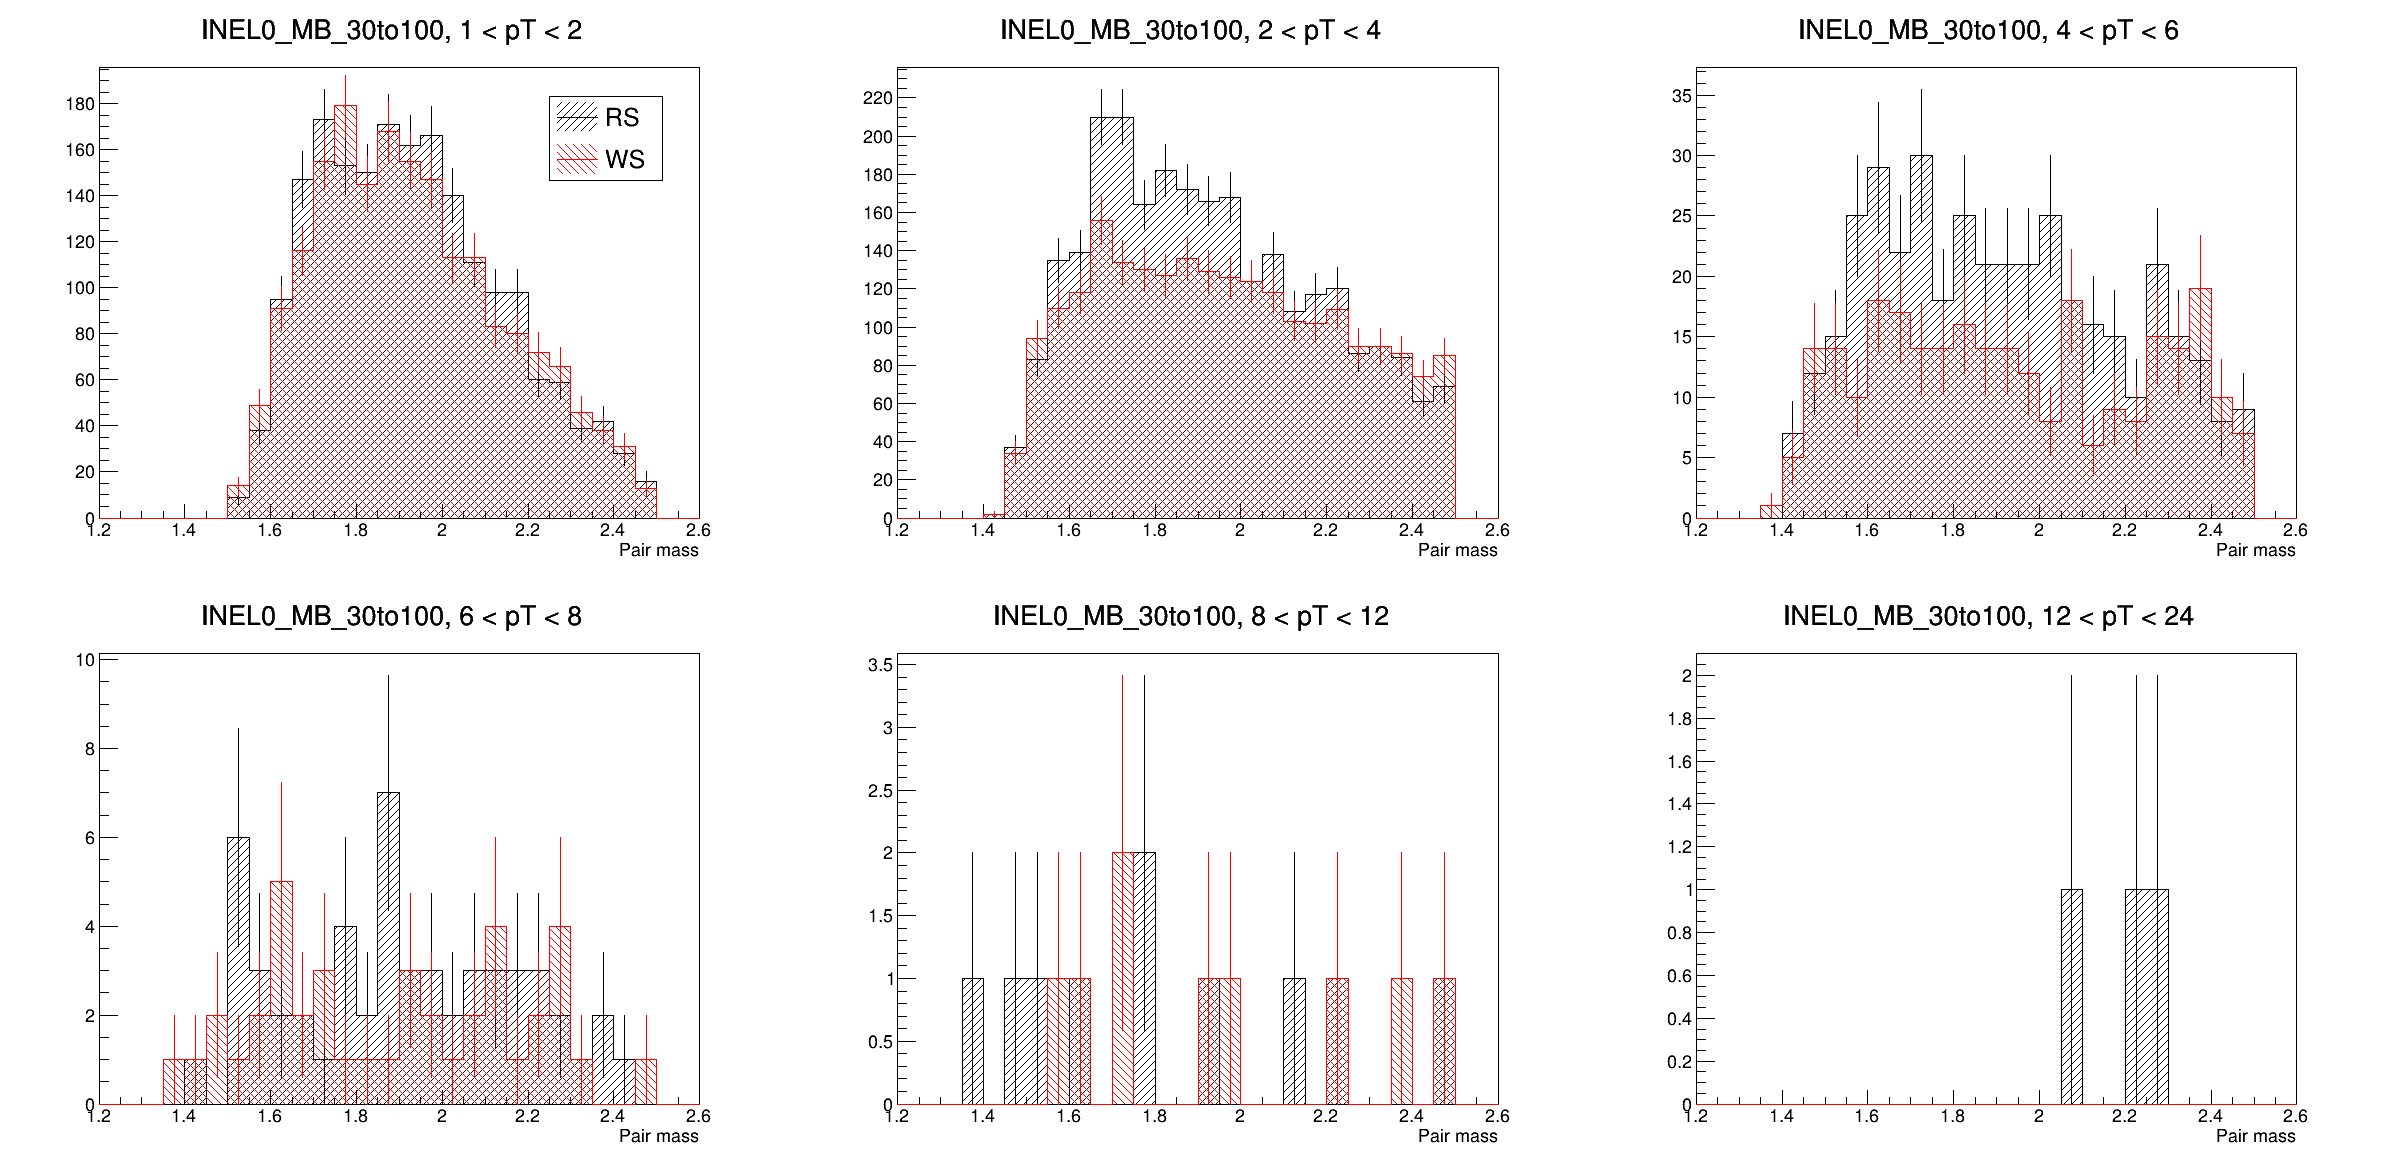
\includegraphics[width=0.75\textwidth]{plots/s2_RSmWS_INEL0_MB_30to100.png} \\\vspace{5pt}
    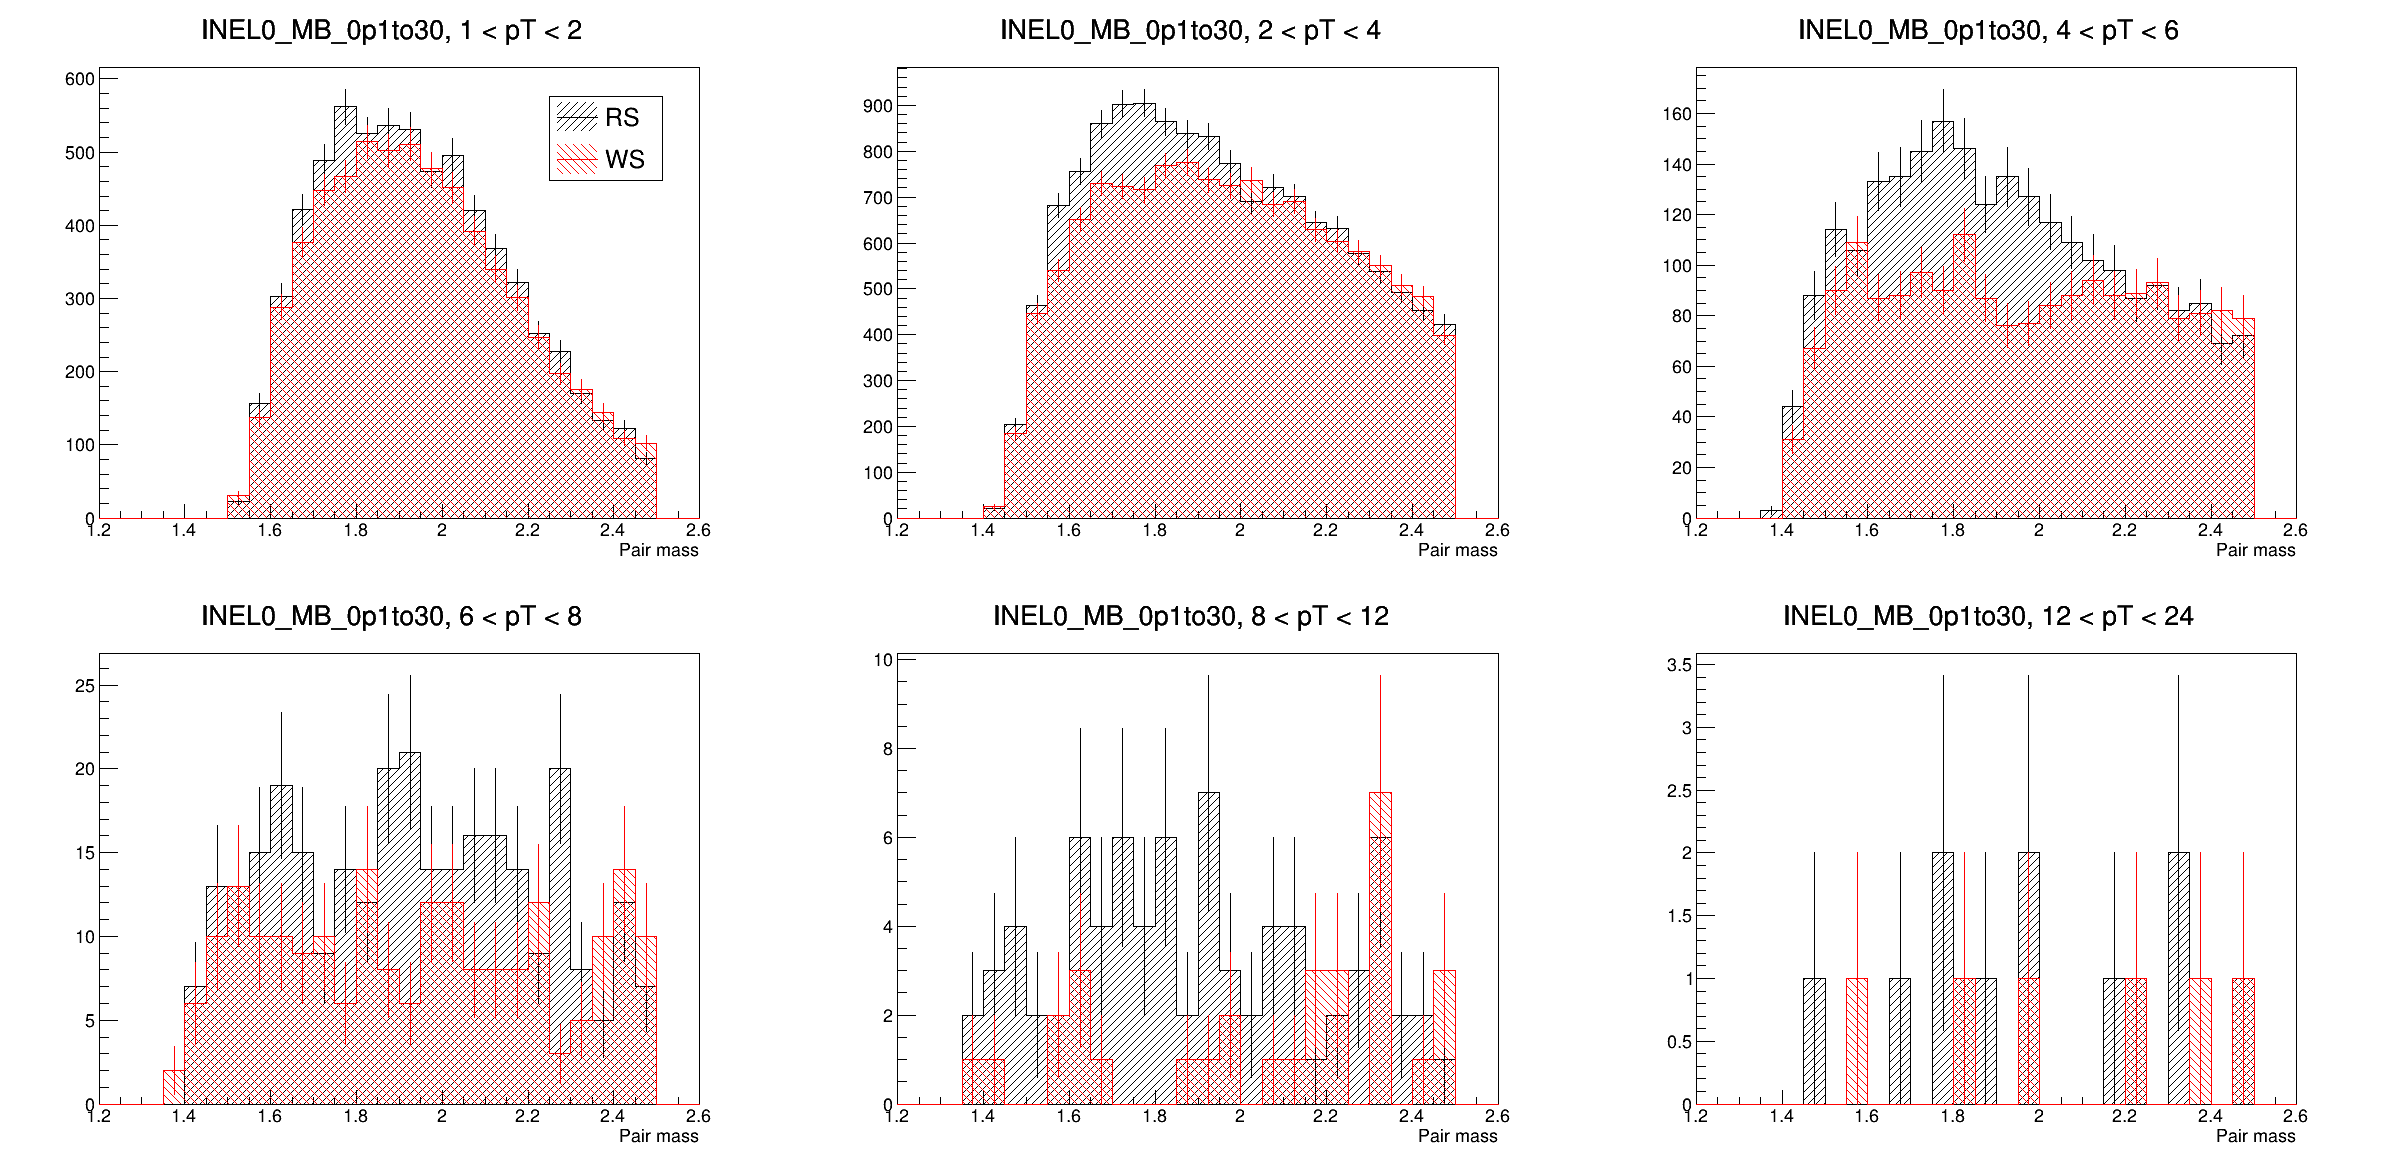
\includegraphics[width=0.75\textwidth]{plots/s2_RSmWS_INEL0_MB_0p1to30.png} \\\vspace{5pt}
    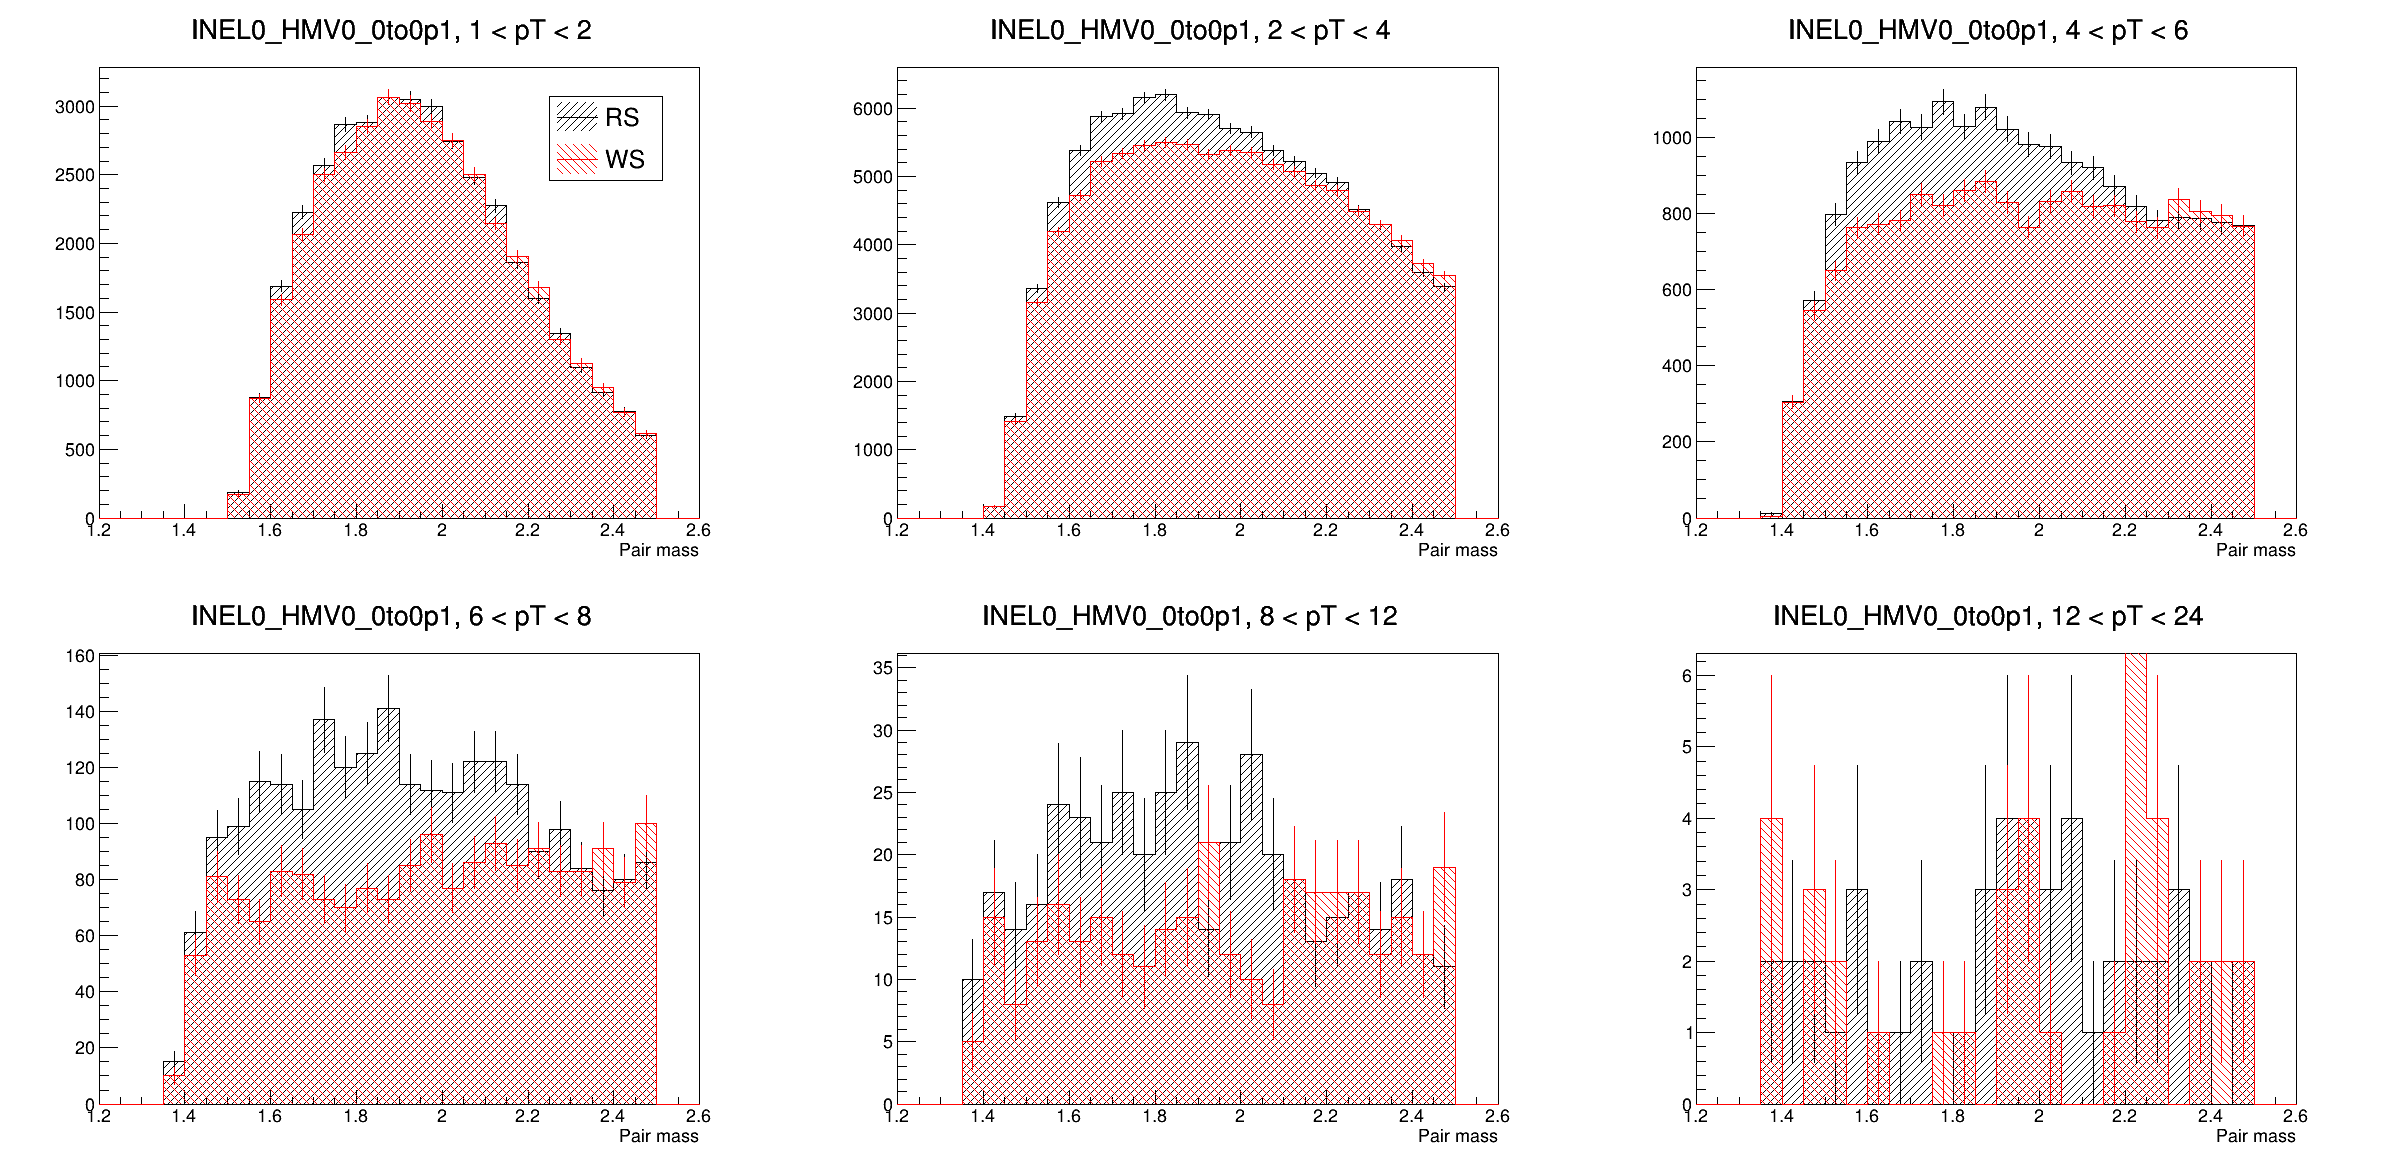
\includegraphics[width=0.75\textwidth]{plots/s2_RSmWS_INEL0_HMV0_0to0p1.png}
    \caption{\pt distributions of e\Xim pairs by sign (RS or WS), for configurations MB + [30, 100] (top 6),
    MB + [0.1, 30] (middle 6), and HMV0 + [0, 0.1] (bottom 6), respectively.}
    \label{fig:appB_RSWS}
\end{figure}
\clearpage

\begin{figure}[h]
    \centering
    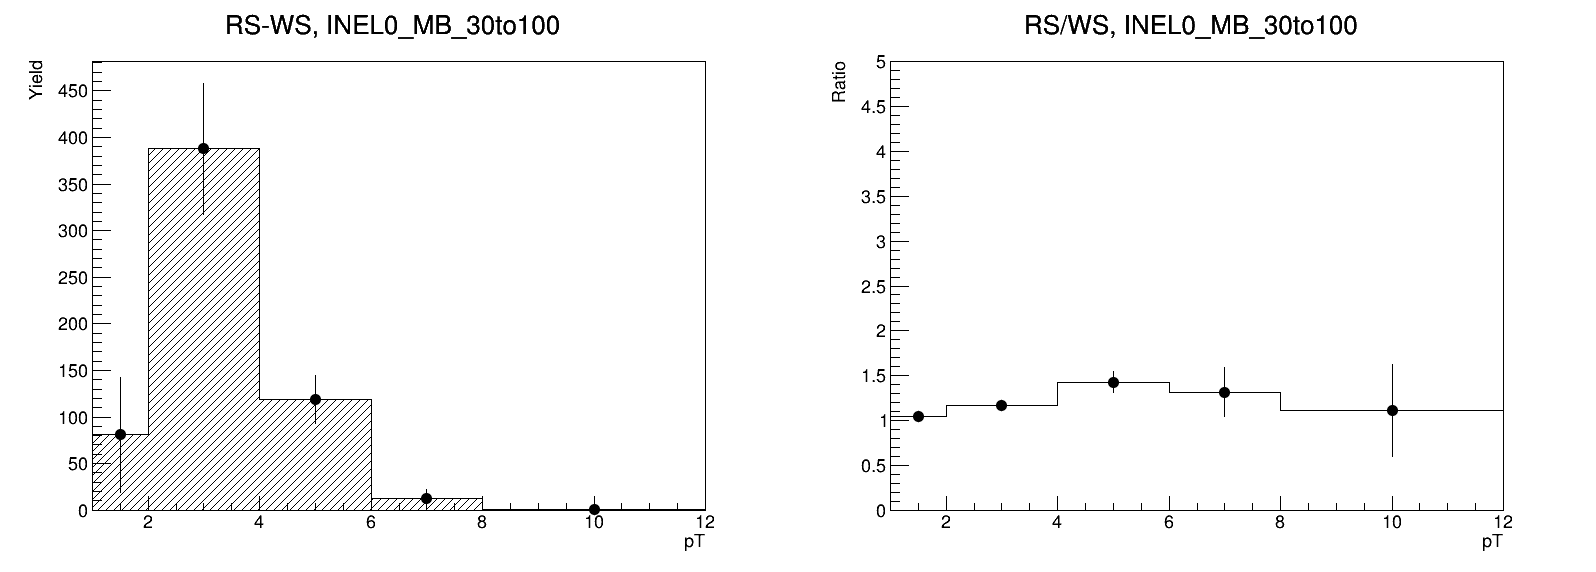
\includegraphics[width=0.95\textwidth]{plots/s2_RSdWS_INEL0_MB_30to100.png} \\\vspace{5pt}
    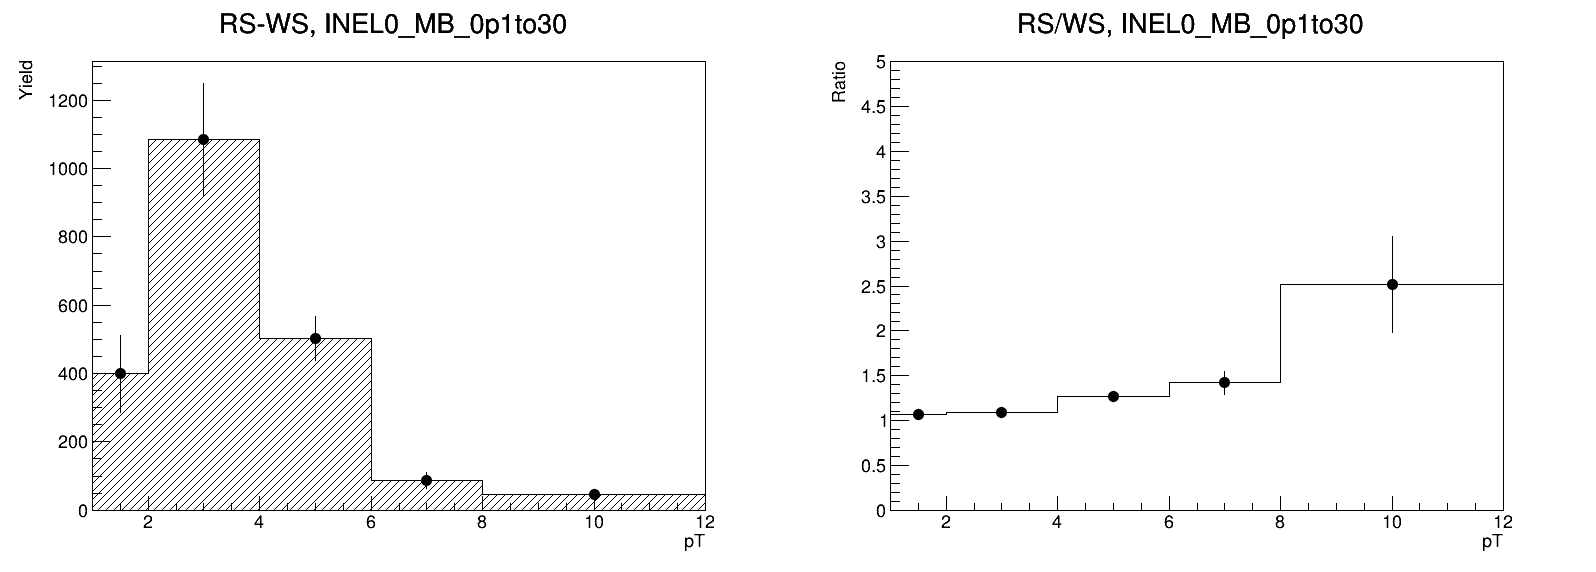
\includegraphics[width=0.95\textwidth]{plots/s2_RSdWS_INEL0_MB_0p1to30.png} \\\vspace{5pt}
    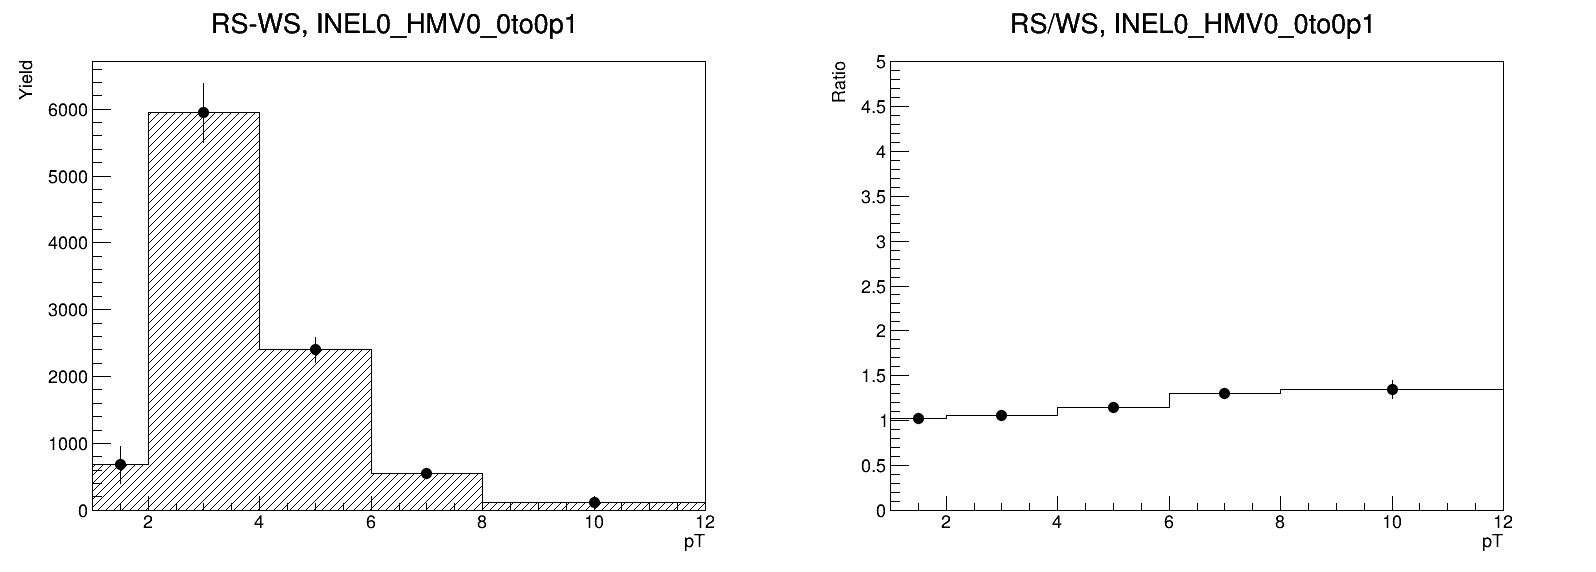
\includegraphics[width=0.95\textwidth]{plots/s2_RSdWS_INEL0_HMV0_0to0p1.png}
    \caption{\pt distributions of extracted signal by RS-WS (left) and ratio of RS/WS (right), for configurations MB + [30, 100] (top), MB + [0.1, 30] (middle), and HMV0 + [0, 0.1] (bottom), respectively.}
    \label{fig:appB_RSWSmd}
\end{figure}
\clearpage

\begin{figure}[h]
    \centering
    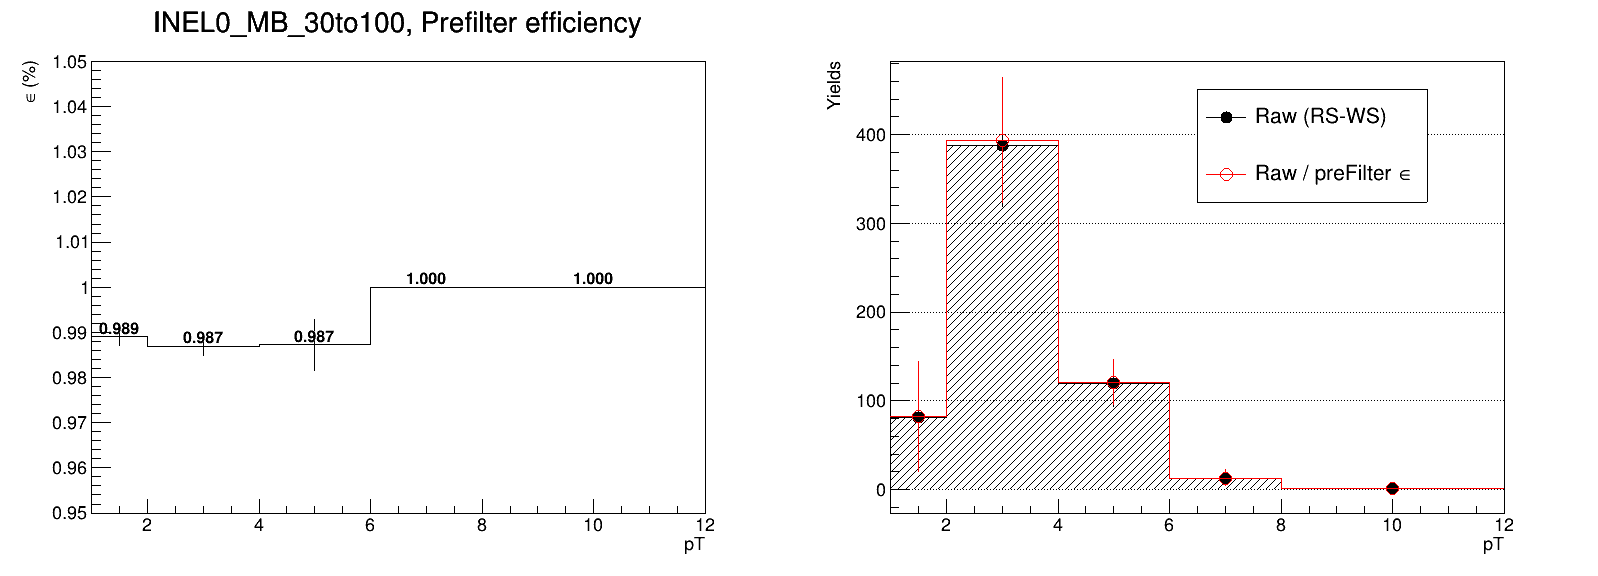
\includegraphics[width=0.95\textwidth]{plots/s2_preFCorr_INEL0_MB_30to100.png} \\\vspace{5pt}
    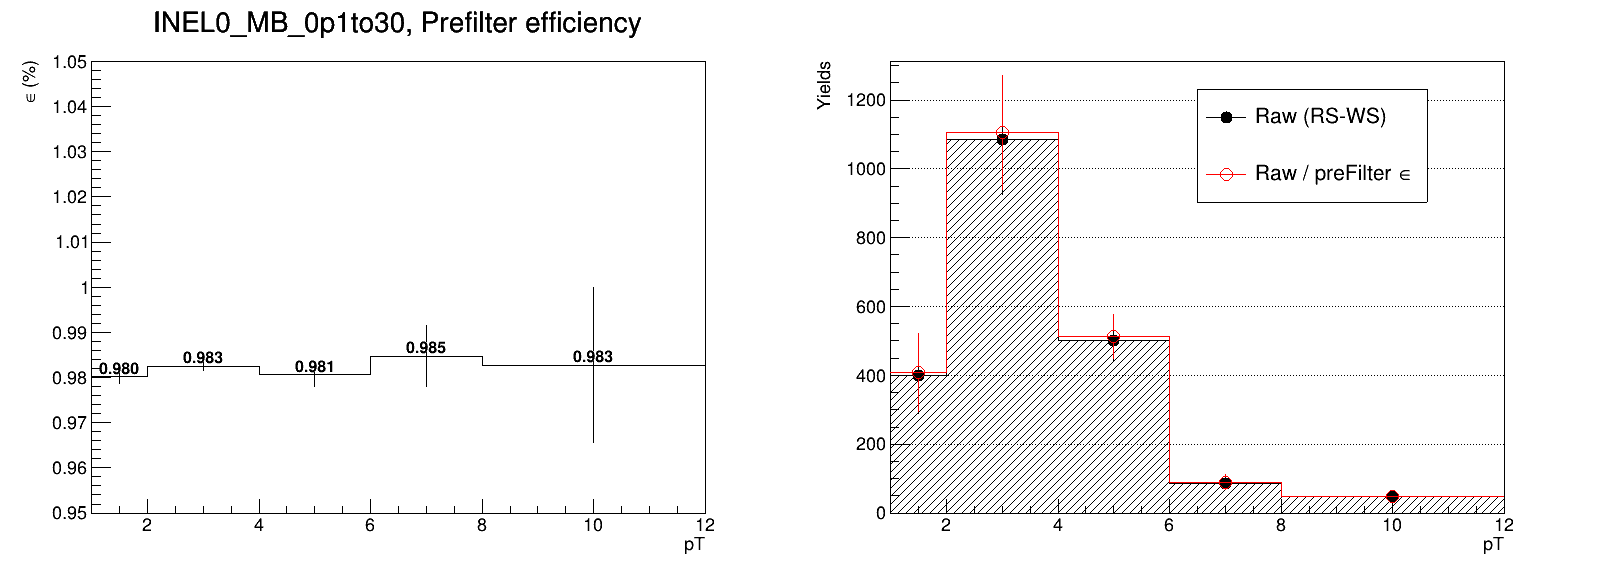
\includegraphics[width=0.95\textwidth]{plots/s2_preFCorr_INEL0_MB_0p1to30.png} \\\vspace{5pt}
    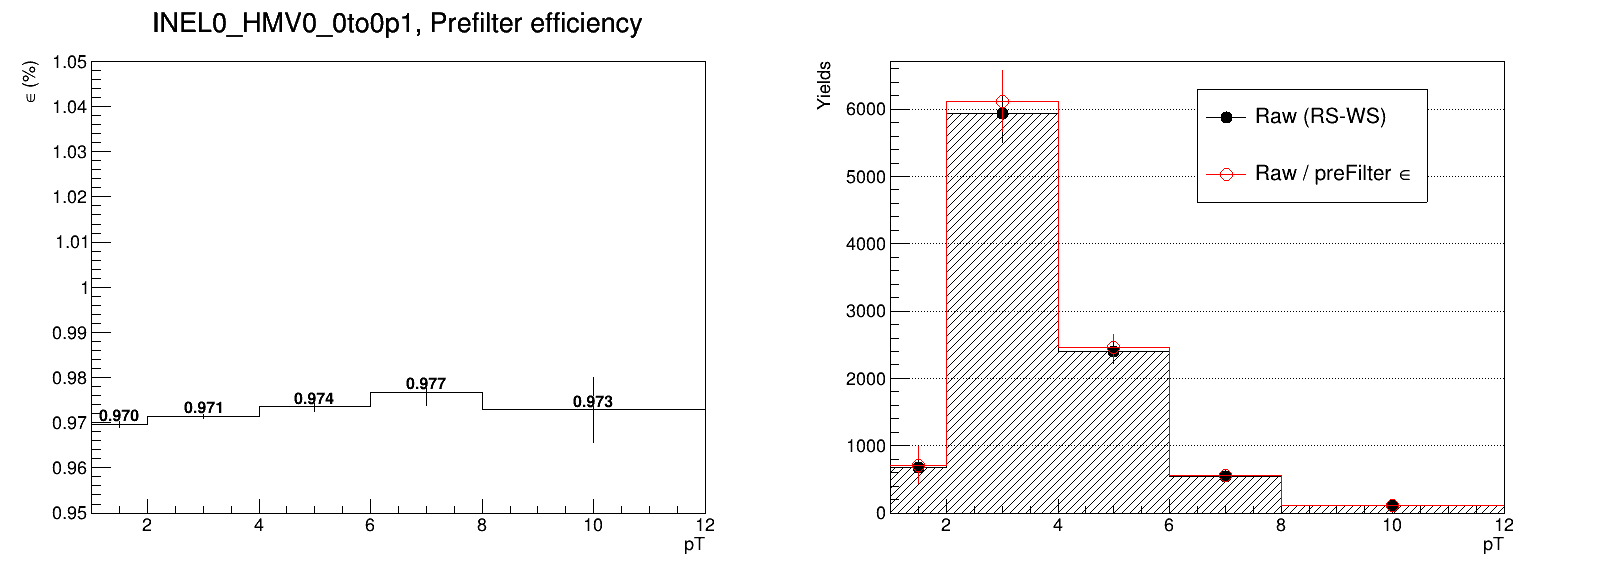
\includegraphics[width=0.95\textwidth]{plots/s2_preFCorr_INEL0_HMV0_0to0p1.png}
    \caption{Prefilter efficiency (left) and (RS-WS) yields before and after the correction (right), for configurations MB + [30, 100] (top), MB + [0.1, 30] (middle), and HMV0 + [0, 0.1] (bottom), respectively.}
    \label{fig:appB_preF}
\end{figure}
\clearpage

\begin{figure}[h]
    \centering
    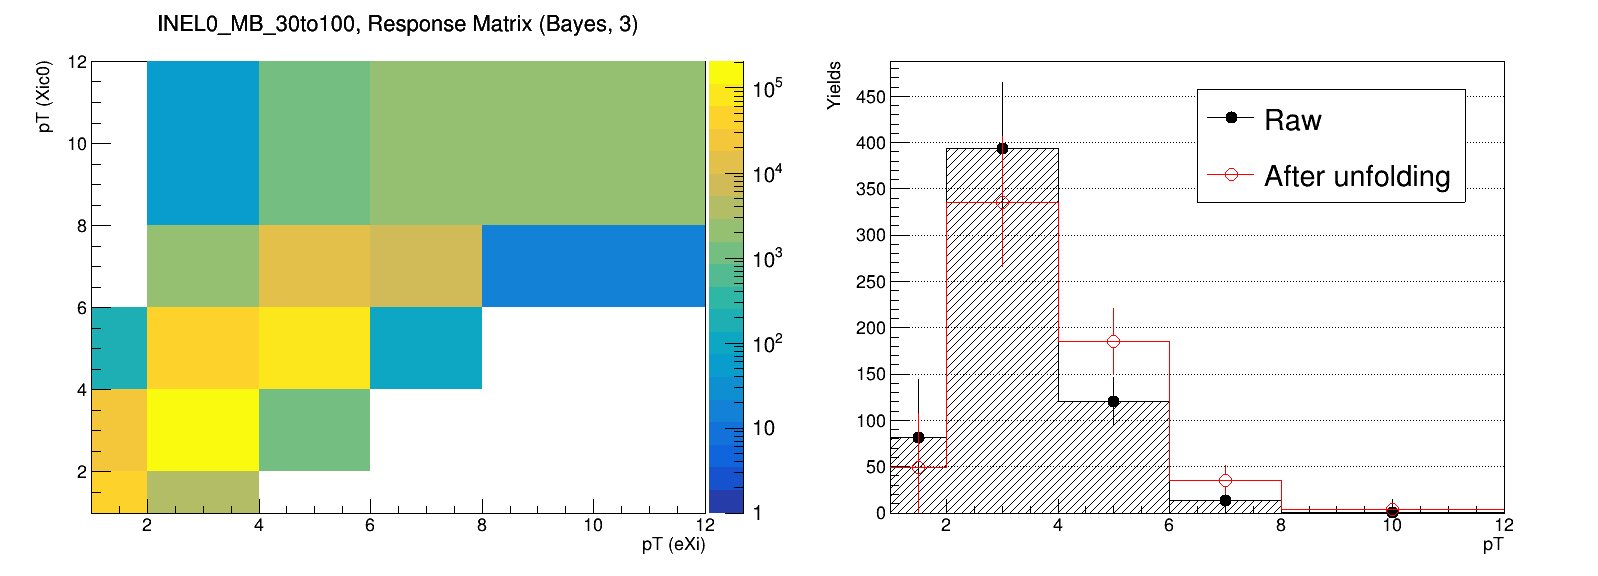
\includegraphics[width=0.95\textwidth]{plots/s2_unfold_INEL0_MB_30to100.png} \\\vspace{5pt}
    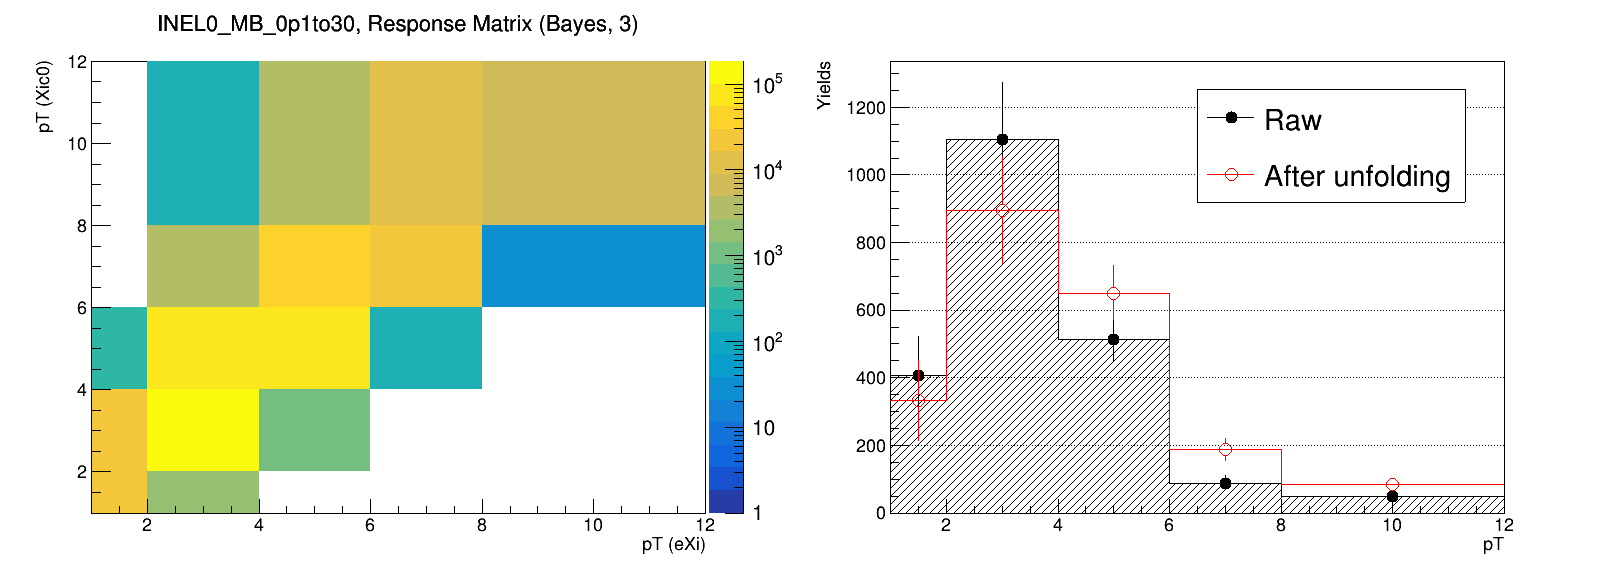
\includegraphics[width=0.95\textwidth]{plots/s2_unfold_INEL0_MB_0p1to30.png} \\\vspace{5pt}
    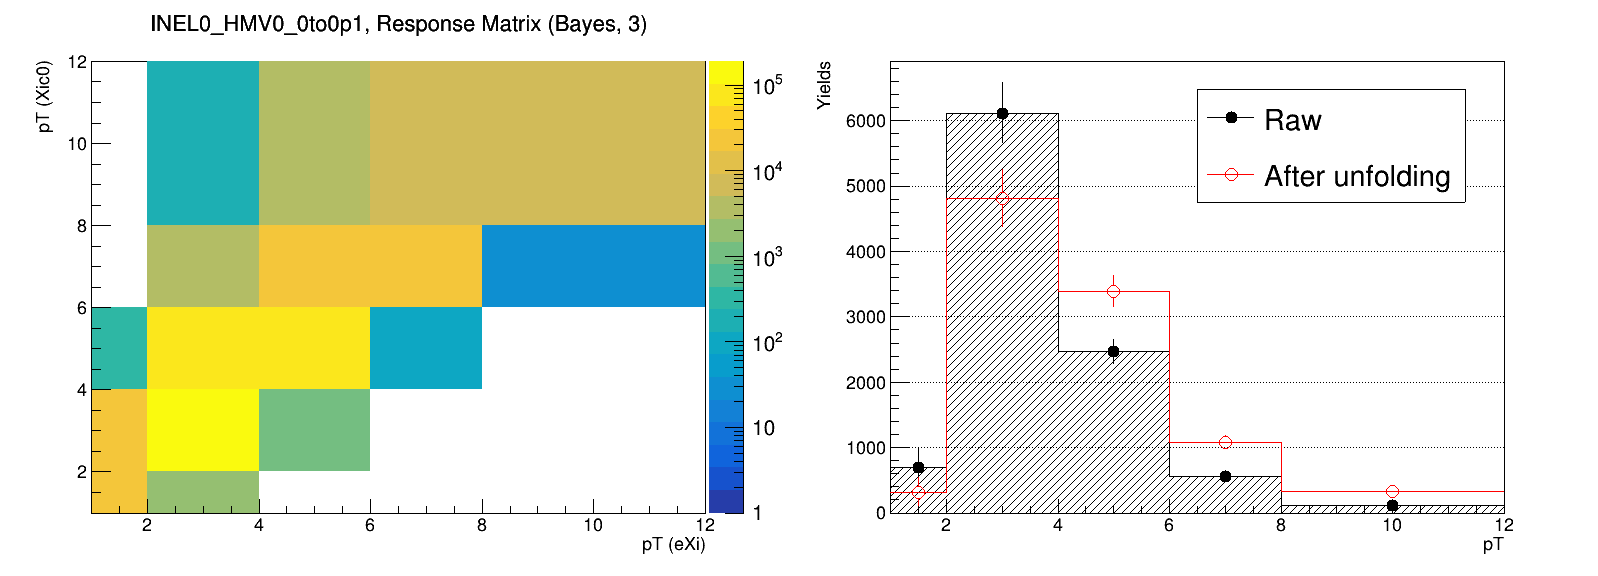
\includegraphics[width=0.95\textwidth]{plots/s2_unfold_INEL0_HMV0_0to0p1.png}
    \caption{\Xic - e\Xim response matrix by MC (left) and yields before and after the unfolding (right), for configurations MB + [30, 100] (top), MB + [0.1, 30] (middle), and HMV0 + [0, 0.1] (bottom), respectively.}
    \label{fig:appB_unfold}
\end{figure}
\clearpage

\begin{figure}[h]
    \centering
    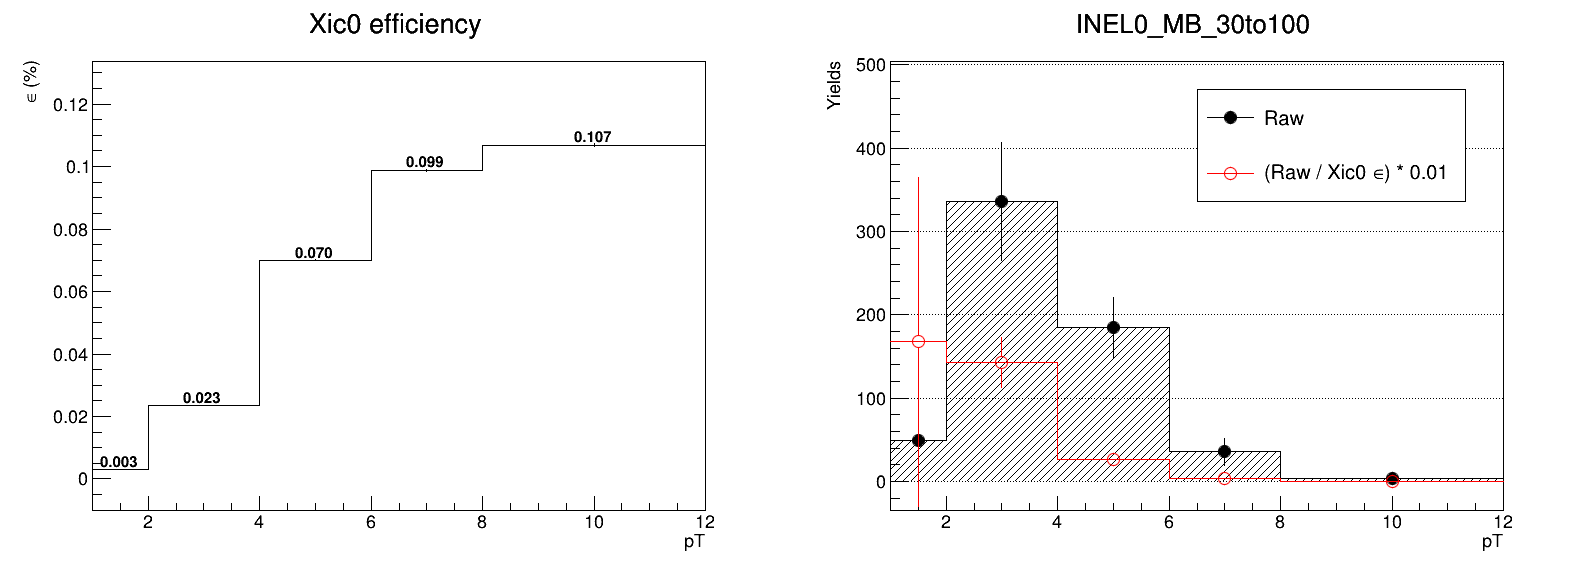
\includegraphics[width=0.95\textwidth]{plots/s2_Xic0Eff_INEL0_MB_30to100.png} \\\vspace{5pt}
    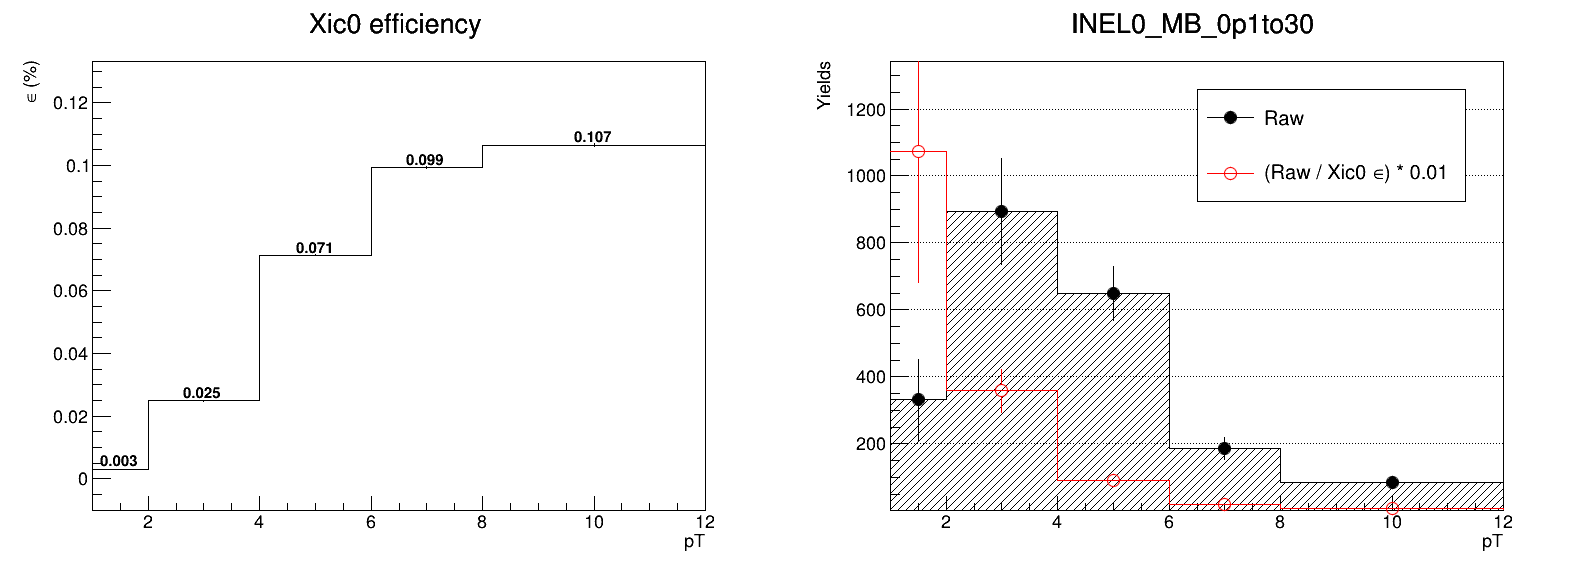
\includegraphics[width=0.95\textwidth]{plots/s2_Xic0Eff_INEL0_MB_0p1to30.png} \\\vspace{5pt}
    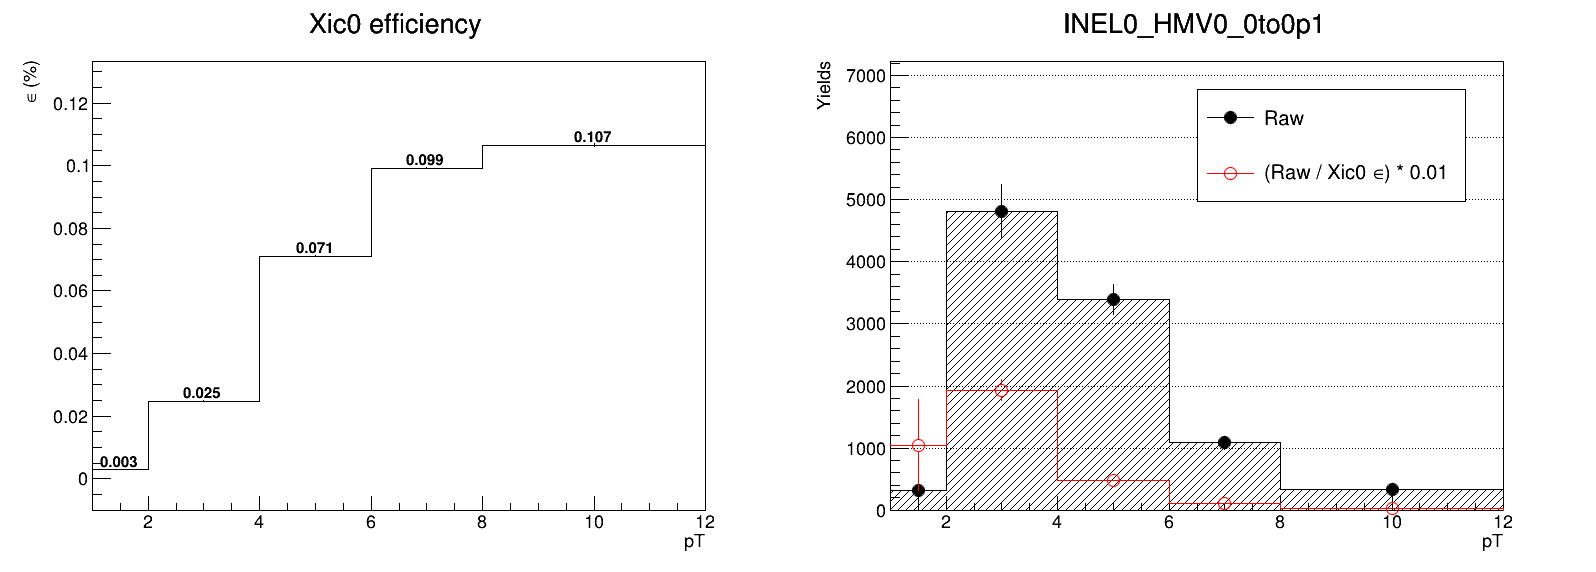
\includegraphics[width=0.95\textwidth]{plots/s2_Xic0Eff_INEL0_HMV0_0to0p1.png}
    \caption{$Acc \times \epsilon$ of \Xic (left) and Yields before and after correction (right)
    for configurations MB + [30, 100] (top), MB + [0.1, 30] (middle), and HMV0 + [0, 0.1] (bottom), respectively.}
    \label{fig:appB_eff}
\end{figure}
\clearpage

%--------------------------------------------
\end{appendix} \clearpage
%
\bibliographystyle{utphys}
\bibliography{secZ_bib}
\end{document}